% master.tex : master-fil for projektet
% ------------------------------------------------------------------------------
% Dette er hovedfilen for projektet, hvori indhold fra alle input-filer (tekst,
% billeder, litteraturdatabaser, osv.) samles

% Dokumenttypen 'book' er valgt pga. dens mange fleksible indstillinger
% Se https://tex.stackexchange.com/a/36989/118167
\documentclass[11pt,a4paper,twoside,openright,danish]{book}

% Variabler, som bruges til automatisk at indsætte titel, forfattere, osv. på
% forsiden og titelbladet.
\def \projecttitle       {Optimering}
\def \projectsubtitle    {Lineær programmering}
\def \projecttheme       {Simplex}
\def \projectdegree      {Matematik}  % eller Matematik-Økonomi/Teknologi
\def \projectperiod      {Forårssemesteret 2020}
\def \projectnumber      {P2}
\def \projectgroup       {B305}
\def \projectauthors     {
  Caroline Nørskov Budsted Weje\\
  Henriette Høiberg Bjørn\\
  Jesper Soelberg Jensen\\
  Jonas Winther\\
  Katharina Bramsing Bach\\
  Mie Frederiksen Larsen
  % ...
}
\def \projectsupervisors {
  Projektvejleder 1\\
  Projektvejleder 2
  % ...
}

% Preamblet indeholder alle de indstillinger og makroer, som skal indsættes for
% hovedindholdet, og i denne skabelon samles det i filen aaumath.sty, som
% definerer en pakke, der kan indlæses med \usepackage.
\usepackage{aaumath}
\setlength{\parindent}{0cm}

% Dokumentets indhold indsættes mellem \begin- og \end-makroerne for
% 'document'-blokken
\begin{document}

% Dokumentets 'front matter' tælles ikke med ifm. antal sider og nummereres med
% romerske tal. Herunder hører f.eks. forsiden, titelbladet, forordet og
% indholdsfortegnelsen.
\frontmatter
% incl/misc/frontpage.tex : rapportens forside
% ------------------------------------------------------------------------------


\backgroundsetup{
  scale = 1,
  angle=0,
  opacity=1,
  contents = {
    
\includegraphics[width=\paperwidth,height=\paperheight]{fig/img/aau/waves.pdf}
  }
}
\BgThispage
\pdfbookmark[0]{Forside}{forside}
\begin{titlepage}
  \centering
  \phantom{}
  \vspace{2cm}

  % AAU-segl
  \begin{minipage}[c]{0.2\paperwidth}
    \centering
    \makebox[0pt]{
      % fig/tikz/aau-badge.tex : AAU-logo til forsiden
% ------------------------------------------------------------------------------

\begin{tikzpicture}
  % Tegn hvid cirkel og tilføj det gennemsigtige, blå logo ovenpå
  \node[circle,color=white,fill=white,minimum size=1.175\textwidth] at (0,0) {};
  \node at (0,0) {
\includegraphics[width=\textwidth]{fig/img/aau/logo-circle.pdf}};
\end{tikzpicture}

    }
  \end{minipage}

  % Hovedindhold
  \vspace{4cm}
  {\fontfamily{bch}\selectfont
    \fboxsep0pt\colorbox{white}{
      \begin{minipage}{\textwidth}
        \centering
        \color{AAUblue1}

        \vspace{2em}
        {\Huge\bfseries\projecttitle}

        {\Large\bfseries\projectsubtitle}

        \bigskip
        \parbox{\textwidth}{\centering\large\projectauthors}

        \bigskip
        {\bfseries\large{\projectnumber}-Projekt, Gruppe \projectgroup, \projectdegree}
        \vspace{2em}
      \end{minipage}
    }
  }

\end{titlepage}

% incl/misc/titlepage.tex : rapportens titelblad
% ------------------------------------------------------------------------------
% Titelbladet genereres af makroen \aautitlepage, som er defineret i
% /incl/pre/ext/aautitlepage.sty


\pdfbookmark[0]{Titelblad}{titelblad}
\aautitlepage{
  \projectinfo{
    \projecttitle
  }{
    \projecttheme
  }{
    \projectperiod
  }{
    Gruppe \projectgroup
  }{
    \parbox[t]{\textwidth}{\projectauthors}
  }{
    \parbox[t]{\textwidth}{\projectsupervisors}
  }{
    \today
  }
}{
  \textbf{Institut for Matematiske Fag}\\
  Skjernvej 4A\\
  DK-9220 Aalborg Ø\\
  \href{http://math.aau.dk}{http://math.aau.dk}
}{
  % incl/misc/abstract.tex : projektets abstract
% ------------------------------------------------------------------------------
% Et abstract er et kort resume af rapporten, som vises på titelbladet

Linear programming is used to optimize linear programming problems. In this project, different methods for solving linear programming problems. One method explored is the geometric method, in which the level sets are used to find the solution to the problem. The other method is the simplex method. Here, the geometric property of the simplex method is explored and used to deduce the simplex method. The simplex method uses linear algebra to jump between basic solutions, to find the optimal one. This is implemented by the full tabular method, the lexiographic rule and the big M-method. The big M-method is used to solve organizational problems. The found methods are then used, to solve a case about a company wanting to optimize their expenses to salary. 
}

% incl/misc/contents.tex :
% ------------------------------------------------------------------------------

\pdfbookmark[0]{Indhold}{indhold}

% Indstillingerne i denne fil er grupperet, så de ikke påvirker andre dele
\begingroup

% Slå twoside fra midlertidigt for at undgår sideskift
\makeatletter
\@twosidefalse
\makeatother

% Placer indholdsfortegnelsen på sin egen side (bedst når den kun fylder en side)
\tableofcontents
\clearpage

% Placer oversigtslisterne på efterfølgende sider
\let\clearpage\relax
\listoffigures
\lstlistofpro
\lstlistofalg

\endgroup


% Dokumentets 'main matter' (hovedindhold) er der, hvor det meste indhold skal
% sættes ind. Sider og overskrifter er nummererede med arabiske tal.
\mainmatter

% Input-filer bør opdeles således, at hver fil svarer til et kapitel. Makroen
% \include indsætter et sideskift og indholdet fra den givne stil.

%\chapter{Reminders}

forkortelser for sætninger korrolarer osv.
\begin{table}[h]
\begin{tabular}{|l|l|}
stn & sætning \\
lma & Lemma \\
prop & proposition \\
defn & definition \\
kor & korrolar \\
eks & eksempel \\
alg & algoritme
\end{tabular}
\end{table}
\chapter{indledning}

\chapter{Lineær algebra}
Dette kapitel er skrevet med udgangspunkt i 

Lineær algebra bruges til at løse lineære ligningssystemer. 
En af de mest nyttige algoritmer, til at løse sådanne ligningssystemer, er Gaussisk elimination, som vil blive beskrevet senere i dette kapitel.

\section{Matricer}
Lineære ligningssystemer kan opskrives i matricer. 
En matrix er defineret i Definition \ref{def:matricer}.

\begin{defn} [Matrix]\label{def:matricer}
En matrix er en rektangulær tabel over skalarer. 
Størrelsen på en matrix er $m \times n$, hvor $m$ er antal rækker og $n$ er antal søjler. 
En matrix kaldes kvadratisk hvis $m=n$. 
Skalaren i den $i$'te række og $j$'te søjle kaldes $(i,j)$-indgangen.
\end{defn}

Herunder ses en matrix $\underset{m \times n}{A}$ og dens indgange, $a_{i,j}$. Den $i$'te række i A betenges $\vec{a}_i$, mens den $j$'te søjle angives $\vec{A}_j$.

\begin{align*}
\underset{m \times n}{A} = \begin{bmatrix}
	a_{1,1} & a_{1,2} & \dots & a_{1,j} & \dots & a_{1,n} \\
	a_{2,1} & \ddots  &       &         &       & \vdots \\
	\vdots  &         & \ddots &        &       & \vdots \\
	a_{i,1} &         &       & a_{i,j} &       & \vdots \\
	\vdots  &         &       &         & \ddots& \vdots \\
	a_{m,1} & \dots   & \dots & \dots   & \dots & a_{m,n} 
\end{bmatrix}
\end{align*}

Matricer kan bruges til at vise mange forskellige ting fra den virkelige verden, det kan være antal af varer solgt fra forskellige butikker, eller prisen på forskellige produkter. 

\begin{eks}
Herunder ses en $4 \times 3$-matrix, der viser antallet af solgte varer fra tre forskellige butikker. Hver række i matricen repræsenterer en bestemt vare, mens hver søjle repræsenterer en butik. Den første række viser altså hvor mange trøjer hver butik har solgt.
\begin{align*}
\begin{matrix}
	Trøjer \\
	Kjoler \\
	Bukser \\
	Jakker
\end{matrix}
\begin{bmatrix}
	24 & 35 & 43 \\
	10 & 47 & 24 \\
	33 & 25 & 32 \\
	28 & 51 & 37
\end{bmatrix}
\end{align*}
I denne matrice kan man se, at der i dens $(2,3)$-indgang står $24$, hvilket betyder, at den tredje butik har solgt $24$ kjoler. Der står i dens $(3,1)$-indgang $33$, hvilket betyder, at den første butik har solgt $33$ par bukser.
\end{eks}

\begin{defn}[Transponeret matrix]
Lad $A$ være en $m \times n$ matrix. Så er den transponerede matrix, $A^T$, en $n \times n$ matrix, hvor hver indgang i $A^T$, $(i,j)$ er den $(j,i)$'te indgang i $A$
\label{def:(transmatrix)} 
\end{defn}
Det vil sige at rækkerne i $A$, bliver til søjlerne i $A^T$. Og søjlerne i $A$ bliver til rækkerne i $A^T$.

\begin{eks}
Givet en matrix $A$ 	bestemmes nu den transponerede
\begin{align*}
A = \begin{bmatrix}
	5 & 3 & 3 \\
	1 & 2 & 5
\end{bmatrix}
\end{align*}

\begin{align*}
A^T = \begin{bmatrix}
	5 & 1  \\
	3 & 2  \\
	3 & 5
\end{bmatrix}
\end{align*}
Det ses at $A$ er en $2 \times 3$ matrix og $A^T$ er en $3 \times 2$ matrix. 
\end{eks}


En bestemt type af matrix er en identitetsmatrix, der betegnes $I_n$. 

\begin{defn} [Identitetsmatrix]\label{def:imatrix}
For hvert positivt heltal $n$, er $n \times n$ identitetsmatricen, $I_n$, den $n \times n$ matrix, hvor hver søjle er standardvektorerne $\vec{e_1}$, $\vec{e_2}$, $\dots$, $\vec{e_n}$ i $\mathbb{R}^n$.
\end{defn}

En identitetsmatrix med $3$ rækker og $3$ søjler, ser således ud:
\begin{align*}
I_3 = \begin{bmatrix}
	1 & 0 & 0 \\
	0 & 1 & 0 \\
	0 & 0 & 1 
\end{bmatrix}
\end{align*}

\begin{defn} [Delmatrix]\label{delmatrix}
En matrix $A'$ er en delmatrix af $A$, hvis $A'$ kan dannes ved at fjerne hele søjler og/eller hele rækker fra $A$.
\end{defn}

Givet en matrix $A$ kan der dannes delmatricen $A'$.

\begin{align*}
A = \begin{bmatrix}
	1 & 2 & 3 \\
	4 & 5 & 6 \\
	7 & 8 & 9 
\end{bmatrix}
\end{align*}

\begin{align*}
A' = \begin{bmatrix}
	5 & 6 \\
	8 & 9
\end{bmatrix}
\end{align*}

\section{Vektorer}
En vektor er en matrix, der enten kun har en søjle eller en række. Vektorer kan også repræsenteres geometrisk hvor en vektor er en pil med en retning og en længde.
Det vil sige, at en vektor er et særtilfælde af en matrix, og alle regneregler for matricer, gør sig derfor gældende for vektorer, men ikke alle regneregler for vektorer kan bruges for matricer.
En vektor med kun én søjle kaldes en søjlevektor, mens en vektor med kun én række kaldes en rækkevektor.
Vektorer anvendes blandt andet til at repræsentere rækker og søjler i matricer. 
I dette tilfælde er vektorerne derved delmatricer af den originale matrix.
Indgangene i en vektor kaldes vektorens vektorkomponenter, og svarer til vektorens koordinater i den geometriske repræsentation.

\begin{defn}[Søjlevektor]
Lad $A$ være en $m \times n$ matrix, så vil en \textbf{søjlevektor} være en delmatrix med kun en søjle, og med alle søjlens rækkekomponenter.
\begin{align*}
\vec{v}=\vec{A}_j = 
\begin{bmatrix}
a_{1,j}\\
a_{2,j}\\
\vdots \\
a_{m,j} \\
\end{bmatrix},\qquad  i\in \{1,...,n\}
\end{align*}
Vektoren $\vec{v}$ siges at have dimension $m$ og tilhører  $\mathds{R}^m$.
\end{defn}

På samme måde kan en rækkevektor defineres


\begin{defn}[Rækkevektor]
Lad $A$ være en $m \times n$ matrix, så vil en \textbf{rækkevektor} $\vec{v}$ være en delmatrix med kun en række og med alle rækkens søjlekomponenter.
\begin{align*}
\vec{v}=\vec{a}_i = 
\rvect{a_{i,1} & a_{i,2} & \dots & a_{i,n}},
\qquad  j\in \{1,...,m\}
\end{align*}
Vektoren $\vec{v}$ siges at have dimension $n$ og tilhører $\mathds{R}^n$.
\end{defn}
Bemærk at hvis henholdsvis $m$ eller $n$ er $1$, så er matricen i forvejen en vektor.\\

\subsection{Standard basis vektorer}
Standard basis vektorer er vektorer, hvis koordinater alle er $0$ pånær én, der har længden $1$ ud af aksen i det rum, $\mathds{R}^n$, vektoren er i. Standard basis vektorer i $\mathds{R}^n$ skrives som $\vec{e_i}$, hvor $i\in \{1,..,n\}$, hvor $i$ er den vektorkomponent, som har værdien $1$. 

\begin{defn}[Standard basis vektorer]
Lad $\vec{e}_{i}\in\mathds{R}^n$ være en vektor hvis $j$'te indgang er givet ved
\begin{align*}
\vec{e}_{i_{j}}=\begin{cases} 0, \quad j \neq i
\\ 1 , \quad j = i \end{cases}.
\end{align*}

\end{defn}



\section{Regneoperationer med matricer}
Givet to $m \times n$ matricer $A$ og $B$ kan der udføres forskellige regneoperationer. 
Summen af to matricer findes ved at addere en indgang i $A$ med tilsvarende indgang i $B$, så $A+B$ er en $m \times n$ matrix, hvor indgang $(i,j)$ er $a_{i,j}+b_{i,j}$. 
Det samme gør sig gældende ved substraktion. \\
Givet en $m \times n$ matrix $A$ og en skalar $c$, er produktet af skalaren og matricen, $cA$, en $m \times n$ matrix, hvor indgangene er $c$ gange den tilsvarende indgang i $A$. \\

\begin{stn}
Lad $A$, $B$ og $C$ være $m \times n$ matricer, og lad $s$ og $t$ være tilfældige skalarer. 
Så gælder følgende
\begin{enumerate}[label=(\alph*)]
\item $A + B = B + A$
\item $(A + B) + C = A + (B + C)$
\item $A + O = A$
\item $A + (-A) = O$
\item $(st) A = s (tA)$
\item $s(A + B) = sA + sB$
\item $(s+t)A = sA + tA$
\end{enumerate}
\label{stn_regn}
\end{stn}

\begin{proof} 
Lad $A$, $B$ og $C$ være $m \times n$ matricer. Lad matricen $O$ være en nulmatrix. \\
(a) Det vises, at enhver indgang i $A + B$ er tilsvarende i $B + A$. Betragt indgangene $a_{i,j}$ og $b_{i,j}$. Summen af $a_{i,j} + b_{i,j}$ er det samme som $b_{i,j} + a_{i,j}$. \\
(b) Det vises, at enhver indgang i $(A + B) + C$ er den samme som den tilsvarende indgang i $A + (B + C)$. Ligesom i (a) tages der udgangspunkt i indgang $(i,j)$. Summen af $(a_{i,j} + b_{i,j}) + c_{i,j}$ er det samme som $a_{i,j} + (b_{i,j} + c_{i,j})$. Ifølge den associative lov, er det uden betydning hvor paranteserne er placeret i et additionsudtryk. Derfor må indgangen $(i,j)$ i $(A + B) + C$ være lig indgang $(i,j)$ i $A + (B + C)$. \\
(c) For enhver indgang i $A$, $a_{i,j}$ skal denne adderes med $0$. Derfor må $A + O = A$. \\
(d) For enhver indgang i $A$, $a_{i,j}$ skal denne fratrækkes samme indgang i $A$, $a_{i,j}$. Derfor må $A + (-A) = O$. \\
(e) Her tages der udgangspunkt i den (i,j)-indgang af A, $a_{i,j}$. Det ses så, at udsagnet bliver til $(st)a_{i,j} = s(ta_{i,j})$ når flere tal multipliceres, er det lige meget i hvilken rækkefølge, dermed er (e) bevist. \\
(f) Hver indgang i A, $a_{i,j}$ lægges sammen med den tilsvarende indgang i B, $b_{i,j}$, dette giver venstresiden $s(a_{i,j}+b_{i,j})$. Da det er tilladt at multiplicere ind i en parantes, kan udtrykket skrives sådan, $s(a_{i,j}+b_{i,j})=sa_{i,j}+sb_{i,j}$, dermed er (f) bevist. \\
(g) På samme måde som før tages der udgangspunkt i den (i,j)-indgang af A, $a_{i,j}$. Udtrykket på venstresiden er så $(s+t)a_{i,j}$. Igen kan der multipliceres ind i parantesen og dermed fås følgende, $(s+t)a_{i,j}=sa_{i,j}+ta_{i,j}$, hvilket beviser (g).
\end{proof}

\begin{eks}
For at vise eksempler på nogle af de ovenstående regneoperationer, tages der udgangspunkt i matricerne A og B, samt skalaren s.
\begin{align*}
A= \begin{bmatrix}
	2 & 3 & 4 \\
	5 & -2 & 1 	
\end{bmatrix}  
B= \begin{bmatrix}
	1 & 2 & -1 \\
	-3 & 4 & 0
\end{bmatrix}  
s=2
\end{align*}
Først udføres regneoperation (a) fra Sætning \ref{stn_regn},
\begin{align*}
A+B= \begin{bmatrix}
	2 & 3 & 4 \\
	5 & -2 & 1 	
\end{bmatrix}  
+ \begin{bmatrix}
	1 & 2 & -1 \\
	-3 & 4 & 0
\end{bmatrix}
= \begin{bmatrix}
	3 & 5 & 3 \\
	2 & 2 & 1
\end{bmatrix}.
\end{align*}
Herfter udføres (f),
\begin{align*}
s(A+B)= 5 \times \left( \begin{bmatrix}
	2 & 3 & 4 \\
	5 & -2 & 1 	
\end{bmatrix}  
+ \begin{bmatrix}
	1 & 2 & -1 \\
	-3 & 4 & 0
\end{bmatrix} \right)
= 5 \times \begin{bmatrix}
	3 & 5 & 3 \\
	2 & 2 & 1
\end{bmatrix}
= \begin{bmatrix}
	15 & 25 & 15 \\
	10 & 10 & 5
\end{bmatrix}.
\end{align*}
\end{eks}


\subsection{Matrix produkt}
Multiplikation af to matricer gøres ikke ved af multiplicere på tilsvarende indegange i to matricer. Det at gange to matricer sammen defineres herunder. 
\begin{defn} [Matrix produkt]
Lad $A$ være en $m \times n$ matrix og $B$ være en $n \times p$ matrix. Da er en produktet $A \dot B$ en $m \times p$ matrix, hvor indgangene er givet ved: 

$$ad_{i,j} = \vec{a}_i \cdot \vec{B}_j$$

hvor $\vec{a}_i$ er den $i$'te række i $A$, og $\vec{B}_j$ er den $j$'te søjle i $B$
\label{def:(matrixprodukt)}
\end{defn}
Det er vigtigt at antallet af søjler i $A$ er det samme som antallet af rækker i $B$. Er det ikke tilfældet, så er matrix produktet ikke defineret. Matrix produktet er oftest ikke kommutativt. Ligningen $AB=AB$ er derfor ikke sjældent gældende. 
\begin{eks}
Nu tages udgangspunkt i to matricer $A$ og $B$. 
\begin{align*}
\underset{2 \times 3}{A}= \begin{bmatrix}
	\bf{1} & \bf{3} & \bf{-2} \\
	5 & 4 & 0 	
\end{bmatrix}  
\underset{3 \times 4}{B}= \begin{bmatrix}
	\bf{2} & 3 & -1 & 3 \\
	\bf{1} & 4 & 5 & 5\\
	\bf{1} & 0 & 4 & 2
\end{bmatrix}  
\end{align*}
For at beregne indgang $(1,1)$ benyttes række et i $A$ og søjle et i $B$. 
$$ab_{1,1}=1\cdot 2+3\cdot 1-2 \cdot 1 = 3$$ 
De resterende indgange beregens på samme måde. 
Matrix produkt af $A$ og $B$ er dermed givet ved:
\begin{align*}
\underset{2 \times 4}{AB}= \begin{bmatrix}
	\bf{3} & 15 & 6 & 14 \\
	14 & 31 & 15 & 35
\end{bmatrix}  
\end{align*}
\end{eks}

Hvis matrix produktet af to matricer, A og B, giver identitetsmatricen, sigen B matrix at være den inverse matrix til A. 
\begin{defn}[Invers matrix]
Lad $A$ og $B$ være kvadratiske $m \times m$ matricer. Lad $AB=BA=I_m$, hvor $I_m$ er identitetsmatricen. Så er A invertibel og B er den inverse matrix til A. 
\label{def(inversmatrix)}
\end{defn}

\begin{eks}
Givet en matrix A og en matrix B,
\begin{align*}
A= \begin{bmatrix}
1 & 3 \\
1 & 2
\end{bmatrix}
B= \begin{bmatrix}
-2 & 3 \\
1 & -1
\end{bmatrix}
\end{align*}
kan det undersøges om B er den inverse matrix til A, ved at finde matrix produktet AB.
\begin{align*}
\begin{bmatrix}
1 & 3 \\
1 & 2
\end{bmatrix}
\cdot \begin{bmatrix}
-2 & 3 \\
1 & -1
\end{bmatrix}
= \begin{bmatrix}
1 & 0 \\
0 & 1
\end{bmatrix}
\end{align*}
Fordi de to matricers produkt bliver identitetsmatricen $I_2$, kan det konkluderes, at B er den inverse matrix til A.
\end{eks}


\section{Lineære ligningssystemer}
Lineære ligninger, der indeholder ukendte variabler, kan skrives på formen

\begin{align*}
a_1x_1+a_2x_2+ \dots +a_nx_n = b,
\end{align*}

hvor $a_1, a_2, \dots , a_n$ og $b$ er reelle tal. 
Her kaldes $a_1,a_2, \dots , a_n$ koefficienter og $b$ er en konstant. En lineær ligning kunne for eksempel se sådan ud:

\begin{align*}
7x_1+3x_2-5x_3 = 10.
\end{align*}

Lineære ligninger må ikke indeholde to variable multipliceret, kvadratroden af en variabel, eller andet der gør den ikke-lineær. \\
Et sæt af $m$ lineære ligninger, der indeholder de samme $n$ variable, hvor både $n$ og $m$ er positive heltal, kaldes et lineært ligningssystem. Lineære ligningssystemer skrives på formen

\begin{align*}
a_{1,1}x_1+a_{1,2}x_2+ &\dots +a_{1,n}x_n = b_1\\
a_{2,1}x_1+a_{2,2}x_2+ &\dots +a_{2,n}x_n = b_2\\
&\vdots \\
a_{m,1}x_1+a_{m,2}x_2+ &\dots +a_{m,n}x_n = b_m
\end{align*}

Koefficienterne i et lineært ligningssystem kan skrives i en matrix, mens variable og konstanterne skrives som vektorer. Et lineært ligningsystem kan så skrives op som en matrix ligning på formen $A \vec{x} = \vec{b}$, hvor

\begin{align*}
A= \begin{bmatrix}
a_{1,1} & a_{1,2} & \dots & a_{1,n} \\
a_{2,1} & a_{2,2} & \dots & a_{2,n} \\
\vdots  &         &       & \vdots  \\
a_{m,1} & a_{m,2} & \dots & a_{m,n}
\end{bmatrix}, \ 
x= \begin{bmatrix}
x_1 \\
x_2 \\
\vdots \\
x_n
\end{bmatrix} og \ 
b= \begin{bmatrix}
b_1 \\
b_2 \\
\vdots \\
b_n
\end{bmatrix}
\end{align*}

Søjlerne i $A$ indeholder koefficienterne $x_1$, $x_2$, $\dots $, $x_n$ og kaldes derfor koefficientmatricen til det lineære ligningssystem. 
Den information, der er nødvendig for at løse et lineært ligningssystem, kan samles i en totalmatrix på formen:
\[
\left[
\begin{array}{cccc|c}
a_{1,1} & a_{1,2} & \dots & a_{1,n} & b_1 \\
a_{2,1} & a_{2,2} & \dots & a_{2,n} & b_2 \\
\vdots  &         &       &         & \vdots \\
a_{m,1} & a_{m,2} & \dots & a_{m,n} & b_n
\end{array}
\right]
\]

Totalmatricen laves ved at tilføje vektor $\vec{b}$ til koefficientmatricen $A$. Totalmatricen noteres således som $[A \ \vec{b}]$. \\

Løsningen til et lineært ligningssystem er en vektor i $\mathds{R}^n$, som ser således ud:

\begin{align*}
\begin{bmatrix}
s_1 \\
s_2 \\
\vdots \\
s_n
\end{bmatrix}
\end{align*}

Hvis $A$ er en $m \times n$ matrix, er en vektor $\vec{u}$  i $\mathds{R}^n$ en løsning til $A \vec{x}= \vec{b}$ hvis og kun hvis $A \vec{u}= \vec{b}$.

\begin{eks}
Følgende lineære ligningssystem er givet

\begin{align*}
8x_1+6x_2+4x_3 = 50 \\
2x_1+4x_2+6x_3 = 30.
\end{align*}

Dette kan så skrives i en matrix,

\begin{align*}
\begin{bmatrix}
8 & 6 & 4 & 50 \\
2 & 4 & 6 & 30
\end{bmatrix}.
\end{align*}

Løsningen til dette ligningssystem bliver følgende vektor

\begin{align*}
\begin{bmatrix}
2 \\
5 \\
1
\end{bmatrix}.
\end{align*}

Sætter man løsningen ind som variable fås følgende resultat,

\begin{align*}
8 \cdot 2 + 6 \cdot 5 + 4 \cdot 1 = 50 \\
2 \cdot 2 + 4 \cdot 5 + 6 \cdot 1 = 30.
\end{align*}

Det ses, at vektoren giver en rigtig løsning til ligningssystemet, fordi alle ligningerne går op når vektoren indsættes. 

\end{eks}


%\begingroup
%\tikzset{every picture/.style={scale=0.5}}%
\chapter{Lineær Programmering}
\textbf{Fokuspunkt: sammenskrivning af de to versioner}
Lineær programmering er en anvendelse af lineær algebra til at løse et optimeringsproblem. Lineære programmeringsproblemer tager udgangspunkt i maksimering eller minimering af en lineær funktion. For variablene er der fastsat en række af betingelser, som begrænser de mulige løsninger til problemet.
%Ved ikke: Må vi antage at læseren ved, hvad en lineær funktion er, for tror de ikke bare at det er ax +b?


Funktionen, som ønskes optimeret, kaldes \textbf{objektfunktionen}, og findes på formen:
\begin{align}
f(\vec{x})\ = \vec{c}^T \vec{x} \ =  c_1x_1 + c_2x_2 + \cdots + c_nx_n,
\end{align}
hvor $\vec{x}= \rvect{x_1 & x_2 & \cdots & x_n}^T$ og $\vec{c}= \rvect{c_1 & c_2 & \cdots & c_n}^T$.

\begin{comment}
Bør muligvis være en defintion, behøver ikke at skrives ud, men så skal f(\vec{x}) frem for f(x_1, ..., x_n).  Men det er jo variable repræcenteret ved en vektor så måske introducerer f(x_1, ..., x_n), udenfor definitionen.
\begin{defn}
Betragt et lineært programmerings problem, da er \textbf{objektfunktionen}
\begin{align*}
f(\vec{x}) = \vec{c}^T \cdot \vec{x}, 
\end{align*}
for $\vec{x}, \vec{c} \in \mathds{R}^n$, funktionen, som ønskes optimeret.
\end{defn} Eller noget, det er vigtigt at denne definition, vil kræve at vektor x og c bliver introduceret i den bindende tekst.
\end{comment}


%hvis objektfunktionen defineres, så bør det samme ske for bibetingelserne.
Dertil tilføjes en række af betingelser for variablene. Betingelser på formen
\begin{align}
	x_i \geq 0,
\end{align}
kaldes \textbf{positivitetsbetingelser}.
Andre lineære betingelser for variablene kaldes for \textbf{lineære bibetingelser}, og findes på formen, 
\begin{align}
	a_{i,1} x_1 + a_{i,2} x_2 + \cdots + a_{i,n} x_n \  = \ \vec{a}_i^T\vec{x} \ (\leq,=,\geq) \  b_i, \quad \text{for} \ i \in \{1,2,\cdots, m\}, %Kan man bruge \leq,=,\geq)?
\end{align}
hvor $m$ er antallet af lineære bibetingelser. I en lineær bibetingelse kan venstresiden være begrænset med $\leq, \geq$ eller $=$ i forhold til højresiden. I nogle typer af programmeringsproblemer anvendes kun en enkelt af disse relationer. Positivitetsbetingelser er et specialtilfælde af de lineære bibetingelser, da en positivitetsbetingelse, $x_i \geq 0$, blot kan ses som en lineær bibetingelse, hvor en koefficienten til $x_i$ er 1, mens resten af koefficienterne er 0 og hvor $b_i=0$.

En \textbf{mulig løsning} er en vektor $\vec{x}$, som overholder alle problemets betingelser. %Bør nok skrives som en definition, men det kan være at det først skal ske under geo? Bertimaz har i hvertfald en strangent def.

Et eksempel på et lineært programmeringsproblem ses i Eksempel \ref{eks:maksprob1}. Eksemplet er et lineært maksimeringsproblem, da objektfunktionen ønskes maksimeret.

\begin{eks}
Et eksempel på et lineært programmeringsproblem ses her, hvor funktionen $f(x_1,x_2)=4x_1+3 x_2$ skal maksimeres.
\begin{center}
\begin{tabular}{l	>{$}r<{$}	>{$}r<{$}	>{$}l<{$}}
Maksimer 		& 		4x_1&	+3 x_2	& \\
med hensyn til 	&  \ \ 	2 x_1& 	- 4 x_2	& \geq - 8\\
				&  		x_1& 	+3 x_2	& \leq 16\\
				&  \ \ 	x_1& 			& \leq 10\\
og $x_1,x_2\geq 0$
\end{tabular}
\end{center}


%Mængden af alle mulige løsninger til problemet kan vises grafisk. De mulige løsninger findes inden for det grå område på Figur \ref{fig:maksprob1}, hvor $x_1$ og $x_2$ vises henholdsvis på 1. og 2. aksen. %Hvor får du det grå område fra?
%
%\begin{center}
%	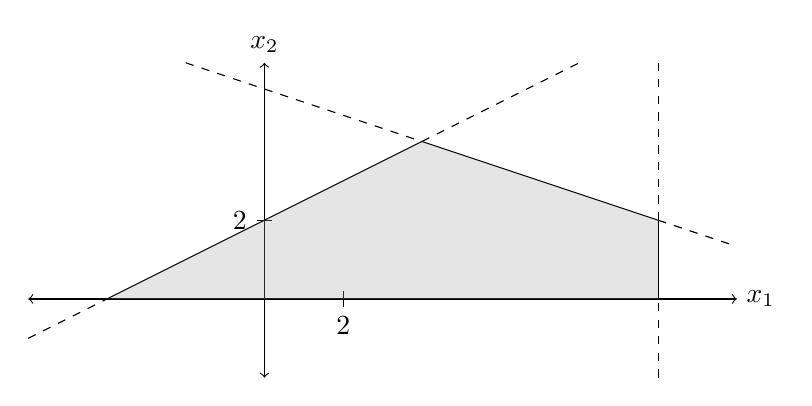
\begin{tikzpicture}
  %laver Grid
  	%\draw[thin,gray!40] (-3,-1) grid (6,3); 
  %x-aksen
  	\draw[<->] (-3,0)--(6,0) node[right]{$x_1$}; 
  %y-aksen
  	\draw[<->] (0,-1)--(0,3) node[above]{$x_2$};
  	
  %akse-markeringer
  	%\node[left] (xakse) at (0,1) {2};
  	\draw[] (-0.1,1) -- (0.1,1) node[pos=0,left] {2};
  	\draw[] (1,-0.1) -- (1,0.1) node[pos=0,below] {2};
  	
  %ligning 1
	\draw[domain=-3:-2,variable=\x,dashed] 	plot({\x},{0.5*\x+1});
	\draw[domain=-2:2,variable=\x] 			plot({\x},{0.5*\x+1});
	\draw[domain=2:4,variable=\x,dashed] 	plot({\x},{0.5*\x+1});
	
  %ligning 2
  	\draw[domain=-1:2,variable=\x,dashed] 	plot({\x},{-(1/3)*\x+8/3});
	\draw[domain=2:5,variable=\x] 			plot({\x},{-(1/3)*\x+8/3});
	\draw[domain=5:6,variable=\x,dashed] 	plot({\x},{-(1/3)*\x+8/3});
	

  %ligning 3
  	\draw[domain=-1:0,variable=\y,dashed] 	plot({5},{\y});
	\draw[domain=0:1,variable=\y] 			plot({5},{\y});
	\draw[domain=1:3,variable=\y,dashed] 	plot({5},{\y});

  %løsningsmængden skraveret
	\fill[gray!80,nearly transparent] (-2,0) -- (2,2) -- (5,1) --(5,0) --  cycle;
\end{tikzpicture}
%	\captionof{figure}{Grafisk repræsentation af mulige løsninger.}
%	\label{fig:maksprob1}
%\end{center} 

\label{eks:maksprob1}
\end{eks}

%%%%%%%%%%%%%%%%%%%%%%%%%%%%%%%%%%%%%%%%%%%%%%%%%%%%%%%%%%%%%%%%%%%%%%%%%%%%%%%%%%%%%%%%%%%%%%%%%%%%
%%%%%%%%%%%%%%%%%%%%%%%%%%%%%%%%%%%%%%%%%%%%%%%%%%%%%%%%%%%%%%%%%%%%%%%%%%%%%%%%%%%%%%%%%%%%%%%%%%%%%
Lineær programmering er en anvendelse af lineær algebra til at løse et optimeringsproblem. Lineære programmeringsproblemer tager udgangspunkt i maksimering eller minimering af en lineær funktion.
\begin{defn}[Lineær funktion]
Lad $f:\mathds{R} \to \mathds{R}$ være en funktion, da siges $f$ at være \textbf{lineær} hvis
\begin{enumerate}[label=\alph*]
\item $f(x_1 + x_2) = f(x_1) + f(x_2), \qquad \forall x_1,x_2 \in \mathds{R}$
\item $f(c\cdot x) = c \cdot f(x), \qquad \forall a, x \in \mathds{R}$
\end{enumerate}
\label{def:linfunk}
\end{defn}
Bemærk at selv om $f(x) = ax + b$ er kendt som en lineær funktion, er den ikke lineær pr Definition \ref{def:linfunk}.
Funktionen som skal optimeres kaldes objektfunktionen.
\begin{defn}
Betragt et lineært programmerings problem, da er \textbf{objektfunktionen}
\begin{align*}
f(\vec{x}) = \vec{c}^T \cdot \vec{x}, 
\end{align*}
for $\vec{x}, \vec{c} \in \mathds{R}^n$, funktionen, som ønskes optimeret.
\end{defn}
Objektfunktionen er repræsenteret som prikproduktet af en vektor $\vec{c}= \rvect{c_1 & c_2 & \cdots & c_n}^T$, der indeholder alle koefficienterne i funktionen og en vektor $\vec{x}= \rvect{x_1 & x_2 & \cdots & x_n}^T$, hvis indgange er funktionens variable.
Til objektfunktionen knyttes nogle bibetingelser, som variablene skal overholde. 
\begin{defn}[bibetingelser]
Lad $\vec{x}\in \mathds{R}$ repræsentere variabelene til et lineært programmeringsproblem, og $x_i$ for den $i$ indgang i $\vec{x}$ da kaldes betingelser på formen
\begin{enumerate}
\item \textbf{positivitetsbetingelser}: $x_i \geq 0$
\item \textbf{lighedsbetingelser}: $\vec{a}_i^T\vec{x} = b_i$
\item \textbf{størreendbetingelser}: $\vec{a}_i^T\vec{x} \geq b_i$
\item \textbf{mindreendbetingelser}: $\vec{a}_i^T\vec{x} \leq b_i$
\end{enumerate}
for $\vec{a_i}\in \mathds{R}^n$ og $b_i\in \mathds{R}$. 
Er $x_i$ ikke betinget af en positivitetsbetingelse kaldes den for en \textbf{frivariable}.
\end{defn}
Her betegner vektoren $\vec{a_i}$ koefficienterne i den $i$ bibetingelse, bemærk at hvis en ligning ikke indeholder den $j$ variable, da vil den $j$te indgang i koefficientvektoren $\vec{a_i}$ være lig nul, da der skal være en indgang pr variabel, ellers er prikproduktet ikke defineret. 

\section{Standard maksimerings- og minimeringsproblemer}
I et standard maksimeringsproblem gælder det, for alle bibetingelserne, at den lineære funktion af variablene er mindre end eller lig med en konstant.
Samtidig skal de i et standard minimeringsproblem være større end eller lig med en konstant. 
For begge problemer er variablene positivt begrænsede. 

Som beskrevet i Appendix \ref{afsnit:lign_sys} kan et lineært ligningssystem opskrives som et matrix-vektor produkt. 
Matricen repræsenterer koefficienterne i det lineære ligningssytem, mens variablene skrives som en vektor.
Tilsvarende gælder det for objektfunktionen, at denne kan skrives som et produkt af to vektorer. 
Dette tillader definitionen af et standard maksimeringsproblem med disse produkter i Definition \ref{def:std_maksmin}. 

\begin{defn}[Standard maksimering- og minimeringsproblemer]
	Lad $\vec{x}= \rvect{x_1 & x_2 & \cdots & x_n}^T$ være \textbf{løsningsvektoren} med koefficienter $\vec{c}= \rvect{c_1 & c_2 & \cdots & c_n}^T$ i objektfunktionen.
	Lad $A$ være en $m \times n$ matrix og lad $\vec{b}=\rvect{b_1 & b_2 & \cdots & b_m}^T$.\\
Da er standard maksimeringsproblemet defineret som
\begin{center}
\begin{tabular}{l	>{$}l<{$}}
Maksimer 		& \vec{c}^T\vec{x} \\
med hensyn til 	& A\vec{x} \leq \vec{b}\\
og 				& \vec{x} \geq \vec{0},
\end{tabular}
\end{center}
og standard minimeringsproblemet er defineret som
\begin{center}
\begin{tabular}{l	>{$}l<{$}}
Minimer			& \vec{c}^T\vec{x} \\
med hensyn til 	& A\vec{x} \geq \vec{b}\\
og 				& \vec{x} \geq \vec{0}.
\end{tabular}
\end{center}
\label{def:std_maksmin}
\end{defn}
Består ligningssystemet af ligheder, kaldes problemet henholdvist enten et \textbf{standard maksimeringsproblem med ligheder}, eller et \textbf{standard minimeringsproblem med ligheder}. \\

\begin{eks}[Standard maksimeringsproblem]
Hvis eksempel \ref{eks:maksprob1} skal omskrives til et standard maksimeringsproblem, skal alle  bibetingelserne være mindreendbetingelser.
Bibetingelse nr. 3 skal derved omskrives. Dette gøres ved at multiplicere begge sider af uligheden med $-1$, da dette vender ulighedstegnet. Derved bliver Eksempel \ref{eks:maksprob1} omskrevet til et standard maksimeringsproblem.
\begin{center}
\begin{tabular}{l	>{$}r<{$}	>{$}r<{$}	>{$}l<{$}}
Maksimer 		& 		4x_1	&	+3 x_2	& \\
med hensyn til 	&  \ \ 	-2 x_1	& 	+4 x_2	& \leq 8\\
				&  		x_1		& 	+3 x_2	& \leq 16\\
				&  \ \ 	x_1		& 			& \leq 10\\
og $x_1 \geq 0, x_2\geq 0$.
\end{tabular}
\end{center}
\label{eks:maksprob2}
\end{eks}

Bemærk, at på samme måde som bibetingelserne kan omskrives, kan et minimeringsproblem ligeledes laves til et maksimeringsproblem, ved at multiplicere med $-1$.



\begin{comment}
\begin{defn}[Standard minimum problem]
	Lad $\vec{x}= [x_1, x_2,\cdots, x_n]^T$ være \textbf{løsningsvektoren}, med koefficienter $\vec{c}= [c_1, c_2,\cdots, c_n]^T$ i objektfunktionen, og lad $m \times n$ matrixen $A=[A_{ij}]$ for $i=1,2,\cdots,m$ og $j=1,2,\cdots,n$ være begrænset af konstanterne $\vec{b}=[b_1, b_2,\cdots, b_m]^T$.
	Da er standard minimum problemet defineret som\\
\begin{center}
\begin{tabular}{l	>{$}l<{$}}
Minimer			& \vec{c}^T\vec{x} \\
med hensyn til 	& A\vec{x} \geq \vec{b}\\
og 				& \vec{x} \geq \vec{0}
\end{tabular}
\end{center}
\label{def:std_min}
\end{defn} %Hvorfor byttes der rundt på b og c? i min og max?


%%%%%%%%%%%%%%%%%%%%%%%%%%%%%%%%%%%%%%%%%%%%%%%%%%%%%%%%%%%%%%%%%%%%%%%%%%%%%%%%%%%%%%%%%%%%%%%%%%%%%%%%
%%%%%%%%%%%%%%%%%%%%%%%%%%%%%%%%%%%%%%%%%%%%%%%%%%%%%%%%%%%%%%%%%%%%%%%%%%%%%%%%%%%%%%%%%%%%%%%%%%%%%%%%%%

Det betyder at ethvert lineært programmeringsproblem kan omskrives, så det står på standardform.
\begin{defn}[Standard minimumsproblemer]
Lad $f(\vec{x}) = \vec{c}^T\vec{x}$ betegne objektfunktionen til et lineært minimeringsproblem, for $\vec{x},\vec{c} \in\mathds{R}^n$, lad $m \times n$ matricen $A=[A_{ij}]$ for $i=1,...,m$ og $j=1,...,n$, og lad $\vec{b} \in  \mathds{R}^n$.
Der er standard minimumsproblemet defineret som\\
\begin{center}
\begin{tabular}{l	>{$}l<{$}}
Minimer			& \vec{c}^T\vec{x} \\
med hensyn til 	& A\vec{x} \geq \vec{b}\\
og 				& \vec{x} \geq \vec{0}.
\end{tabular}
\end{center}
Består ligningssystemet af ligheder kaldes problemet; \textbf{standard minimumsproblem med ligheder}.
\label{def:std_maksmin}
\end{defn}
Bemærk at på samme måde som bibetingelserne kan omskrives, kan et minimeringsproblem laves til et maksimeringsproblem ved at multiplicere med $-1$, hvorfor at alle definitioner og sætninger er ækvivalente. Derfor defineres begreber og sætninger kun for minimums problemer, mens eksemplerne illustrere maksimums problemer.
\end{comment}
\subsection{Omskrivning mellem ligheder og uligheder}
Da et programmeringsproblem ikke nødvendigvis er på den ønskede form fra start af, er det vigtigt at kunne omskrive mellem uligheder og ligheder.\\
\begin{itemize}
\item Omskrivning mellem uligheder %Det er blevet bedere, men er stadig ikke helt godt
\begin{align*}
	\vec{a}_i^T\vec{x} \geq b_i \quad \Leftrightarrow \quad -\vec{a}_i^T\vec{x} \leq -b_i
\end{align*}
\item Omskrivning fra lighed til ulighed % hvorfor bruges der forskellige pile. rettet
\begin{center}
\begin{tabular}{>{$}l<{$} >{$}r<{$}}
	\vec{a}_i^T\vec{x} = b_i \quad \Leftrightarrow \quad 	& 
	\vec{a}_i^T\vec{x} \leq b_i \quad \text{og} \quad  \vec{a}_i^T\vec{x} \geq b_i \\ %Ved ikke om det vil give mening at have dem på samme linje og bruge \wedge i stedet for og.
\end{tabular}
\end{center}
\item Omskrivning fra ulighed til lighed\\
En ulighed kan omskrives til en lighed ved indførslen af en ikke-negativ \textbf{slack-variabel}, som udgør forskellen mellem $\vec{a}_i^T\vec{x}$ og $b_i$ i uligheden. 
Slack-variablen indgår kun i denne række af koefficientmatricen og får koefficient $1$ eller $-1$ afhængigt af uligheden i bibetingelsen.%, hvis uligheden  For maksimeringsproblemer får variabellen en koefficient på 1 i koefficientmatricen og -1 for minimeringsproblemer.
%Et standard maksimeringsproblem kan derved omskrives til ligheder ved at indføre en slackvariabel $x_{n+i}$ for hver bibetingelse. 
\begin{center}
\begin{tabular}{ >{$}l<{$} >{$}l<{$} >{$}l<{$}}
	\vec{a}_i^T \vec{x}  \leq b_i & \Rightarrow & \vec{a}_i^T \vec{x} \ + \ x_{n+i} \ = b_i\\
	\vec{a}_i^T \vec{x}  \geq b_i & \Rightarrow & \vec{a}_i^T \vec{x} \ -\ x_{n+i} \ = b_i
\end{tabular} %Du skriver at du gør det for max, men du gør det også for min.
\end{center} % Itemmize fungere okay, for de to første men dette afsnit bliver for langt til at det kan være et punkt, i min optik.

\begin{comment}
Derved bliver betingelserne for henholdsvis et maksimeringsproblem og et minimeringsproblem omskrevet til:
\begin{align*}
	A' &=\rvect{A & I_m}\\
	A' &=\rvect{A & -I_m}
\end{align*}

\end{comment}
%Nok en god idet at komme med et eksemple så \vec{a_i} \vec{x} + x_{n+i} = b_i indflettet, på lige fod med for omskrivning af mellem uligheder.
\end{itemize}



\begin{eks}[Standard maksimumsproblem]
Hvis eksempel \ref{eks:maksprob1} skal omskrives til et standard maksimumsproblem, skal alle relationer i bibetingelserne være $\leq$. %pas på med matematiske tegn i bindende tekst.
Bibetingelse nr. 3 skal derved omskrives. Dette kan gøres ved at multiplicere begge sider af uligheden med $-1$, da dette vender ulighedstegnet. Derved bliver Eksempel \ref{eks:maksprob1} omskrevet til et standard maksimumsproblem.\\
\begin{center}
\begin{tabular}{l	>{$}r<{$}	>{$}r<{$}	>{$}l<{$}}
Maksimer 		& 		4x_1	&	+3 x_2	& \\
med hensyn til 	&  \ \ 	-2 x_1	& 	+4 x_2	& \leq 8\\
				&  		x_1		& 	+3 x_2	& \leq 16\\
				&  \ \ 	x_1		& 			& \leq 10\\
og $x_1 \geq 0, x_2\geq 0$.
\end{tabular}
\end{center}
%Man må vel ikke bare sige at x_1 \geq 0, men man skal sige at x_1 = x_3 - x_4, hvor x_3, x_4 \geq 0.

%\begin{center}
%	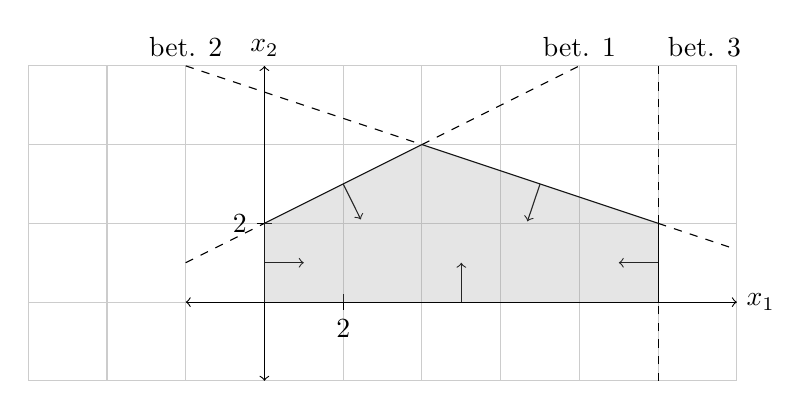
\begin{tikzpicture}
  %laver Grid. godt til når koordinater skal redigeres
  	\draw[thin,gray!40] (-3,-1) grid (6,3); 
  %x-aksen
  	\draw[<->] (-1,0)--(6,0) node[right]{$x_1$};
  	\draw[->] (2.5,0) -- (2.5,0.5);
  %y-aksen
  	\draw[<->] (0,-1)--(0,3) node[above]{$x_2$};
  	\draw[->] (0,0.5) -- (0.5,0.5);
  	
  %akse-markeringer
  	%\node[left] (xakse) at (0,1) {2};
  	\draw[] (-0.1,1) -- (0.1,1) node[pos=0,left] {2};
  	\draw[] (1,-0.1) -- (1,0.1) node[pos=0,below] {2};
  	
  %ligning 1
	\draw[domain=-1:0,variable=\x,dashed] 	plot({\x},{0.5*\x+1});
	\draw[domain=0:2,variable=\x] 			plot({\x},{0.5*\x+1});
	\draw[domain=2:4,variable=\x,dashed] 	plot({\x},{0.5*\x+1}) node[above] {bet. 1};
  	\draw[->] (1,1.5) -- (1.224,1.05);
	
  %ligning 2
  	\draw[domain=-1:2,variable=\x,dashed] 	plot({\x},{-(1/3)*\x+8/3}) node[above] at (-1,3) {bet. 2} ;
	\draw[domain=2:5,variable=\x] 			plot({\x},{-(1/3)*\x+8/3});
	\draw[domain=5:6,variable=\x,dashed] 	plot({\x},{-(1/3)*\x+8/3});
	\draw[->] (3.5,1.5) -- (3.34,1.026);

  %ligning 3
  	\draw[domain=-1:0,variable=\y,dashed] 	plot({5},{\y});
	\draw[domain=0:1,variable=\y] 			plot({5},{\y});
	\draw[domain=1:3,variable=\y,dashed] 	plot({5},{\y}) node[above right] {bet. 3};
	\draw[->] (5,0.5) -- (4.5,0.5);

  %løsningsmængden skraveret
	\fill[gray!80,nearly transparent] (0,0) -- (0,1) -- (2,2) -- (5,1) --(5,0) --  cycle;
\end{tikzpicture}
%	\captionof{figure}{Den mulige mængde af et standard maksimeringsproblem.}
%	\label{fig:maksprob2}
%\end{center}

\label{eks:maksprob2}
\end{eks}

%%%%%%%%%%%%%%%%%%%%%%%%%%%%%%%%%%%%%%%%%%%%%%%%%%%%%%%%%%%%%%%%%%%%%%%%%%%%%%%%%%%%%%%%%%%%%%
%%%%%%%%%%%%%%%%%%%%%%%%%%%%%%%%%%%%%%%%%%%%%%%%%%%%%%%%%%%%%%%%%%%%%%%%%%%%%%%%%%%%%%%%%%%%
Da bibetingelserne er ligninger repræsenteret ved et prikprodukt, kan hele ligningssystemet repræsenteres som et matrix-vektorprodukt, det kræver dog, at alle ikke positivitets betingelser er på samme form.
Det kan derfor være favorabelt at kunne omskrive fra en ulighed til en anden.
\begin{stn}
Lad $\vec{a}_i^T,\vec{x} \in \mathds{R}^n$ og $b_i \in \mathds{R}$, da gælder:
\begin{enumerate}
\item $\vec{a}_i^T\vec{x} \geq b_i \quad \Leftrightarrow \quad -\vec{a}_i^T\vec{x} \leq -b_i$
\item $\vec{a}_i^T\vec{x} = b_i \quad \Leftrightarrow  \quad  \vec{a}_i^T\vec{x} \leq b_i \quad \wedge \quad  \vec{a}_i^T\vec{x} \geq b_i$
\item $\vec{a}_i^T \vec{x}  \leq b_i \quad \Rightarrow \quad  \vec{a}_i^T \vec{x}  +  x_{n+i}  = b_i$
\item $\vec{a}_i^T \vec{x}  \geq b_i \quad \Rightarrow \quad  \vec{a}_i^T \vec{x}  - x_{n+i}  = b_i$
\end{enumerate}
hvor $x_{n+i}$ er en slack variable. 
\end{stn}
Dermed kan bibetingelserne skrives som $A\vec{x}\geq \vec{b}$, hvor $\vec{a_i}$ udgør den $i$te række i $A$ og $b_i$ er den $i$ indgang i $\vec{b}$.
Bemærk at positivitetsbetingelserne er et særtilfælde af størreendbetingelser, hvor en koefficienten til $x_i$ er 1, mens resten af koefficienterne er 0 og hvor $b_i=0$.
Positivitets betingelsen skrives ikke med i ligningssystemet, og i stedet er det som oftes underforstået, at enhver variable skal være ikke negativ.
For at det skal gøre sig gældende, skal en hver frivariable omskrives så de er betinget af en positivitetsbetingelse.
\begin{stn}
Lad $x_i$ være en frivariabel, da er $x_i = x_{n+i}-x_{n+i+1}$, hvor $x_{n+i},x_{n+i+1}\geq 0$.
\end{stn}
\section{Løsninger til linære programmeringsproblemer}

Den mulige mængde er mængden af løsningsvektorer, $\vec{x}$, som opfylder alle problemets betingelser. Hvis en optimal løsning eksisterer, vil denne derved være indeholdt i den mulige mængde.

\begin{defn}[Mulige løsninger og den mulige mængde]
En \textbf{mulig løsning} er en løsningsvektor $\vec{x}$, som opfylder alle problemets betingelser.\\
\textbf{Den mulige mængde} $\mathcal{F}$ er mængden af alle de mulige løsninger. Den vil derfor, for et standard maksimeringsproblem, være defineret som
\begin{align*}
\mathcal{F}=\{\vec{x} \in \mathds{R}^n|A\vec{x} \leq \vec{b}, \vec{x} \geq \vec{0}\}.
\end{align*}
Et problem kaldes \textbf{inkonsistent}  hvis den mulige mængde er den tomme mængde, ellers er problemet \textbf{konsistent}. 
\end{defn}

I lineær programmering søges der efter en optimal løsning, som vil være den mulige løsning, der enten maksimerer eller minimerer objektfunktionen, afhængig af, om der er tale om et maksimerings- eller minimeringsproblem. 
Husk på, at et maksimeringsproblem kan laves til et minimeringsproblem, hvorfor det kun er nødvendigt at definere den optimale løsningsværdi for minimeringsproblemet.
\begin{defn}[Optimal løsningsværdi]
Lad $f$ være objektfunktionen til et lineært minimeringsproblem, da kaldes en vektor $\vec{x}^*$ en \textbf{optimal løsningsværdi}, hvis 
\begin{align}
	f(\vec{x}^*)=\min\limits_{\vec{x} \in \mathcal{F}}f(\vec{x}).
\end{align}
Værdien af $f(\vec{x}^*)$ kaldes den \textbf{optimale værdi}.
\end{defn}

Den optimale løsning kan findes på forskellige måder, heriblandt med Simplex metoden, som beskrives i Kapitel \ref{chap:simp}. En anden måde er ved geometrisk visualisering af den mulige mængde. Denne metode er mulig for problemer med op til 3 variable, da løsningsmængden derved visualiseres som et plot i det tilsvarende antal dimensioner. De mulige løsninger findes således inden for det område, der er begrænset af betingelserne. 

\begin{eks}[Den mulige mængde]
Ved at indtegne betingelserne i et koordinatsystem er det muligt at visualisere den mulige mængde som fællesmængden af de mængder, der dannes ud fra betingelserne. På Figur \ref{fig:maksprob2} er den mulige mængde for problemet i Eksempel \ref{eks:maksprob2} indtegnet. Der er desuden tegnet en pil for hver betingelse, som viser, for hvilken side af linjen, koordinaterne opfylder betingelsen. Den mulige mængde er farvet grå.

\begin{center}
	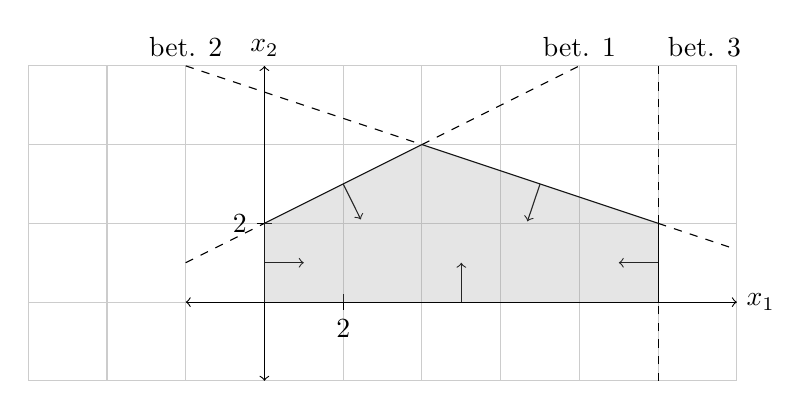
\begin{tikzpicture}
  %laver Grid. godt til når koordinater skal redigeres
  	\draw[thin,gray!40] (-3,-1) grid (6,3); 
  %x-aksen
  	\draw[<->] (-1,0)--(6,0) node[right]{$x_1$};
  	\draw[->] (2.5,0) -- (2.5,0.5);
  %y-aksen
  	\draw[<->] (0,-1)--(0,3) node[above]{$x_2$};
  	\draw[->] (0,0.5) -- (0.5,0.5);
  	
  %akse-markeringer
  	%\node[left] (xakse) at (0,1) {2};
  	\draw[] (-0.1,1) -- (0.1,1) node[pos=0,left] {2};
  	\draw[] (1,-0.1) -- (1,0.1) node[pos=0,below] {2};
  	
  %ligning 1
	\draw[domain=-1:0,variable=\x,dashed] 	plot({\x},{0.5*\x+1});
	\draw[domain=0:2,variable=\x] 			plot({\x},{0.5*\x+1});
	\draw[domain=2:4,variable=\x,dashed] 	plot({\x},{0.5*\x+1}) node[above] {bet. 1};
  	\draw[->] (1,1.5) -- (1.224,1.05);
	
  %ligning 2
  	\draw[domain=-1:2,variable=\x,dashed] 	plot({\x},{-(1/3)*\x+8/3}) node[above] at (-1,3) {bet. 2} ;
	\draw[domain=2:5,variable=\x] 			plot({\x},{-(1/3)*\x+8/3});
	\draw[domain=5:6,variable=\x,dashed] 	plot({\x},{-(1/3)*\x+8/3});
	\draw[->] (3.5,1.5) -- (3.34,1.026);

  %ligning 3
  	\draw[domain=-1:0,variable=\y,dashed] 	plot({5},{\y});
	\draw[domain=0:1,variable=\y] 			plot({5},{\y});
	\draw[domain=1:3,variable=\y,dashed] 	plot({5},{\y}) node[above right] {bet. 3};
	\draw[->] (5,0.5) -- (4.5,0.5);

  %løsningsmængden skraveret
	\fill[gray!80,nearly transparent] (0,0) -- (0,1) -- (2,2) -- (5,1) --(5,0) --  cycle;
\end{tikzpicture}
	\captionof{figure}{Skravering af den mulige mængde for et standard maksimeringsproblem.}
	\label{fig:maksprob2}
\end{center}
\end{eks}

Løsningerne til et optimeringsproblem er beskrevet som værende alle de vektorer, $\vec{x}$, som overholder bibetingelserne. Løsningsmængden til bibetingelserne er beskrevet som et polyeder.
\begin{defn} [Polyeder]
Et \textbf{Polyeder} er en mængde 
\begin{align*}
 P =\{ \vec{x} \in \mathds{R}^n | A \vec{x} \geq \vec{b}, \vec{b}\in \mathds{R}^m\},
\end{align*}
hvor $A$ er en $m \times n$ matrix.
\end{defn}
Hvis et lineært programmeringsproblem står på standardform med ligheder $\{ \vec{x} \in \mathds{R}^n | A \vec{x} = \vec{b}, \vec{b}\in \mathds{R}^m\}$, så kaldes det stadig et polyeder.\\
Hvis der er et polyeder $P=\{\vec{x} \in \mathds{R}\mid A\vec{x}=\vec{b},\vec{x}\geq \vec{0}\}$, som består af alle bibetingelserne for problemet, så må der også findes et andet polyeder $Q$, som består af alle de lineært uafhængige bibetingelser for problemet. Da $P$ består af de samme bibetingelser som $Q$ og lidt flere til, så er en løsning $\vec{x}$ til $P$ nødvendigvis også en løsning til $Q$, og modsat er en løsning til $Q$ også en løsning til $P$. Derfor må $Q=P$, hvilket vil blive vist i følgende sætning.

\begin{stn}[Q=P]
Lad $P=\{\vec{x} \in \mathds{R}^n\mid A\vec{x}=\vec{b},\vec{x}\geq \vec{0}\}$ være et ikke-tomt polyeder, hvor $A$ er en $m\times n$ matrix.\\
Antag at $rang(A)=k<m$ og at rækkerne $\vec{a_i}^T$ for $i=1,\dots ,k$ er lineært uafhængig. Betragt polyederet $Q=\{\vec{x} \in \mathds{R}^n\mid \vec{a_i}^T\vec{x}=b_{i}, \vec{x}\geq \vec{0}, i = 1,\dots	k\}$. Så er $Q=P$.
\label{stn:PQ}
\end{stn}

\begin{proof}
Hvis $P=\{\vec{x} \in \mathds{R}^n\mid A\vec{x}=\vec{b}, \vec{x}\geq \vec{0}\}$ er et polyeder med $rang(A)=k$, afgrænset af alle bibetingelserne, så må der være et polyeder $Q=\{\vec{x} \in \mathds{R}^n\mid \vec{a_i}^T\vec{x}=b_{i}, \vec{x}\geq \vec{0}, i = 1,\dots,	k\}$, der består af alle lineært uafhængige bibetingelser. Så må $P\subseteq Q$, eftersom alle elementerne i $P$ også tilfredsstiller bibetingelserne for $Q$.\\
Eftersom $rang(A)=k$, så former rækkerne $\vec{a_1},\dots ,\vec{a_k}$ en basis for rækkerummet. Derfor kan enhver række $\vec{a}_j$ fra $A$ skrives som en linearkombination af de lineært uafhængige rækker $\vec{a}_i$ for $i = 1,...,k$.
Dermed bliver $\vec{a}_j = \sum_{i=1}^k c_{ij}\vec{a}_i$ for skalarer $c_{ij}$.

 Lad så $\vec{x}$ være en del af $P$ så
\begin{align*}
\vec{a}_j^T\vec{x}=\sum_{i=1}^{k}c_{i j}\vec{a}_i^T\vec{x}=\sum_{i=1}^{k}c_{i j}\vec{b}_i=\vec{b}_j, \qquad j=1,\dots,m.
\end{align*}
Derfor kan det konkluderes, at $P \subseteq Q$.\\
Lad nu $\vec{y}$ være en del af $Q$, så er $\vec{y}$ også en del af $P$, eftersom
\begin{align*}
\vec{a}_j^T\vec{y}=\sum_{i=1}^{k}c_{i j}\vec{a}_i^T\vec{y}=\sum_{i=1}^{k}c_{i j}\vec{b}_i=\vec{b}_j, \qquad j=1,\dots,m.
\end{align*}
Hvilket betyder, at $\vec{y}\in P$ og $Q\subseteq P$, og derved er $P=Q$.
\end{proof}

Derfor kan det antages, at alle bibetingelserne er lineært uafhængige uden at miste generelitet. 

%Et polyeder kan, alt efter bibetingelserne, være en mængde, der strækker sig ud i det uendelige, eller det kan være begrænset. 
%Hvis der er med et maksimeringsproblem at gøre, kan det ses, at bibetingelserne danner et område, men ved et minimeringsproblem, vil bibetingelserne ofte resultere i, at polyederet strækker sig ud i det uendelige, og derfor ikke længere er en form. Selvom dette er tilfældet, kaldes løsningsmængden stadig for et polyeder. \\
%Et problem kaldes \textbf{ubegrænset}, hvis objektfunktionen kan tage arbitrært store funktionsværdier for maksimeringsproblemer, og arbitrært små funktionsværdier for minimeringsproblemer. Ellers kaldes problemet \textbf{begrænset}.

%\begin{defn} [Begrænset]
%Lad $S \subset \mathds{R}^n$, da er $S$ begrænset, hvis der eksisterer en konstant $K$ så $\forall \vec{x} \in S: |\vec{x}| \leq K$.
%\end{defn}
%
%Med andre ord; hvis der findes en konstant, som er højere end den absolutte værdi af alle $\vec{x} \in S \in S$, og hvis der ikke eksisterer en konstant, som er støre end $|\vec{x}|$, så vil alle $\vec{x}$ gå mod uendeligt.


%\chapter{Geometri}
I lineær programmering afsnittet, er løsningerne til et optimeringsproblem beskrevet som værende alle de $\vec{x}$ som overholder bibetingelserne. Dette er beskrevet som værende et polyhedron.
\begin{defn} [Polyhedron]
Et \textbf{Polyhedron} er en mængde 
\begin{align*}
 P =\{ \vec{x} \in \mathds{R}^n | A \vec{x} \geq \vec{b}, \vec{b}\in \mathds{R}^m\},
\end{align*}
hvor at $A$ er en $m \times n$ matrice.
\end{defn}
Hvis et lineært programmerings problem står på standard form $\{ \vec{x} \in \mathds{R}^n | A \vec{x} = \vec{b}, \vec{b}\in \mathds{R}^m\}$, så kaldes dette stadig et polyhedron.\\

Hvis der er en polyhedron $P=\{x|A\vec{x}=\vec{b},x\geq 0\}$ som består af alle bibetingelserne for problemet, så må der også findes en anden polyhedron $Q$, som består af alle de lineære uafhængige bibetingelserne for problemet. Det giver god mening, at fordi $P$ består af de samme bibetingelser som $Q$ og så lidt flere til, så er en løsning $\vec{x}$ til $P$ også en løsning til $Q$ og modsat er en løsning til $Q$ også en løsning til $P$ og derfor må $Q=P$, hvilket vil blive bevist i følgende sætning.

\begin{stn} 
Lad $P=\{\vec{x}|A\vec{x}=\vec{b},x\geq 0\}$ være en ikke-tom polyhedron, hvor $A$ er en $m\times n$ matrix med lineære uafhængige søjler.\\
Antag at $rank(A)=k<m$. Betragt polyhedronen $Q=\{\vec{x}|A_{j_1}\vec{x}=b_{i_1},\dots ,A_{j_k}\vec{x}=b_{i_k}\}$, så er $Q=P$.
\label{stn:PQ}
\end{stn}
\begin{proof}
Hvis $P=\{x|A\vec{x}=\vec{b},x\geq 0\}$ er en polyhedron, der består af alle bibetingelserne og har $rank(A)=k$, så må der være en $Q=\{\vec{x}|A_{j_1}\vec{x}=b_{i_1},\dots ,A_{j_k}\vec{x}=b_{i_k}\}$, der består af alle lineære uafhængig bibetingelser. Så må $P\subset Q$, eftersom alle elementerne i $P$ også tilfredsstiller bibetingelserne for $Q$.\\
Eftersom $rank(A)=k$, så er $k$ rækkerummet af $A$ og så former rækkerne $\vec{a_1},\dots ,\vec{a_k}$ en basis for rækkerummet, derfor kan lineare kombinationen af rækkerne $a_i$ af $A$, skrives som $a_i=\sum_{j=1}^{k}{i j}\vec{a_j}$ for en skalar $c_{i j}$, lad så $\vec{x}$ være en del af $P$ så
\begin{align*}
\vec{a_i}\vec{x}=\sum_{j=1}^{k}c_{i j}\vec{a_j}\vec{x}=\sum_{j=1}^{k}c_{i j}\vec{b_j}=\vec{b_i} \qquad i=1,\dots,m.
\end{align*}
Lad nu $\vec{y}$ være en del af Q, så er $\vec{y}$ også en del af P, eftersom:
\begin{align*}
\vec{a_i}\vec{y}=\sum_{j=1}^{k}c_{i j}\vec{a_j}\vec{y}=\sum_{j=1}^{k}c_{i j}\vec{b_j}=\vec{b_i} \qquad i=1,\dots,m.
\end{align*}
Hvilket betyder $\vec{y}\in P$ og $Q\subset P$ og derved $P=Q$.
\end{proof}

\section{Basisløsninger}

%Jeg har endnu ikke fået gennemgået beviserne til de to sætninger ordentligt. de er bare stjålet fra jer andre.

Basisløsninger danner grundlaget for udregningen af den optimale løsning, hvilket beskrives og anvendes i Kapitel \ref{afsnit:simplex}. For at kunne beskrive netop basisløsninger er det nødvendigt først at introducere definitionen for \textbf{aktive betingelser}.%Ved ikke: Skal vi også bruge fed når ord introduceres i bindende tekst?

\begin{defn}[Aktive betingelser]
En betingelse siges at være \textbf{aktiv} for en givet løsningsvektor $\vec{x}$, hvis det gælder, at\\ $\vec{a}_i^T \vec{x}^* = b_i$.
\label{def:aktiv}
\end{defn}

Generelt bliver aktive betingelser brugt, da de for uligheder repræsenterer en grænse for de mulige løsninger i en given retning, mens de for ligheder blot beskriver, at betingelsen er opfyldt.
Yderligere anvendes skæringen mellem disse aktive betingelser, da den optimale løsning for lineære programmeringsproblemer findes i netop disse skæringer. Hvorfor dette netop er tilfældet bliver begrundet i Afsnit \ref{sec:eksistens}.

\begin{stn}[Lineært uafhængige rækker]
Lad $\vec{x}^* \in \mathds{R}^n$ og $I = \{i | \vec{a_i}^T \vec{x}^* = b_i\}$ være mængden af indekser for aktive betingelser. Da er følgende ækvivalent
\begin{enumerate}[label=(\alph*)]
\item Mængden $R_a =\{\vec{a_i}| i\in I\}$ indeholder vektorer, hvoraf $n$ af dem er lineært uafhængige.
\item Spannet $span(R_a) = \mathds{R}^n$.
\item Ligningssystemet $\vec{a_i}^T \vec{x}^* = b_i$, for $i \in I$ har en unik løsning.
\end{enumerate}
\label{stn:uniklosning}
\end{stn} %Ved ikke: Bør det siges at $\vec{a_i}$ repræcentere en række, eller er det underforstået i rapporten da den altid gør det?

\begin{proof}
	(a) <=> (b): Antag at der i $R_a$ er $n$ lineært uafhængige vektorer. Da der er $n$ lineært uafhængige vektorer må dimensionen af spannet af $R_a$ være $n$. Da $dim(span(R_a))=dim(\mathds{R}^n)=n$ og da $R_a \subseteq \mathds{R}^n$ må det følge af Sætning \ref{stn:dimunderrum} at $span(R_a)=\mathds{R}^n$. Tilsvarende gælder det at hvis $span(R_a)=\mathds{R}^n$, må det gælde at $dim(span(R_a))=dim(\mathds{R}^n)=n$. Da vil kardinaliteten af en basis for $R_a$ nødvendigvis være $n$, hvorved $R_a$ skal indeholde $n$ lineært uafhængige vektorer.


(a) <=> (c): Antag at $span(R_a)=\mathds{R}^n$. Antag nu for modstrid at der findes to løsninger, $\vec{x}_a$ og $\vec{x}_b$ som opfylder $\vec{a}_i\vec{x}=\vec{b}$ for alle $i \in I$. 
Da vil det for alle $i \in I$ gælde at $\vec{a}_i^T\vec{x}_a=\vec{b}$ og at $\vec{a}_i^T\vec{x}_b=\vec{b}$, hvorved $\vec{a}_i^T\vec{d}=\vec{0}$, hvor $\vec{d}=\vec{x}_a-\vec{x}_b$. 
Vektoren $\vec{d}$ vil da være orthogonal på alle $\vec{a}_i$ for $i \in I$ og kan derfor ikke være en lineær kombination af disse. Herved kan $R_a$ ikke udspænde hele $\mathds{R}^n$, da $\vec{d} \in \mathds{R}^n$ men $\vec{d} \notin span(R_a)$.
Tilsvarende antages det nu at der kun er en unik løsning til ligningssystemet. For modstrid antages det at $R_a$ ikke udspænder hele $\mathds{R}^n$ Der kan derved vælges en vektor $\vec{d}$ som er orthogonal til $span(R_a)$ hvorved $\vec{a}_i^T(\vec{x}+\vec{d})=\vec{b}$. derved er $\vec{x}$ ikke en unik løsning og der er opstået modstrid.
\end{proof}
	
	
	
	%Da er disse vektorer en basis for det underrum af $\mathds{R}^n$, som de udspænder. Da $dim(\mathds{R}^n)=dim(R_a)=n$ medfører det af sætning [4.59] at $span(R_a)=\mathds{R}^n$. Tilsvarende gælder det at hvis $span(R_a)=\mathds{R}^n$, må det gælde at $dim(span(R_a))=dim(\mathds{R}^n)=n$. Da vil kardinaliteten af en basis for $R_a$ nødvendigvis være $n$, hvorved $R_a$ skal indeholde $n$ lineært uafhængige vektorer.



%\begin{proof}
%(a) => (c): Lad $A$ være en $n \times n$ matrix bestående af rækkerne $\vec{a_i} \in R_a$, og antag at alle $\vec{a_i}$ er lineært uafhængige. 
%Antag nu for modstrid at ligningssystemet $A\vec{x} = \vec{b}$, hvor $\vec{b}$ har indgangende $b_i$ for $i \in I$, har to løsninger. 
%Da vil $A \vec{x} = \vec{b}$ og $A \vec{y} = \vec{b}$ hvorfor $A(\vec{x}-\vec{y}) = \vec{0}$.
%Derfor må søjlerne enten være lineært afhængige, eller $(\vec{x}-\vec{y})= \vec{0}$.
%Da der er $n$ lineært uafhængige rækker i $A$ må $rank(A) = n$, hvorfor alle søjler er lineært uafhængige, da $A$ er en $n \times n$ matrix.
%Det medfører at $\vec{x}-\vec{y} = \vec{0}$, hvorfor det kan konkluderes at løsningen til ligningssystemet er unikt da $ \vec{x}=\vec{y}$, og der derved er bevist modstrid.
%\\(c) => (a): Antag at der er en unik løsning til $A\vec{x} =\vec{b}$. Det medfører at der er en pivotindgang i hver række hvorved: $rank(A) = n$. hvorfor alle rækker må være lineært uafhængige, da $A$ er en $n \times n$ matrice. % s. 78-79 LinAlg
%\\ (a) => (b): Da $R_a$ består af $n$ linært uafhængige $n$-dimentionelle vektorer, må $R_a$ udgøre en base for $\mathds{R}^n$, hvorfor $span(R_a) = \mathds{R}^n$.
%\\ (b) => (a): Antag for modstrid, at vektorene i $R_a$ ikke er lineært uafhængige, da vil der eksistere en vektor $\vec{a}_i \in R_a$ som er en linear kombination af de andre vektorer, der må derfor eksistere en vektor $A\vec{x} = \vec{0}$, hvor $\vec{x} \neq \vec{0}$.
%Da det kun kan lade sig gøre hvis $\vec{x}$ er ortogonal med alle rækker i $A$, kan $\vec{x}$ ikke være en linear kombination af vektorene i $R_a$.
%Hvorfor at $\vec{x} \notin span(R_a)$.
%Derfor kan $span(R_a) \neq \mathds{R}^n$, hvorfor der er opstået modstrid.
%\end{proof}

\begin{defn}[Basisløsning]
Lad $P$ være en polyide dannet af lineære bibetingelser, og lad $\vec{x}^*\in \mathds{R}^n$. Da er $\vec{x}^*$ en \textbf{basisløsning} hvis
\begin{enumerate}[label=(\alph*)]
\item Alle lighedskrav er aktive
\item Der er $n$ lineært uafhængige aktive betingelser
\end{enumerate}
og en \textbf{mulig basisløsning} hvis
\begin{enumerate}[label=(\alph*)]
\setcounter{enumi}{2}
\item $\vec{x}^*$ opfylder alle krav.
\end{enumerate}
\label{def:basislosning}
\end{defn}

Enhver bibetingelse udspænder et rum, for hvilket betingelsen er opfyldt. Skæringen, af de aktive betingelser, danner derved et rum, som er fællesmængden, af betingelsernes udspændte rum. Skæringen, af en mængde af aktive betingelser, svarer derved til den mulige mængde af disse betingelser. Dog gælder det for basisløsninger pr. Definition \ref{def:basislosning}, at der for en basisløsning $\vec{x}$ skal være $n$ lineært uafhængige aktive betingelser, hvorved en basisløsningen er en unik vektor, hvilket er bevist igennem Sætning \ref{stn:uniklosning}. %Ved ikke, er en vektor og et punkt det samme?

\begin{kor}[Endelig mængde af basisløsninger]
Givet en endelig mængde af bibetingelser, vil der kun eksistere en endelig mængde af basisløsninger og derved også kun en endelig mængde mulige basisløsninger.
\end{kor}

\begin{proof}
Betragt et lineært ligningssystem med $m$ uligheder og løsningsvektorer på formen $\vec{x} \in \mathds{R}^n$, hvor m er et endelige tal.
	Betragt da systemet af $n$ aktive uafhængige lineære uligheder udvalgt af de $m$ uligheder. Da vil dette system ifølge Sætning \ref{stn:uniklosning} kun have en løsning, og denne udvælgelse af uligheder giver derved kun en basisløsning. Da der kun er en endelig mængde af muligheder for at udtrække $n$ af $m$ uligheder på, vil der netop også kun være en endelig mængde af basisløsninger. Da mængden af mulige basisløsninger er en delmængde af mængden af basisløsninger, vil der også kun være en endelig mængde af mulige basisløsninger.
\end{proof}

\begin{stn}[Krav til basisløsninger]
Lad $A\vec{x}=b$, $\vec{x}\geq 0$, hvor $A$ er en $m\times n$ matrix med lineært uafhængige rækker. Da er $\vec{x}^*\in \mathds{R}^n$ en basisløsning hvis og kun hvis $A\vec{x}^*=b, \vec{x}^* \geq 0$, og der eksisterer indekser $B(1), ..., B(m)$ således, at
\begin{enumerate}[label=(\alph*)]
\item Kolonerne $A_{B(1)}, ..., A_{B(m)}$ er lineært uafhængige
\item $x_j = 0$ hvis $j \neq B(1),...,B(m)$.
\end{enumerate}
\end{stn}

\begin{proof}
Først vises at (a) og (b) medfører at $\vec{x}$ er en basisløsning.
Lad $I_m$ være mængden af indeks for de lineært uafhængige søjler  $I_m=\{B(1),\dots,B(m)\}$. Per definition er $\vec{b}=\sum_{j=1}^{n} x_j \vec{A}_j$, hvilket må være det samme som $\vec{b}=\sum_{j\in I_m} x_j \vec{A}_j+\sum_{j\notin I_m} x_j \vec{A}_j$, hvor summeringen er opdelt efter om kolonnerne har indeks $i \in I_m$. 
Ifølge sætningens punkt (b) er $x_j=0$ for $j \notin I_m$. Derved bliver summeringen forkortet til $\vec{b}=\sum_{j\in I}x_j \vec{A}_j$. Da vektorerne $\vec{A}_j$ for $j \in I_m$ er lineært uafhængige vil ligningssystemet nødvendigvis have en unik løsning. Da der er $m$ aktive betingelser, vil det pr. Definition \ref{def:basislosning} at $\vec{x}$ er en basisløsning.

% som er summen af alle de lineære uafhængige rækker og deres løsninger lagt sammen med summen af de lineære afhængige rækker og deres løsninger, men $\vec{x_j}$ til de lineære uafhængige løsninger er er i følge sætningen $x_i = 0$ hvis $i \neq B(1),...,B(m)$ så derfor må ligningen blive $b=\sum_{j\in I_m}^{n}x_j \vec{A}_j+0$,
% 
%så derfor må $\vec{x}$ være en basis løsning.

Herefter vises at det at $\vec{x}$ er en basisløsning medfører (a) og (b). Antag at $\vec{x}$ er en basisløsning og lad $x_j$ for indekser $j \in I_k=\{B(1),\dots B(k)\}$ være alle ikke-nul komponenter af $\vec{x}$.
Eftersom $\vec{x}$ er en basisløsning, så må ligningssystemet af aktive betingelser $\sum_{j=1}^{n}\vec{A}_jx_j=\vec{b}$, hvor $x_j=0$ for $j\notin I_k$ have en unik løsning. Dette gælder da en basisløsning har $n$ uafhængige aktive betingelser, hvilket ifølge Sætning \ref{stn:uniklosning} medfører at systemet har en unik løsning. 
Ligeledes må ligningen $\sum_{j \in I_k}\vec{A}_jx_j=\vec{b}$ have en unik løsning og derfor må kolonerne $\vec{A}_{B(1)}, ..., \vec{A}_{B(k)}$ være lineært uafhængige. Derfor må det gælde at $k \leq m$. % Hvis ikke dette var tilfældet ville der eksistere flere $\vec{x}$ som opfylder ligningssystemet, hvilket modstrider at der er en unik løsning.\\
%Eftersom kolonerne $\vec{A}_{B(1)}, ..., \vec{A}_{B(k)}$ er lineært uafhængige, så må det gælde at $k\leq m$. 
Da $A$ har $m$ lineært uafhængige rækker, må $A$ også have $m$ lineært uafhængige kolonner, hvorved $Col(A)=\mathds{R}^m$.

Den næste del af beviset viser, at der for enhver udvælgelse af indekser $I_k$ findes indekser $I_m$ således at $I_k \subseteq I_m$. 
%Den næste del af beviset viser, at der for enhver udvælgelse af $k$ lineært uafhængige kolonner med indekser $I_k$, gælder at der findes en mængde af $m$ lineært uafhængige kolonner med indekser $I_m$, hvorom det gælder at $I_k \subseteq I_m$.
Altså findes der indekser $B(k+1),...,B(m)$, således at kolonnerne med indekser $B(1),...,B(k),...,B(m)$ er lineært uafhængige. 

Hvis alle $\vec{A}_j$ for $j \notin I_k$ er lineært afhængige af $\vec{A}_j$ for $j \in I_k$, gælder det at $span\left( \vec{A}_{B(1)},...,\vec{A}_{B(k)} \right)=Col(A)=\mathds{R}^m$, hvorved $k=m$. 
Hvis der i stedet eksisterer en kolonne med indeks $j \notin I_k$ som er lineært uafhængig af disse kolonner, kan denne tilføjes til mængden af nu $k+1$ uafhængige vektorer. Denne proces kan gentages $m-k$ gange. Da $i \notin I_m$ medfører at $i \notin I_k$ gælder det derved at $\vec{x}_i =0$ for $i \notin I_m$
\end{proof}

\begin{pro}[Procedure for konstruktion af basisløsninger]
\noindent 1. Vælg $m$ lineært uafhængige koloner $\vec{A}_{B(1)},\dots,\vec{A}_{B(m)}$\\
2. Lad $x_i=0 \,\forall i\neq B(1),\dots,B(m)$\\
3. Løs $A\vec{x}=\vec{b}$ for de ubekendte $x_{B(1)},\dots x_{B(m)}$
\end{pro}

\begin{comment}
Der mangler bare generelt bindetekst mellem sætninger, fra at korollar 6.12 skal introduceres til at kapitlet skal afsluttes og føres videre til naboløsninger
\end{comment}

\subsection{Naboløsninger}

Til den senere anvendelse af simpLeX metoden anvendes også \textbf{naboløsninger}, som er defineret i Definition \ref{def:nabo}. Undersøgelsen af naboløsninger i simpLeX metoden som en metode til at reducere antallet af basisløsninger som skal undersøges når den optimale løsning findes. %Bør omformuleres, er kringlet. Ved ikke: Er det realt det der sker? Ved ikke: Skal SimpLeX staves med stort? Jeg tror da det er det der sker. og simplex er med lille. hermed rettet.

\begin{defn}[Naboløsninger]
	To basisløsninger i $\mathds{R}^n$ siges af være \textbf{naboløsninger}, hvis de deler præcis $n-1$ aktive lineært uafhængige bibetingelser.
	\label{def:nabo}
\end{defn}

Et eksempel på naboløsninger ses i Eksempel \ref{eks:nabo}.

\begin{eks}[Naboløsninger]
De to basisløsninger $\vec{p}=\rvect{4 & 4}^T$ og $\vec{q}=\rvect{10 & 2}^T$ set på Figur \ref{fig:nabo} er naboløsninger, da de har $n-1$ fælles aktive betingelser, hvilket for dette eksempel er 1 betingelse, nemlig betingelse (2). Basisløsningen $\vec{p}$ har (1) og (2) som aktive betingelser, mens $\vec{q}$ har (2) og (3) som aktive betingelser. %ved ikke, om nemlig bør slettes.
	
	\begin{center}
	\begin{tabular}{l	>{$}r<{$}	>{$}r<{$}	>{$}l<{$} r}
	Maksimer 		& 		4x_1	&	+3 x_2	& \\
	med hensyn til 	&  \ \ 	-2 x_1	& 	+4 x_2	& \leq 8 	& \quad (1)\\
					&  		x_1		& 	+3 x_2	& \leq 16	& \quad (2)\\
					&  \ \ 	x_1		& 			& \leq 10	& \quad (3)\\
	og $x_1 \geq 0$ (4), $x_2\geq 0$ (5).
	\end{tabular}
	\end{center}
	
	\begin{center}
	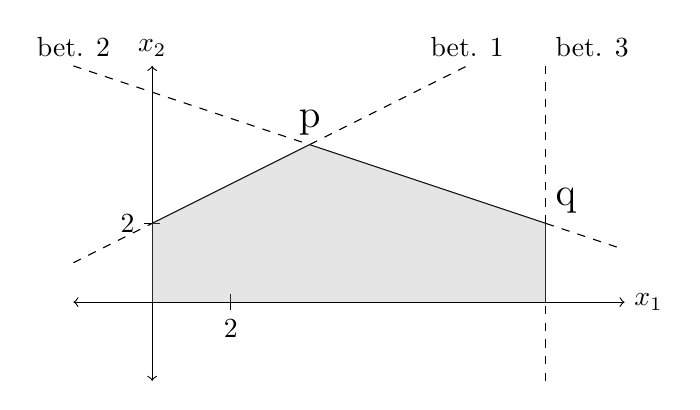
\begin{tikzpicture}
  %laver Grid. godt til når koordinater skal redigeres
  	%\draw[thin,gray!40] (-3,-1) grid (6,3); 
  %x-aksen
  	\draw[<->] (-1,0)--(6,0) node[right]{$x_1$};
  	%\draw[->,red] (2.5,0) -- (2.5,0.5);
  %y-aksen
  	\draw[<->] (0,-1)--(0,3) node[above]{$x_2$};
  	%\draw[->,red] (0,0.5) -- (0.5,0.5);
  	
  %akse-markeringer
  	%\node[left] (xakse) at (0,1) {2};
  	\draw[] (-0.1,1) -- (0.1,1) node[pos=0,left] {2};
  	\draw[] (1,-0.1) -- (1,0.1) node[pos=0,below] {2};
  	
  %ligning 1
	\draw[domain=-1:0,variable=\x,dashed] 	plot({\x},{0.5*\x+1});
	\draw[domain=0:2,variable=\x] 			plot({\x},{0.5*\x+1});
	\draw[domain=2:4,variable=\x,dashed] 	plot({\x},{0.5*\x+1}) node[above] {bet. 1};
  	%\draw[->,red] (1,1.5) -- (1.224,1.05);
	
  %ligning 2
  	\draw[domain=-1:2,variable=\x,dashed] 	plot({\x},{-(1/3)*\x+8/3}) node[above] at (-1,3) {bet. 2} ;
	\draw[domain=2:5,variable=\x] 			plot({\x},{-(1/3)*\x+8/3});
	\draw[domain=5:6,variable=\x,dashed] 	plot({\x},{-(1/3)*\x+8/3});
	%\draw[->,red] (3.5,1.5) -- (3.34,1.026);

  %ligning 3
  	\draw[domain=-1:0,variable=\y,dashed] 	plot({5},{\y});
	\draw[domain=0:1,variable=\y] 			plot({5},{\y});
	\draw[domain=1:3,variable=\y,dashed] 	plot({5},{\y}) node[above right] {bet. 3};
	%\draw[->,red] (5,0.5) -- (4.5,0.5);

  %nodes med navne på punkter
	\node[above] (p) at (2,2) {\Large p};
	\node[above right] (q) at (5,1) {\Large q};

  %løsningsmængden skraveret
	\fill[gray!80,nearly transparent] (0,0) -- (0,1) -- (2,2) -- (5,1) --(5,0) --  cycle;
\end{tikzpicture}
	\captionof{figure}{Løsningsmængde med naboløsninger $p$ og $q$.}
	\label{fig:nabo}
	\end{center}
	
\label{eks:nabo}
\end{eks}

%ved ikke: Må et afsnit slutte med et eksempel?

\section{Optimale løsning}
\label{sec:eksistens}
Hvis løsnings mængden til et lineært programmerings problem ikke er tom, må der være en løsning til problemet.
Men bare fordi der eksistere en løsning, behøver der ikke eksistere en optimal løsning. 
%\begin{defn}
%Lad $P=\{\vec{x} \in \mathds{R}^n| A \vec{x} \geq b, \vec{x} \geq \vec{0}\} \neq \emptyset$ være en polyide, svarende til bibetingelserne til det lineære minimerings problem $\vec{c}^T\vec{x}$.
%Da siges en vektor $\vec{x^*}\in P$ at være \textbf{optimal}, hvis $\vec{c}^T\vec{x^*}\leq \vec{c}^T\vec{x}$ for alle $\vec{x}\in P$
%\end{defn}
Betragt tilfældet, hvor der eksistere en vektor i løsningsmængden, hvor det er muligt at lægge en vilkårlig stor vektor til, og summen stadig er indholdt i løsnings mængden.
Er det tilfældet siges løsningsmængden at indeholde en linje.
\begin{defn}[Linje]
Lad $P\subseteq \mathds{R}^n $ være en polyide, da indeholder $P$ en \textbf{linje}, hvis $\vec{x}+\lambda\vec{d} \in P$ for alle $\lambda \in \mathds{R}^n$, hvor $\vec{x}\in P$ og $\vec{d} \in \mathds{R}^n$.
\end{defn}
Hvis løsningsmængden indholder en linje, så må objektfunktion nødvendigvis kunne tage en vilkårlig stor værdi, og løsningen vil være lig $-\infty$ i tilfældet af, at objektfunktionen skal minimeres. 
Det antyder derfor, at objektfunktionen skal være begrænset, for at der eksistere en optimal løsning.
%\begin{defn} [Begrænset]
%Lad $S \subset \mathds{R}^n$, da er $S$ begrænset, hvis der eksistere en konstant $K$ så $\forall \vec{x} \in S: \langle \vec{x}, \vec{x} \rangle \leq K$
%\end{defn}
Det viser sig, at hvis løsnings mængden ikke er tom og ikke indeholder en linje, så er der en optimal løsning, som vil være en mulig basisløsning, det vil sige, at løsningen findes i et skærings punkt af $n$ lineært uafhængige bibetingelser.
\begin{stn}[Eksistens af optimal løsning]
Lad $P=\{\vec{x} \in \mathds{R}^n| A \vec{x} \geq b \} \neq \emptyset$ være en polyide, svarende til bibetingelserne til det lineære minimerings problem $\vec{c}^T\vec{x}$. Hvis $P$ ikke indeholder en linje, da vil der eksistere en optimal løsning $\vec{x^{**}}$ som er en mulig basisløsning.
\label{stn:eksistens}
\end{stn}
Sætningen bevises med et medføre bevis, ved at finde en vektor $\vec{x}$ i løsningsmængden også konstruere en mulig basisløsning ud fra vektoren. 
Ved at finde en retnings vektor $\vec{d}$, som minimere objektfunktionen, og så lægge et multiplum af $\vec{d}$ til $\vec{x}$ indtil, at summen gør en ny bibetingelse aktiv. 
Det vil altid være muligt at finde sådan en bibetingelse, da løsningsmængden ikke indeholder en linje.
Processen gentages til, vektoren har $n$ lineært uafhængige aktive bibetingelser, se Figur \ref{fig:eksistens}.
\begin{figure}
\begin{center}
	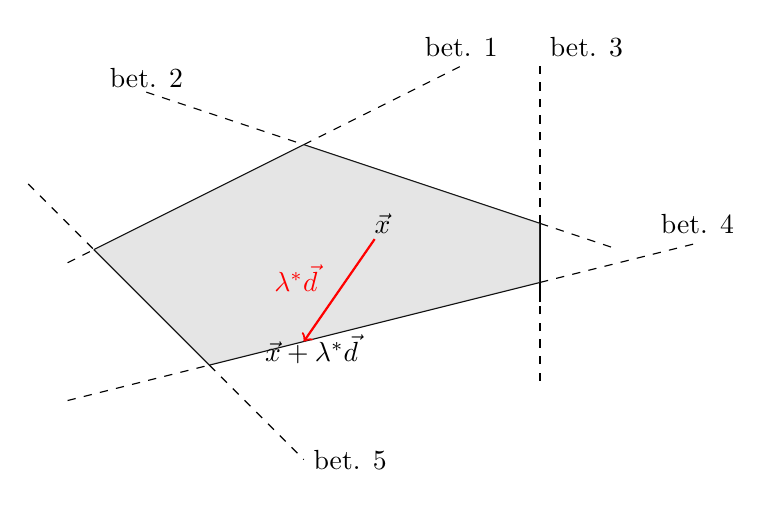
\begin{tikzpicture}[ latex
  s/.style={width=0}]

  %ligning 1
	\draw[domain=-1:-2/3,variable=\x,dashed] 	plot({\x},{0.5*\x+1});
	\draw[domain=-2/3:2,variable=\x] 			plot({\x},{0.5*\x+1});
	\draw[domain=2:4,variable=\x,dashed] 	plot({\x},{0.5*\x+1}) node[above] {bet. 1};
	
  %ligning 2
  	\draw[domain=0:2,variable=\x,dashed] 	plot({\x},{-(1/3)*\x+8/3}) node[above] at (0,2.6) {bet. 2} ;
	\draw[domain=2:5,variable=\x] 			plot({\x},{-(1/3)*\x+8/3});
	\draw[domain=5:6,variable=\x,dashed] 	plot({\x},{-(1/3)*\x+8/3});
	

  %ligning 3
  	\draw[domain=-1:0,variable=\y,dashed] 	plot({5},{\y});
	\draw[domain=0:1,variable=\y] 			plot({5},{\y});
	\draw[domain=1:3,variable=\y,dashed] 	plot({5},{\y}) node[above right] {bet. 3};
	
  %ligning 4
	\draw[domain=-1:4/5,variable=\x,dashed] 	plot({\x},{0.25*\x-1});
	\draw[domain=4/5:5,variable=\x] 			plot({\x},{0.25*\x-1});
	\draw[domain=5:7,variable=\x,dashed] 	plot({\x},{0.25*\x-1}) node[above] {bet. 4};
	
  %ligning 5
  	\draw[domain=-1.5:-2/3,variable=\x,dashed] 	plot({\x},{-\x}) ;
	\draw[domain=-2/3:4/5,variable=\x] 			plot({\x},{-\x});
	\draw[domain=4/5:2,variable=\x,dashed] 	plot({\x},{-\x}) node[right] {bet. 5} ;

  %løsningsmængden skraveret
	\fill[gray!80,nearly transparent] (4/5,-4/5) -- (-2/3,2/3) -- (2,2) -- (5,1) --(5,0.25) --  cycle;
	
  % vektor x
	\node[] (x) at (3,1) {$\vec{x}$};
	\draw[thick, color=red, ->](2.9,0.8) -- (2,-0.5) node[above, yshift=0.5 cm, xshift=-0.1 cm] {$\lambda^* \vec{d}$} ;
	\node[] (x) at (2.1, -0.6) {$\vec{x}+\lambda^* \vec{d}$};
 
\end{tikzpicture}
	\captionof{figure}{Der ligges et multiplum af en retnings vektor til vektor $\vec{x}$ til at summen gør betingelse $4$ aktiv.}
	\label{fig:eksistens}
\end{center}
\end{figure}
Da objektfunktionen til enhver vektor i løsningsmængden, derfor er mindre eller lig objektfunktionen til en mulig basisløsning, må den optimale løsning, være en mulig basisløsning.
\begin{proof}
Da $P$ ikke er tom må der eksistere en vektor $\vec{x} \in P$.
Antag at $\vec{x}$ ikke er en mulig basisløsning, da vil $I = \{i | \vec{a_i}^T\vec{x} = b_i\}$, hvor $\vec{a_i}^T\vec{x}=b_i$ er aktive lineære uafhængige bibetingelser, indeholde færre end $n$ elementer. 
Nu konstrueres en mulig basisløsning $\vec{x^*}$, med udgangspunkt i $\vec{x}$ så $\vec{c}^T\vec{x^*}\leq \vec{c}^T\vec{x}$.
Da $|I|<n $ må $span(\{a_i | i \in I\})$ være et ægte underrum til $\mathds{R}^n$, hvorfor der eksistere en vektor $\vec{d} \in \mathds{R}^n$ så $\vec{a_I}^T\vec{d}=0$ for alle $i \in I$. 
Vælg nu fortegn på $\vec{d}$ så $\vec{c}^T\vec{d} \leq 0$, da vil $\vec{c}^T(\vec{x}+\lambda\vec{d}) \leq \vec{c}^T\vec{x}$ hvor $\lambda$ er en positiv skalar.
Da $P$ er begrænset, og derfor ikke indeholder en linje, må der være et $\lambda'$ som gør, at $\vec{x}+\lambda'\vec{d} \notin P$, hvorfor at der for et $\lambda^*$ må gælde, at $\vec{a_j}^T(\vec{x}+\lambda^* \vec{d}) = b_j$, for $j \notin I$.
Bemærk at $\vec{x}+\lambda^*\vec{d} \in P$, da $\vec{a_i}^T(\vec{x}+\lambda\vec{d})= \vec{a_i}^T\vec{x} = b_i$, for $i \in I$, hvorfor alle aktive bibetingelser stadig er overholdt.
Antag nu at $\vec{d}$ er lineært afhængig af andre bibetingelser end $\vec{a_j}$, da vil $\vec{a_j}$ også være lineært afhæng af dem, hvorfor det følger af Sætning \ref{stn:PQ}, at man kan se bort fra dem, og $\vec{x}+\lambda \vec{d} \in P$ må derfor stadig gøre sig gældende. 
Da $\vec{d}$ er lineært afhængig af $\vec{a_j}$, må det medfører, at da $\vec{d}$ er lineært uafhængig af $\vec{a_i}$ så må $\vec{a_j}$ også være det. 
Derfor kan $j$ tilføjes til $I$. 
Gentag til at $I$ indeholder $n$ lineært uafhængige vektorer, hvorefter det følger af Definition \ref{def:basislosning} at en basisløsning er konstrueret, og da løsningen er konstrueret ud fra en mulig løsning uden at overtræde nogle betingelser, må det være en mulig basisløsning.\\
Da $\vec{x^*}$ er konstrueret ud fra en vilkårlig vektor $\vec{x}\in P$ medføre det, at en mulig basisløsning altid vil opfylde $\vec{c}^T\vec{x^*} \leq \vec{c}\vec{x}$ for en hver ikke mulig basisløsning. 
Da der kun er en endelig mængde mulige basisløsninger, må der være en vektor $\vec{x^{**}}$, som opfylder, at $\vec{c}^T\vec{x^{**}}\leq \vec{c}^T\vec{x^*}$ for alle andre mulige basisløsninger, hvorfor at $\vec{x^{**}}$ er en optimal løsning.
\end{proof}
Sætning \ref{stn:eksistens} kan omskrives en smugle, så i stedet for at kravet er, at løsningsmængden ikke har en linje, så er det at objekt funktionen til løsningsmængden er begrænset.
\begin{kor}
Lad $f(\vec{x}) = \vec{c}^T\vec{x}$ betegne et lineært minimerings programmerings problem, med mulige løsningsmængde $\mathcal{F} \neq \emptyset$. 
Da eksistere en optimal løsning, som er en mulig basisløsning, hvis der eksistere et $K \in \mathds{R}$ så $|f(\mathcal{F})| \leq K$ 
\label{kor:eksistens}
\end{kor}
\begin{proof}
Lad  $K \in \mathds{R}$ så $|f(\mathcal{F})| \leq K$, da må der for et hvert $\vec{x} \in P$ og $\vec{d} \in \mathds{R}^n$ eksistere et $\lambda$ så $f(\vec{x}+\lambda \vec{d}) = K$, og da $f$ er lineær, følger det, at $\mathcal{F}$ ikke kan indeholde en linje. 
Da $\mathcal{F} \neq \emptyset$ følger det af Sætning \ref{stn:eksistens}, at er eksistere en optimal løsning, som er en mulig basisløsning til det lineære minimerings programmerings problem.
\end{proof}
Det betyder, at hvis der til et lineært programmerings problem skal eksistere en optimal løsning, så må løsningsmængden ikke indeholde en linje og objektfunktion på løsningsmængden skal være begrænset. 
Er det ikke tilfældet må objektfunktionen kunne tage værdierne $\infty$ og $-\infty$, og det vil derfor være løsningen på problemet, alt afhængig af om, der er tale om et henholdsvis maksimering eller minimerings problem.





%\endgroup
\chapter{Løsninger til lineær programmeringsproblemer}


\section{Basisløsninger}

%Jeg har endnu ikke fået gennemgået beviserne til de to sætninger ordentligt. de er bare stjålet fra jer andre.

Basisløsninger danner grundlaget for udregningen af den optimale løsning, hvilket beskrives og anvendes i Kapitel \ref{afsnit:simplex}. For at kunne beskrive netop basisløsninger er det nødvendigt først at introducere definitionen for aktive betingelser.%Ved ikke: Skal vi også bruge fed når ord introduceres i bindende tekst?

\begin{defn}[Aktive betingelser]
En betingelse siges at være en \textbf{aktiv betingelse} for en givet løsningsvektor $\vec{x}^*$, hvis det gælder, at\\ $\vec{a}_i^T \vec{x}^* = b_i$.
\label{def:aktiv}
\end{defn}

Generelt bliver aktive betingelser brugt, da de for uligheder repræsenterer en grænse for de mulige løsninger i en given retning, mens de for ligheder blot beskriver, at betingelsen er opfyldt.
Yderligere anvendes skæringen mellem disse aktive betingelser, da den optimale løsning for lineære programmeringsproblemer findes i netop disse skæringer. Hvorfor dette netop er tilfældet bliver begrundet i Afsnit \ref{sec:eksistens}.

\begin{stn}[Lineært uafhængige rækker]
Lad $\vec{x}^* \in \mathds{R}^n$ og $I = \{i | \vec{a_i}^T \vec{x}^* = b_i\}$ være mængden af indekser for aktive betingelser. Da er følgende udsagn ækvivalente:
\begin{enumerate}[label=(\alph*)]
\item Mængden $R_a =\{\vec{a_i}| i\in I\}$ indeholder vektorer, hvoraf $n$ af dem er lineært uafhængige.
\item Spannet $span(R_a) = \mathds{R}^n$.
\item Ligningssystemet $\vec{a_i}^T \vec{x}^* = b_i$, for $i \in I$ har en entydig løsning.
\end{enumerate}
\label{stn:uniklosning}
\end{stn} %Ved ikke: Bør det siges at $\vec{a_i}$ repræcentere en række, eller er det underforstået i rapporten da den altid gør det?

\begin{proof}
	(a) <=> (b): Antag at der i $R_a$ er $n$ lineært uafhængige vektorer. Da der er $n$ lineært uafhængige vektorer må dimensionen af spannet af $R_a$ være $n$. Da $dim(span(R_a))=dim(\mathds{R}^n)=n$ og da $R_a \subseteq \mathds{R}^n$ må det følge af Sætning \ref{stn:dimunderrum} at $span(R_a)=\mathds{R}^n$. Tilsvarende gælder det at hvis $span(R_a)=\mathds{R}^n$, må det gælde at $dim(span(R_a))=dim(\mathds{R}^n)=n$. Da vil kardinaliteten af en basis for $R_a$ nødvendigvis være $n$, hvorved $R_a$ skal indeholde $n$ lineært uafhængige vektorer.


(a) <=> (c): Antag at $span(R_a)=\mathds{R}^n$. Antag nu for modstrid, at der findes to løsninger, $\vec{x}_a$ og $\vec{x}_b$, som opfylder $\vec{a}_i\vec{x}=\vec{b}$ for alle $i \in I$. 
Da vil det for alle $i \in I$ gælde at $\vec{a}_i^T\vec{x}_a=\vec{b}$ og at $\vec{a}_i^T\vec{x}_b=\vec{b}$, hvorved $\vec{a}_i^T\vec{d}=\vec{0}$, hvor $\vec{d}=\vec{x}_a-\vec{x}_b$. 
Vektoren $\vec{d}$ vil da være orthogonal på alle $\vec{a}_i$ for $i \in I$ og kan derfor ikke være en lineær kombination af disse. Herved kan $R_a$ ikke udspænde hele $\mathds{R}^n$, da $\vec{d} \in \mathds{R}^n$ men $\vec{d} \notin span(R_a)$.
Tilsvarende antages det nu at der kun er en unik løsning til ligningssystemet. For modstrid antages det at $R_a$ ikke udspænder hele $\mathds{R}^n$ Der kan derved vælges en vektor $\vec{d}$ som er orthogonal til $span(R_a)$ hvorved $\vec{a}_i^T(\vec{x}+\vec{d})=\vec{b}$. Derved er $\vec{x}$ ikke en unik løsning og der er opstået modstrid.
\end{proof}
	
Nu hvor aktive betingelser og lineært uafhængige rækker er definere, kan basisløsninger definere og beskrives

\begin{defn}[Basisløsning og mulig basisløsning]
Lad $P$ være et polyeder dannet af lineære bibetingelser, og lad $\vec{x}^*\in \mathds{R}^n$. Da er $\vec{x}^*$ en \textbf{basisløsning}, hvis
\begin{enumerate}[label=(\alph*)]
\item Alle lighedskrav er aktive
\item Af de aktive betingelser er $n$ lineært uafhængige
\end{enumerate}
og en \textbf{mulig basisløsning}, hvis
\begin{enumerate}[label=(\alph*)]
\setcounter{enumi}{2}
\item hvis $\vec{x}^* \in P$ er en basisløsning.
\end{enumerate}
\label{def:basislosning}
\end{defn}
Det vil sige at en basisløsning ikke nødvendigvis ligger ikke i løsningsmængden, da skæringen mellem de $n$ lineært uafhængige krav ikke pr. Definition \ref{def:basislosning} behøver at ligge i løsningsmængden, og en mulig basisløsning er dermed det særtilfælde af basisløsninger som tilhører løsnings mængden.
En konsekvens af at en basisløsning altid skal have $n$ lineært uafhængige aktive betingelser er, i følge Sætning \ref{stn:uniklosning}, er at basisløsningen er en entydig løsning til ledningssystemet af de $n$ aktive bibetingelser.
%der skal måske lige laves en merge her
%Enhver bibetingelse udspænder et rum, for hvilket betingelsen er opfyldt. Skæringen, af de aktive betingelser, danner derved et rum, som er fællesmængden af betingelsernes udspændte rum. Skæringen, af en mængde af aktive betingelser, svarer derved til den mulige mængde af disse betingelser. Dog gælder det for basisløsninger pr. Definition \ref{def:basislosning}, at der for en basisløsning $\vec{x}$ skal være $n$ lineært uafhængige aktive betingelser, hvorved en basisløsningen er en unik vektor, hvilket er bevist igennem Sætning \ref{stn:uniklosning}. %Ved ikke, er en vektor og et punkt det samme?

\begin{kor}[Endelig mængde af basisløsninger]
Givet en endelig mængde af bibetingelser, vil der kun eksistere en endelig mængde af basisløsninger og derved også kun en endelig mængde mulige basisløsninger.
\label{kor:endeligbasis}
\end{kor}

\begin{proof}
Betragt et lineært ligningssystem med $m$ uligheder og løsningsvektorer på formen $\vec{x} \in \mathds{R}^n$, hvor m er et endeligt tal.
	Betragt da systemet af $n$ aktive uafhængige lineære uligheder udvalgt af de $m$ uligheder. Da vil dette system ifølge Sætning \ref{stn:uniklosning} kun have en løsning, og denne udvælgelse af uligheder giver derved kun en basisløsning. Da der kun er en endelig mængde af muligheder for at udtrække $n$ af $m$ uligheder på, vil der netop også kun være en endelig mængde af basisløsninger. Da mængden af mulige basisløsninger er en delmængde af mængden af basisløsninger, vil der også kun være en endelig mængde af mulige basisløsninger.
\end{proof}

Det at en basisløsning er en entydig løsning til ligningssystemet af dens $n$ lineært uafhængige bibetingelser kan bruges til at finde en procedure til at finde basisløsninger.

\begin{stn}[Krav til basisløsninger]
Lad $A\vec{x}=\vec{b}$ og $\vec{x}\geq 0$, hvor $A$ er en $m\times n$ matrix med lineært uafhængige rækker. Da er $\vec{x}^*\in \mathds{R}^n$ en basisløsning hvis og kun hvis $A\vec{x}^*=b, \vec{x}^* \geq 0$, og der eksisterer indekser $B(1), ..., B(m)$ således, at
\begin{enumerate}[label=(\alph*)]
\item Kolonerne $A_{B(1)}, ..., A_{B(m)}$ er lineært uafhængige og
\item $x_j = 0$, hvis $j \neq B(1),...,B(m)$.
\end{enumerate}
\label{stn:kravtilbasis}
\end{stn}

\begin{proof}
Først vises at (a) og (b) medfører at $\vec{x}$ er en basisløsning.
Lad $I_m$ være mængden af indeks for de lineært uafhængige søjler  $I_m=\{B(1),\dots,B(m)\}$. Per definition er $\vec{b}=\sum_{j=1}^{n} x_j \vec{A}_j$, hvilket må være det samme som $\vec{b}=\sum_{j\in I_m} x_j \vec{A}_j+\sum_{j\notin I_m} x_j \vec{A}_j$, hvor summeringen er opdelt efter om kolonnerne har indeks $i \in I_m$. 
Ifølge sætningens punkt (b) er $x_j=0$ for $j \notin I_m$. Derved bliver summeringen forkortet til $\vec{b}=\sum_{j\in I}x_j \vec{A}_j$. Da vektorerne $\vec{A}_j$ for $j \in I_m$ er lineært uafhængige vil ligningssystemet nødvendigvis have en unik løsning. Da ligningssystemet har en unik løsning gælder det af Sætning \ref{stn:uniklosning}, at ligningssystemet har $n$ lineært uafhængige rækker, som alle er aktive. Da der er $n$ aktive betingelser og da alle lighedskrav er aktive, vil det pr. Definition \ref{def:basislosning} sige at $\vec{x}$ er en basisløsning.

% som er summen af alle de lineære uafhængige rækker og deres løsninger lagt sammen med summen af de lineære afhængige rækker og deres løsninger, men $\vec{x_j}$ til de lineære uafhængige løsninger er er i følge sætningen $x_i = 0$ hvis $i \neq B(1),...,B(m)$ så derfor må ligningen blive $b=\sum_{j\in I_m}^{n}x_j \vec{A}_j+0$,
% 
%så derfor må $\vec{x}$ være en basis løsning.

Herefter vises at det at $\vec{x}$ er en basisløsning medfører (a) og (b). Antag at $\vec{x}$ er en basisløsning og lad $x_j$ for indekser $j \in I_k=\{B(1),\dots B(k)\}$ være alle ikke-nul komponenter af $\vec{x}$.
Eftersom $\vec{x}$ er en basisløsning, så må ligningssystemet af aktive betingelser $\sum_{j=1}^{n}\vec{A}_jx_j=\vec{b}$, hvor $x_j=0$ for $j\notin I_k$ have en unik løsning. Dette gælder da en basisløsning har $n$ lineært uafhængige aktive betingelser, hvilket ifølge Sætning \ref{stn:uniklosning} medfører at systemet har en unik løsning. 
Ligeledes må ligningen $\sum_{j \in I_k}\vec{A}_jx_j=\vec{b}$ have en unik løsning og derfor må kolonerne $\vec{A}_{B(1)}, ..., \vec{A}_{B(k)}$ være lineært uafhængige. Derfor må det gælde at $k \leq m$. % Hvis ikke dette var tilfældet ville der eksistere flere $\vec{x}$ som opfylder ligningssystemet, hvilket modstrider at der er en unik løsning.\\
%Eftersom kolonerne $\vec{A}_{B(1)}, ..., \vec{A}_{B(k)}$ er lineært uafhængige, så må det gælde at $k\leq m$. 
Da $A$ har $m$ lineært uafhængige rækker, må $A$ også have $m$ lineært uafhængige kolonner, hvorved $Col(A)=\mathds{R}^m$.

Den næste del af beviset viser, at der for enhver udvælgelse af indekser $I_k$ findes indekser $I_m$ således at $I_k \subseteq I_m$. 
%Den næste del af beviset viser, at der for enhver udvælgelse af $k$ lineært uafhængige kolonner med indekser $I_k$, gælder at der findes en mængde af $m$ lineært uafhængige kolonner med indekser $I_m$, hvorom det gælder at $I_k \subseteq I_m$.
Altså findes der indekser $B(k+1),...,B(m)$, således at kolonnerne med indekser $B(1),...,B(k),...,B(m)$ er lineært uafhængige. 

Hvis alle $\vec{A}_j$ for $j \notin I_k$ er lineært afhængige af $\vec{A}_j$ for $j \in I_k$, gælder det at $span\left( \vec{A}_{B(1)},...,\vec{A}_{B(k)} \right)=Col(A)=\mathds{R}^m$, hvorved $k=m$. 
Hvis der i stedet eksisterer en kolonne med indeks $j \notin I_k$ som er lineært uafhængig af disse kolonner, kan denne tilføjes til mængden af nu $k+1$ uafhængige vektorer. Denne proces kan gentages $m-k$ gange. Da $i \notin I_m$ medfører at $i \notin I_k$ gælder det derved at $\vec{x}_i =0$ for $i \notin I_m$
\end{proof}

\begin{pro}{Procedure for konstruktion af basisløsninger}
Vælg $m$ lineært uafhængige koloner $\vec{A}_{B(1)},\dots,\vec{A}_{B(m)}$
Lad $x_i=0 \,\forall i\neq B(1),\dots,B(m)$
Løs $A\vec{x}=\vec{b}$ for de ubekendte $x_{B(1)},\dots x_{B(m)}$
\end{pro}
Bemærk at proceduren indirekte kan bruges til at finde mulige basisløsninger, da de er et særtilfælde af basisløsninger.\\
%En Basis løsning lavet med denne procedure, så længde den ikke er negativ, kaldes den for en mulig basisløsning. Og fordi en mulig basisløsning er en basisløsning, så kan en mulig basisløsning findes, ved at lave basisløsninger.\\

Hvis $\vec{x}$ er en basisløsning, kaldes indgangene $x_{B(1)},\dots ,x_{B(m)}$ for basis variable, mens $x_i \,\forall i\neq B(1),\dots,B(m)$ kaldes for ikke-basis variabler. Mens søjlerne $\vec{A}_{B(1)},\dots,\vec{A}_{B(m)}$ udgør en basis for $\mathds{R}^m$ ifølge Sætning \ref{stn:uniklosning}.
\begin{defn}
Lad $\vec{x}$ en basisløsning så $x_i = 0$ for alle $i \notin I_B$, da er $B = [\vec{A_i}: i \in I_B]$ \textbf{basismatricen} knyttet til basisløsningen. 
Og ved $\vec{x}_B$ forstås løsningen til ligningsstemmet $B\vec{x}_B =\vec{b}$.
\end{defn}
Bemærk at da $B$ består af $m$ lineært uahængige rækker og er en $m\times m$ matrix følger det af Sætning \ref{stn:inversmatrix}, at $B^{-1}$ eksistere. 


%\\ %måske et andet ord
%Søjlerne $A_{B(1)},\dots ,A_{B(m)}$ kaldes for basis søjlerne og da de er lineært uafhængige, så danne de en basis for $\mathds{R}^m$\\
%To baser kan være forskellige, men de vil blive betragtet som værende to forskellige mængder $\{B(1),\dots,B(m)\}$ af basis indekser, hvis disse to mængde består af de samme basis indekser, så vil de blive betragtet som værende samme basis.\\
%Hvis søjlerne $\vec{A}_{B(1)},\dots,\vec{A}_{B(m)}$, bliver sat ved siden af hinanden, så der dannes $m\times m$ matrixen $B$, som kaldes en basis matrix. ligeledes dannes vektoren $\vec{x}_{B}$ bestående af basis variablerne. Basis variablerne er bestemt ved at løse ligningen $B\vec{x}_B=\vec{b}$ således at en unik løsning er givet ved $\vec{x}_B=B^{-1}\vec{b}$
%\begin{defn}
%Betragt en $m\times m$ basis matrix $B$ dannet af lineært uafhængige søjler fra $A$ i $A\vec{x}=\vec{b}$
%
%\end{defn}

\begin{comment}
Der mangler bare generelt bindetekst mellem sætninger, fra at korollar 6.12 skal introduceres til at kapitlet skal afsluttes og føres videre til naboløsninger
\end{comment}





\subsection{Naboløsninger}

Til den senere anvendelse af simplex metoden anvendes også \textbf{naboløsninger}, som er defineret i Definition \ref{def:nabo}. Undersøgelsen af naboløsninger i simplex metoden som en metode til at reducere antallet af basisløsninger, som skal undersøges når den optimale løsning findes. %Bør omformuleres, er kringlet. Ved ikke: Er det realt det der sker? Ved ikke: Skal SimpLeX staves med stort? Jeg tror da det er det der sker. og simplex er med lille. hermed rettet.

\begin{defn}[Naboløsninger]
	To basisløsninger i $\mathds{R}^n$ siges af være \textbf{naboløsninger}, hvis de deler præcis $n-1$ aktive lineært uafhængige bibetingelser.
	\label{def:nabo}
\end{defn}

Et eksempel på naboløsninger ses i Eksempel \ref{eks:nabo}.

\begin{eks}[Naboløsninger]
De to basisløsninger $\vec{p}=\rvect{4 & 4}^T$ og $\vec{q}=\rvect{10 & 2}^T$ set på Figur \ref{fig:nabo} er naboløsninger, da de har $n-1$ fælles aktive betingelser, hvilket for dette eksempel er $1$ betingelse, nemlig betingelse (2). Basisløsningen $\vec{p}$ har (1) og (2) som aktive betingelser, mens $\vec{q}$ har (2) og (3) som aktive betingelser. %ved ikke, om nemlig bør slettes.
	
	\begin{center}
	\begin{tabular}{l	>{$}r<{$}	>{$}r<{$}	>{$}l<{$} r}
	Maksimer 		& 		4x_1	&	+3 x_2	& \\
	med hensyn til 	&  \ \ 	-2 x_1	& 	+4 x_2	& \leq 8 	& \quad (1)\\
					&  		x_1		& 	+3 x_2	& \leq 16	& \quad (2)\\
					&  \ \ 	x_1		& 			& \leq 10	& \quad (3)\\
	og $x_1 \geq 0$ (4), $x_2\geq 0$ (5).
	\end{tabular}
	\end{center}
	
	\begin{center}
	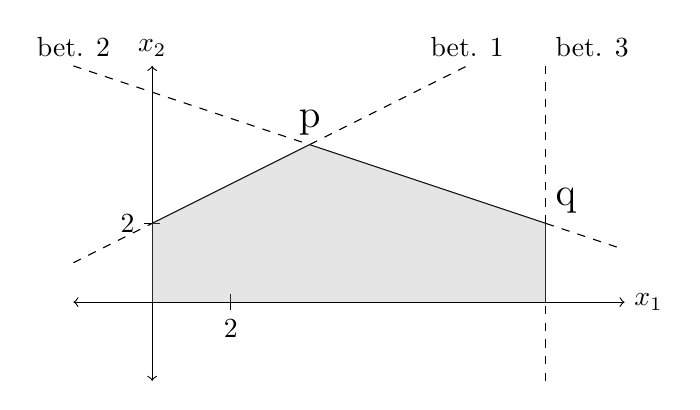
\begin{tikzpicture}
  %laver Grid. godt til når koordinater skal redigeres
  	%\draw[thin,gray!40] (-3,-1) grid (6,3); 
  %x-aksen
  	\draw[<->] (-1,0)--(6,0) node[right]{$x_1$};
  	%\draw[->,red] (2.5,0) -- (2.5,0.5);
  %y-aksen
  	\draw[<->] (0,-1)--(0,3) node[above]{$x_2$};
  	%\draw[->,red] (0,0.5) -- (0.5,0.5);
  	
  %akse-markeringer
  	%\node[left] (xakse) at (0,1) {2};
  	\draw[] (-0.1,1) -- (0.1,1) node[pos=0,left] {2};
  	\draw[] (1,-0.1) -- (1,0.1) node[pos=0,below] {2};
  	
  %ligning 1
	\draw[domain=-1:0,variable=\x,dashed] 	plot({\x},{0.5*\x+1});
	\draw[domain=0:2,variable=\x] 			plot({\x},{0.5*\x+1});
	\draw[domain=2:4,variable=\x,dashed] 	plot({\x},{0.5*\x+1}) node[above] {bet. 1};
  	%\draw[->,red] (1,1.5) -- (1.224,1.05);
	
  %ligning 2
  	\draw[domain=-1:2,variable=\x,dashed] 	plot({\x},{-(1/3)*\x+8/3}) node[above] at (-1,3) {bet. 2} ;
	\draw[domain=2:5,variable=\x] 			plot({\x},{-(1/3)*\x+8/3});
	\draw[domain=5:6,variable=\x,dashed] 	plot({\x},{-(1/3)*\x+8/3});
	%\draw[->,red] (3.5,1.5) -- (3.34,1.026);

  %ligning 3
  	\draw[domain=-1:0,variable=\y,dashed] 	plot({5},{\y});
	\draw[domain=0:1,variable=\y] 			plot({5},{\y});
	\draw[domain=1:3,variable=\y,dashed] 	plot({5},{\y}) node[above right] {bet. 3};
	%\draw[->,red] (5,0.5) -- (4.5,0.5);

  %nodes med navne på punkter
	\node[above] (p) at (2,2) {\Large p};
	\node[above right] (q) at (5,1) {\Large q};

  %løsningsmængden skraveret
	\fill[gray!80,nearly transparent] (0,0) -- (0,1) -- (2,2) -- (5,1) --(5,0) --  cycle;
\end{tikzpicture}
	\captionof{figure}{Løsningsmængde med naboløsninger $p$ og $q$.}
	\label{fig:nabo}
	\end{center}
	
\label{eks:nabo}
\end{eks}

%ved ikke: Må et afsnit slutte med et eksempel?
\subsection{Degenererede basisløsninger}
En basisløsning skal have $n$ aktive lineært uafhængige bibetingelser i følge Definition \ref{def:basislosning} (b), det udelukker ikke at en basisløsning kan have flere aktive krav, hvis nogle af kravende er lineært afhængige. 
\begin{defn}[Degenereret basisløsning]
En basisløsning $\vec{x}\in \mathds{R}^n$ siges at være en \textbf{degenereret basisløsning}, hvis basisløsningen har mere en $n$ aktive bibetingelser.
\end{defn}
Det vil sige, at for $\vec{x}\in \mathds{R}^2$, vil $\vec{x}$ være degenereret, hvis $\vec{x}$ ligger på et skæringspunkt af $3$ bibetingelser.
Af Sætning \ref{stn:PQ} følger det, at antagelsen om, at alle bibetingelser er lineært uafhængige ikke ændre løsningsmængden, derfor vil denne rapport kun meget overfladisk nævne degenererede løsninger. 
Men da degenerede løsninger kan give nogle problematikker senere i Simplex metoden, så den terminerer for tidligt, defineres degenererede basisløsninger, for at vise en forståelse for emnets eksistens.
Helt generelt gælder der for basisløsninger til et polyeder på standard form med ligheder, at der altid vil $m$ lighedsbetingelser  aktive. Derfor må, det at have mere end $n$ aktive bibetingelser, betyde at mere end $n-m$ variabler er $0$
\begin{defn}
Lad $P =\{ \vec{x} \in \mathds{R}^n \mid A \vec{x} = \vec{b}, \, \vec{b}\in \mathds{R}^m\}$ være et polyeder på standard form med ligheder, og lad $\vec{x}$ være en basisløsning. Lad $m$ være mængden af rækker i $A$. Så er $\vec{x}$ en degenereret basisløsning, hvis mere end $n-m$ komponenter af $\vec{x}$ er $0$.
\end{defn}


%I følge af definition \ref{def:basislosning} (b) skal en basis løsning, bare have $n$ lineære uafhængige aktive betingelser i $\mathds{R}^n$, dette giver muligheden for, at der er mere end $n$ aktive betingelser (Der kan selvfølge i $\mathds{R}^n$ ikke være mere end $n$ lineære uafhængige aktive betingelser). Sådan en basisløsning kaldes for en Degenereret basisløsning. Der vil i denne rapport, ikke blive arbejdet med degenereret basisløsninger, da der menes at rapports indhold i forvejen er tilstrækkeligt, dette kan komme til at give nogle problematikker senere i Simplex-metoden, der for den til at terminere for tidligt, så derfor defineres degenereret basisløsninger, for at vise en forståelse for emnet eksistens.
%\begin{defn}[Degenereret basisløsning]
%En basisløsning $\vec{x}\in \mathds{R}^n$ siges at være en \textbf{Degenereret basisløsning}, hvis basisløsningen har mere en $n$ aktive betingelser
%\end{defn}

%Det vil sige, at for $\vec{x}\in \mathds{R}^2$, vil $\vec{x}$ være degenereret, hvis $\vec{x}$ ligger på et skæringspunkt af $3$ betingelser.
%\textit{måske et eksempel}\\
%\subsubsection{Degenereret basisløsninger i standard form}
%En basisløsning til en polyede på standard form, vil $m$ lighedsbetingelser altid være aktive. Derfor må, at have mere end $n$ aktive betingelser, være at mere end $n-m$ variabler er $0$
%\begin{defn}
%En polyede på standard form $P =\{ \vec{x} \in \mathds{R}^n | A \vec{x} = \vec{b}, \vec{b}\in \mathds{R}^m\}$ og lad $\vec{x}$ være en basisløsning. Lad $m$ være mængden af rækker i $A$. Så er $\vec{x}$ en degenereret basisløsning, hvis mere end $n-m$ komponenter af $\vec{x}$ er $0$
%\end{defn}
%Dette vil dog næsten ikke ske, hvis komponenterne af $A$ og $\vec{b}$ er valgt tilfældigt.
%Det der sker er, at når der bliver valgt $m$ rækker af $A$ som danner basis og $m$ variabler bliver udregnet til en basisløsning, så opfylder denne løsning også et andet krav, og derfor vil der under rækkeoperationerne resultere i, at en af de valgte variabler bliver $0$
\section{Eksistens af en optimale løsning}
\label{sec:eksistens}
Hvis det lineære programmeringsproblem er konsistent, betyder det, at der er en løsning til det, men bare fordi der er en løsning, betyder det ikke, at der er en optimal løsning.
Hvis der skal eksistere en optimal løsning, må løsningsmængden ikke indeholde en linje.
%\begin{defn}[Linje]
%Lad $P\subseteq \mathds{R}^n $ være et polyeder, da indeholder $P$ en \textbf{linje}, hvis $\vec{x}+\lambda\vec{d} \in P$ for alle $\lambda \in \mathds{R}_+$, hvor $\vec{x}\in P$ og $\vec{d} \in \mathds{R}^n$. Hvis $\vec{x}+\lambda\vec{d} \in P$ for $\lambda > 0$ eller $\lambda < 0$, siges $P$ at indeholde henholdsvis en positiv eller negativ halv linje.
%
%\end{defn}

\begin{defn} [Linje]
Lad $P\subseteq \mathds{R}^n $ være et polyeder og $\vec{x} \in P$, da indeholder $P$ ikke en \textbf{positiv halvlinje}, hvis $\forall \vec{d} \in \mathds{R}^n \nexists \lambda \in \mathds{R}_+ : \vec{x}+\lambda \vec{d} \in P$, og indeholder ikke en \textbf{linje} hvis $\forall \vec{d} \in \mathds{R}^n \nexists \lambda \in \mathds{R} : \vec{x}+\lambda \vec{d} \in P$.
\label{def:linje}
\end{defn}

Det betyder, at der til en løsning i polyederet kan lægges en retningsvektor til.
Denne retningsvektor bliver skaleret, så løsningen nu ligger et andet sted. 
Hvis der findes en retning, hvor det resulterer i at løsning stadig er i polyeden, selvom $\lambda$ er vilkårligt stor, så siges polyederet at have en linje.
%Det betyder, at der til en løsning kan lægges et vilkårligt stort multiplum af en vektor til, og summen vil stadig være en løsning, derfor må objektfunktionen nødvendigvis også kunne tage en vilkårlig stor værdi.
\begin{prop}
Lad løsningsmængden $P = \{ \vec{x} \in \mathds{R}^n\mid A \vec{x} \geq \vec{b} \} \subseteq \mathds{R}^n $  til det lineære minimeringsproblem $\vec{c}^T\vec{x}$, indeholde en linje
\begin{align*}
\vec{x} + \lambda \vec{d}, \quad \vec{d}\in \mathds{R}^n, \, \vec{c}^T\vec{x} \neq 0, \, \lambda \in \mathds{R}.
\end{align*}
Da er den optimale værdi $-\infty$.
\end{prop}
\begin{proof}
Da $P$ indeholder en linje, følger det af Definition \ref{def:linje}, at der eksistere en vektor $\vec{x} \in P$ og en vektor $\vec{d} \in \mathds{R}^n$, så $\vec{x}+\lambda \vec{d} \in P$, for alle $\lambda \in \mathds{R}^n$. 
Fordi $\vec{c}^T\vec{d}\neq 0$, medfører det, at $\lambda$ kan vælges så $\vec{c}^T(\vec{x}+\lambda\vec{d}) = - \infty$, hvorfor den optimale værdi må være $-\infty$.
\end{proof}
Bemærk, at da løsningsmængden indeholder en linje, kan løsningsmængden ikke være tom, er løsningsmængden tom, er problemet inkonsistent, og der eksistere derfor ikke en optimal løsning. 
Er løsningsmængden ikke tom, og uden linjer, da eksistere der en optimal løsning, som viser sig at være en mulig basisløsning.
\begin{stn}[Eksistens af en optimal løsning]
Hvis løsningsmængden $P =\{\vec{x} \in \mathds{R}^n\mid A \vec{x} \geq \vec{b} \} \neq \emptyset$, til det lineære minimeringsproblem $\vec{c}^T\vec{x}$, ikke indeholder en positiv halvlinje, da vil der eksistere en optimal løsning $\vec{x}^{**}$, som er en mulig basisløsning.
\label{stn:eksistens}
\end{stn}
\begin{proof}
Antag, at $\vec{x} \in P$ ikke er en mulig basisløsning, og lad $I =\{i \mid \vec{a_i}^T\vec{x}=b_i\}$ betegne indeksene for de lineært uafhængige aktive bibetingelser knyttet til løsningen $\vec{x}$.
Da $\vec{x}$ ikke er en mulig basisløsning, må $span(\{\vec{a_i}\mid i\in I\})$ være et ægte underrum til $\mathds{R}^n$, hvormed det følger af Sætning \ref{stn:Rnorto}, at der eksisterer en vektor $\vec{d} \in \mathds{R}^n$, så $\vec{a_i}^T\vec{d}=0$ for $i \in I$.
Da må $\vec{a_i}^T(\vec{x}\pm \vec{d})= \vec{a_i}^T\vec{x}=b_i$.
Vælg nu fortegn på $\vec{d}$ så $\vec{c}^T\vec{d}\leq 0$, da må $\vec{c}^T(\vec{x}+\lambda\vec{d}) \leq \vec{c}^T\vec{x}$ for en vilkårlig skalar $\lambda > 0$.
Da løsningsmængden ikke indeholder en positiv halvlinje, vil der være en øvre grænse for $\lambda$, før $\vec{x}+\lambda\vec{d} \notin P$, svarende til $\lambda$et, der opfylder $\vec{a_j}^T(\vec{x}+\lambda\vec{d})=b_j$, hvor $\vec{a_j} \notin \{\vec{a_i}\mid i\in I\}$ er den første bibetingelse, der bliver aktiv, se Figur \ref{fig:eksistens}.
Da $\vec{a_i}^T\vec{d}=0$ og $\vec{a_j}^T\vec{d} \neq 0$ medfører det, at $\vec{a_i}$ og $\vec{a_j}$  er lineært uafhængige af Lemma \ref{lma:ortolinuaf}. 
Derfor kan $j$ tilføjes til $I$.
Gentag til at $|I|=n$.
\\ Antag nu, at $|I|=n$, derfor må $\vec{x}$ have $n$ aktive bibetingelser.
Da $\vec{x}\in \mathcal{F}$ medfører det, at $\vec{x}$ overholder alle ligheds bibetingelser, og at $\vec{x}$ er en mulig løsning. 
Derfor følger det af Definition \ref{def:basislosning}, at $\vec{x}$ er en mulig basisløsning.
\\Derfor må der fra en vilkårlig løsning $\vec{x}\in \mathcal{F}$ kunne konstrueres en mulig basisløsning $\vec{x^*}$ så $\vec{c}^T\vec{x^*} \leq \vec{c}^T \vec{x}$.
Dermed må den optimale løsning være den mulige basisløsning, der minimere objektfunktionen, hvorfor der eksistere en optimal løsning, som er en mulig basisløsning.
\end{proof}
\begin{figure}
\begin{center}
	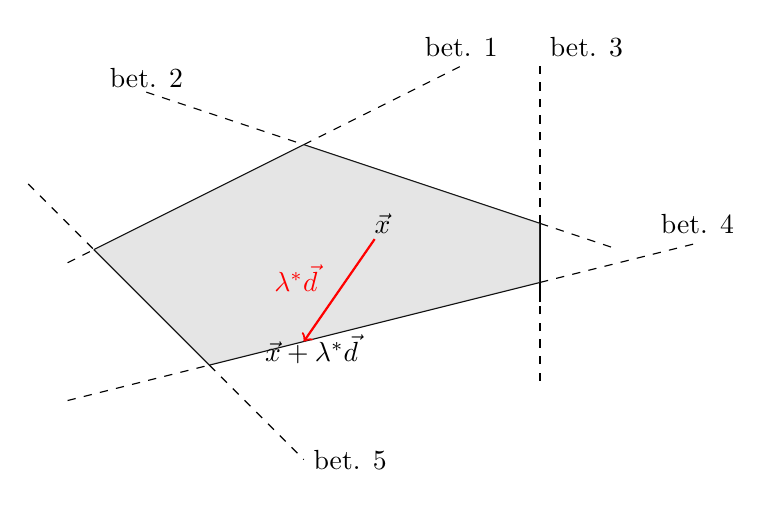
\begin{tikzpicture}[ latex
  s/.style={width=0}]

  %ligning 1
	\draw[domain=-1:-2/3,variable=\x,dashed] 	plot({\x},{0.5*\x+1});
	\draw[domain=-2/3:2,variable=\x] 			plot({\x},{0.5*\x+1});
	\draw[domain=2:4,variable=\x,dashed] 	plot({\x},{0.5*\x+1}) node[above] {bet. 1};
	
  %ligning 2
  	\draw[domain=0:2,variable=\x,dashed] 	plot({\x},{-(1/3)*\x+8/3}) node[above] at (0,2.6) {bet. 2} ;
	\draw[domain=2:5,variable=\x] 			plot({\x},{-(1/3)*\x+8/3});
	\draw[domain=5:6,variable=\x,dashed] 	plot({\x},{-(1/3)*\x+8/3});
	

  %ligning 3
  	\draw[domain=-1:0,variable=\y,dashed] 	plot({5},{\y});
	\draw[domain=0:1,variable=\y] 			plot({5},{\y});
	\draw[domain=1:3,variable=\y,dashed] 	plot({5},{\y}) node[above right] {bet. 3};
	
  %ligning 4
	\draw[domain=-1:4/5,variable=\x,dashed] 	plot({\x},{0.25*\x-1});
	\draw[domain=4/5:5,variable=\x] 			plot({\x},{0.25*\x-1});
	\draw[domain=5:7,variable=\x,dashed] 	plot({\x},{0.25*\x-1}) node[above] {bet. 4};
	
  %ligning 5
  	\draw[domain=-1.5:-2/3,variable=\x,dashed] 	plot({\x},{-\x}) ;
	\draw[domain=-2/3:4/5,variable=\x] 			plot({\x},{-\x});
	\draw[domain=4/5:2,variable=\x,dashed] 	plot({\x},{-\x}) node[right] {bet. 5} ;

  %løsningsmængden skraveret
	\fill[gray!80,nearly transparent] (4/5,-4/5) -- (-2/3,2/3) -- (2,2) -- (5,1) --(5,0.25) --  cycle;
	
  % vektor x
	\node[] (x) at (3,1) {$\vec{x}$};
	\draw[thick, color=red, ->](2.9,0.8) -- (2,-0.5) node[above, yshift=0.5 cm, xshift=-0.1 cm] {$\lambda^* \vec{d}$} ;
	\node[] (x) at (2.1, -0.6) {$\vec{x}+\lambda^* \vec{d}$};
 
\end{tikzpicture}
	\captionof{figure}{Der ligges et multiplum af en retnings vektor til vektor $\vec{x}$ til at summen gør betingelse $4$ aktiv.}
	\label{fig:eksistens}
\end{center}
\end{figure}
Det betyder at hvis det lineære programmerings problem er konsistent, da eksistere der enten en optimal løsning, blandt basisløsningerne eller den optimale løsning er $\pm \infty$.
Det kunne derfor være relevant at finde en måde, hvor den optimale løsning blandt basisløsningerne kan findes, her kan gøres brug af simplex metoden.




\subsection{Lokal optimal løsning}
Når først en optimal løsning er fundet, er det nødvendigt at tjekke, at der ikke er tale om en lokal optimal løsning.
\begin{defn}[Lokalt optimal løsning]
Lad $\vec{x} \in P$ være en løsnings til et minimeringsproblem med objektfunktion $f$, da er $\vec{x}$ en \textbf{lokal optimal løsning}, hvis der for en naboløsning $\vec{y}$ gælder, at $f(\vec{x}) \leq f(\vec{y})$ for $|\vec{y}-\vec{x}|< \epsilon$ for et $\epsilon > 0$ og $\vec{y} \in P$.
\end{defn}
Betragt beviset for Sætning \ref{stn:eksistens}, her konstrueres hele tiden en mere optimal løsning end den foregående, ved at lægge et multiplum af en retningsvektor til den originale vektor, så en ny betingelse blev aktiv.
Der vil derfor kunne opstå et lokalt minimum, hvis der ikke eksistere en sådan retningsvektor, men der er en løsning som er mere optimal, se Figur \ref{fig:lokaltmin}.
\begin{figure}
\begin{center}
	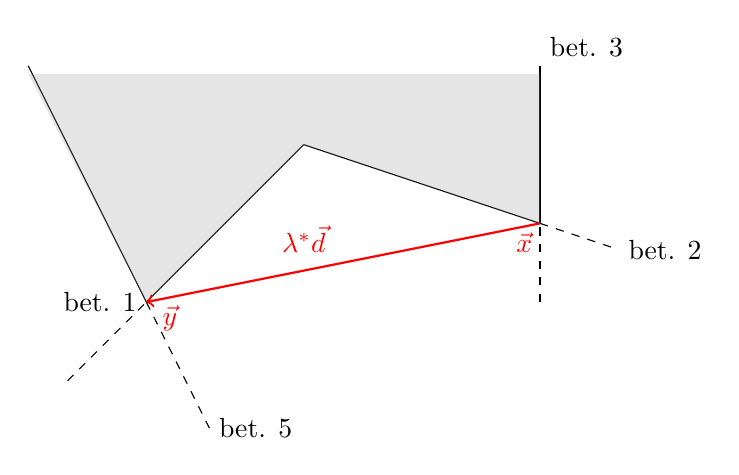
\begin{tikzpicture}[ latex
  s/.style={width=0}]

  %ligning 1
	\draw[domain=-1:0,variable=\x,dashed] 	plot({\x},{\x})  node[left] {bet. 1};
	\draw[domain=0:2,variable=\x] 			plot({\x},{\x});

	
  %ligning 2
	\draw[domain=2:5,variable=\x] 			plot({\x},{-(1/3)*\x+8/3});
	\draw[domain=5:6,variable=\x,dashed] 	plot({\x},{-(1/3)*\x+8/3}) node[right] {bet. 2};
	

  %ligning 3
	\draw[domain=0:1,variable=\y, dashed] 			plot({5},{\y});
	\draw[domain=1:3,variable=\y] 	plot({5},{\y}) node[above right] {bet. 3};
	

	
  %ligning 5
  	\draw[domain=-1.5:0,variable=\x] 	plot({\x},{-2*\x}) ;
	\draw[domain=-0:4/5,variable=\x, dashed] 			plot({\x},{-2*\x}) node[right] {bet. 5} ;


  %løsningsmængden skraveret
	\fill[gray!80,nearly transparent]  (0,0) -- (2,2) -- (5,1) -- (5,2.9) --(-1.5,2.9) --  cycle;
	
  % vektor x
  \node[thick, color=red] (x) at (4.8,0.75) {$\vec{x}$};
  
\node[thick, color=red] (y) at (0.3,-0.2) {$\vec{y}$};
%   %\node[s] (d) at (2, -0.5);
 \draw[thick, color=red, ->](5,1) -- (0,0) node[above, yshift=0.5 cm, xshift=2 cm] {$\lambda^* \vec{d}$} ;
%   \node[] (x) at (2.1, -0.6) {$\vec{x}+\lambda^* \vec{d}$};
%  % \path (x) edge node[right] {$\vec{x}+\lambda^* \vec{d}$} (d) ;
 
\end{tikzpicture}
	\captionof{figure}{Bemærk at der ikke eksistere en retningsvektor $\vec{d}$, så der kan konstueres en bedre løsning, uden at overskride betingelse $2$, derfor vil løsningsvektor $\vec{x}$ fremstå optimal, selvom at løsningsvektor $\vec{y}$ er mere optimal. Løsningsvektor $\vec{x}$ er et lokalt minimum.}
	\label{fig:lokaltmin}
\end{center}
\end{figure}
Det er dog ikke alle mængder, hvor der kan forekomme lokale optimale løsninger, ved fremgangsmåden fra beviset for Sætning \ref{stn:eksistens}.
\begin{defn} [Konveks mængde]
Lad $S \subset \mathds{R}^n$  da er $S$ konveks, hvis der $\forall \vec{x}, \vec{y} \in S$ og et vilkårligt $\lambda \in [0,1]$ gælder at $\lambda \vec{x} + (1-\lambda) \vec{y} \in S$.
\label{def:Konveks}
\end{defn}
En konveksmængde er en mængde der opfylder at det vægtede gennemsnit af et hvert par af elementer også tilhører mængden, det betyder at der altid kan findes en retningsvektor mellem et hvert punkt i mængden.
Helt generelt gælder det, hvis løsningsmængden til et lineært ligningsproblem er konveks, så vil en hver lokal optimal løsning, være en optimal løsning.
\begin{stn}
Lad $\vec{x} \in P$ være en lokal optimal løsnings til et lineært programerignsproblem  med objektfunktion $f$.
Da er  $f(\vec{x}) \leq f(\vec{y})$ for alle $\vec{y} \in P$ hvis $P$ er konveks.
\end{stn}
\begin{proof}
Antag at $\vec{x}^* \in P$ er en optimal løsning.
Da $P$ er konveks medfører det at $\lambda \vec{x}^* + (1-\lambda)\vec{x} \in P$. 
Da $\lambda$ kan vælges til at være vilkårligt tæt på nul, må $|\lambda \vec{x}^* + (1-\lambda)\vec{x} - \vec{x}| < \epsilon$ da
\begin{align*}
 |\lambda \vec{x}^* + (1-\lambda)\vec{x} - \vec{x}| = | \lambda \vec{x}^* - \lambda\vec{x}| = \lambda|\vec{x}^* - \vec{x}| < \epsilon.
\end{align*}
Da $\vec{x}$ er en lokal optimal løsning, følger det, at
\begin{align*}
f(\vec{x}) \leq f(\lambda \vec{x}^* + (1-\lambda)\vec{x}).
\end{align*}
Da $f$ er lineær følger det af Definition \ref{def:linfunk}, at 
\begin{align*}
f(\vec{x}) \leq f(\lambda \vec{x}^* + (1-\lambda)\vec{x}) &= \lambda f(\vec{x}^*) + (1-\lambda)f(\vec{x}) \qquad \Rightarrow
\\ f(\vec{x}) - f(\vec{x}) &=\lambda f(\vec{x}^*) + (1-\lambda)f(\vec{x}) \qquad \Rightarrow
\\ 0 & = \lambda( f(\vec{x}^*) - f(\vec{x})),
\end{align*}
hvis $\lambda$ er lille nok.
Da $ \lambda$ kan være forskellig fra nul må det medføre, at $f((\vec{x}^*) - f(\vec{x}) = 0$, hvorfor $f(\vec{x}^*) =f(\vec{x})$. 
Det kan derfor konkluderes, hvis $\vec{x}$ er en lokal optimal løsning, så er $\vec{x}$ en optimal løsning.
\end{proof}
Løsningsmængden  for et standard problem, vil altid være konveks.
\begin{stn}
Lad $P =\{ \vec{x} \in \mathds{R}^n | A \vec{x} \geq \vec{b}\} $ være en polyede, da er $P$ konveks.
\label{stn:polykon}
\end{stn}
\begin{proof}
Lad $\vec{x}, \vec{y} \in P=\{ \vec{x} \in \mathds{R}^n | A \vec{x} \geq \vec{b}\}$ være to vilkårlige vektorer, da gælder at $A\vec{x} \geq \vec{b}$ hvilket medfører at $\lambda A \vec{x} \geq \lambda\vec{b}$, hvor $\lambda \in [0,1]$ er en skalar. 
På ligefod må der derfor gælde at $(1-\lambda)A\vec{y} \geq (1-\lambda)\vec{b}$.
De to uligheder adderes nu
\begin{align*}
\lambda A \vec{x} + (1-\lambda) A \vec{y} \geq \lambda \vec{b} + (1 - \lambda) \vec{b}
\\  A (\lambda\vec{x} + (1-\lambda)\vec{y}) \geq \vec{b}.
\end{align*}
Derfor må $\lambda\vec{x} + (1-\lambda)\vec{y} \in P$.
\end{proof}
Det betyder derfor at et hvert lineært programmerings problem kun har optimale løsninger, da det er vist i Kapitel \ref{Afsnit:LinProg}, hvordan ethvert lineært programmerings problem kan skrives på standard form.


\chapter{Løsnings Metoder}	
I dette kapitel vil to forskellige geometriske tilgange til at løse et lineært programmeringsproblem blive gennemgået. 

Den ene tager udgangspunkt i beviset for Sætning \ref{stn:eksistens}, hvor retnings vektoren vil blive valgt ud fra betragtning af niveaumængden for objektfunktionen. 
Der vil derfor blive givet en gennemgang af sammenhængen mellem den optimale værdi og niveaumængden med udgangspunkt i %indsæt kilde.

\section{Niveaumængder}
\textbf{Fokus: Sammenskriv, ændre til Niveau mængder og drag paralleller til retningsvektorer}

\begin{defn}
Lad $ \vec{a} \in \mathds{R}^n$, $\vec{a}\neq \vec{0}$ og $b$ være en skalar, da kaldes en mængde for:
\begin{enumerate}
\item En \textbf{Hyperplan} hvis $\{ \vec{x} \in \mathds{R}^n | \vec{a}^{T}\vec{x} = \vec{b}\}$,
\\ \item En \textbf{Halfspace} hvis $\{ \vec{x} \in \mathds{R}^n | \vec{a}^{T} \vec{x} \geq \vec{b}\}$.
\end{enumerate}
\end{defn}


En måde at finde den optimale løsning for lineære programmerings problemer med få variable er ved introduktionen af niveaukurver.
\begin{defn}[Niveaukurver]
Lad $f(\vec{x})= \vec{c}^T\vec{x}$ være en funktion, da er en \textbf{niveaukurve} mængden 
\begin{align*}
N_z = \{\vec{x}| f(\vec{x}) = z, z \in \mathds{R}\}
\end{align*}
\end{defn}
Niveau kurver er dermed den mængde af vektorer, der har samme funktionsværdi for objektfunktionen. 
De vektorer udspænder en linje, som er ortogonal med koefficentvektoren $\vec{c}$.
\begin{stn}[Niveaukurven er ortogonal med $\vec{c}$]
Lad $N_z$ betegne en niveaukurve, til objektfunktionen $f(\vec{x})= \vec{c}^T\vec{x}$, da er $\vec{c}$ ortogonal med linjen udspændt af $N_z$.
\end{stn}
\begin{proof}
Lad $\vec{x}, \vec{y} \in N_z$ da er linjen udspændt af $N_z$ parallel med differensvektoren $\vec{x}-\vec{y}$.
Tages prikproduktet af differensvektoren og vektor $\vec{c}$, fåes at
\begin{align*}
\vec{c}^T(\vec{x}-\vec{y}) = \vec{c}^T\vec{x} -\vec{c}^T\vec{y} = z - z = 0,
\end{align*}
hvorfor at vektor $\vec{c}$ og differencevektoren er ortogonale, og dermed må vektor $\vec{c}$ også være orthogonal med linjen udspændt af $N_z$.
\end{proof}
Den optimale løsning findes så ved at finde det mindste $z$ for hvilken niveaukurven har en ikke-tom skæring med den mulige mængde. 
Hvilket gøres ved at flytte kurven så langt i den modsatte retningen af $\vec{c}$ som muligt.
\begin{stn}[Optimal løsning og -værdi fundet ved niveaukurver]
Lad $f(\vec{x})=\vec{c}^T\vec{x}$ betegne objektfunktionen til et standard minimerings problem med løsningsmængde $\mathcal{F}$, da vil den optimale løsning være givet ved 
\begin{align*}
\vec{x^*}=\underset{k}{\min} \, k \cdot \vec{c} \in \mathcal{F}.
\end{align*}
og den optimale værdi er givet ved
\begin{align*}
z^* = \underset{k}{\min} \, k \cdot \Vert \vec{c} \Vert ^2
\end{align*}
\label{stn:niveau}
\end{stn}
\begin{proof}
Det følger af Sætning %mangler
, at en løsningsvektor $\vec{x}$ kan omskrives til summen af en vektor parallel med $\vec{c}$, kaldet $\vec{x}_p$, og en vektor orthogonal med $\vec{c}$, kaldet $\vec{x}_o$. 
Dermed kan objektfunktionen omskrives til
\begin{align*}
	f(\vec{x}) & \ = \ \vec{c}^T\vec{x}\\
	f(\vec{x_p}+\vec{x_o}) & \ = \ 
	\vec{c}^T\vec{x_p}+\vec{c}^T\vec{x_o} \ = \ 
	\vec{c}^T\vec{x_p} \ = \ 
	k\cdot \vec{c}^T\vec{c} \ = \ 
	k \cdot \Vert \vec{c} \Vert ^2.
\end{align*}
Dermed kan det konkluderes at den optimale løsning er en vektor $\vec{x^*}=\underset{k}{min} k \cdot \vec{c} \in \mathcal{F}$, og den optimale værdi er $z* = \underset{k}{min}k \cdot \Vert \vec{c} \Vert ^2$
\end{proof}
Af Sætning \ref{stn:niveau} følger det også, at den optimale værdi er den vinkelrette afstand fra origo og  linjen udspændt af niveaukurven. 
Det følger af at den optimale værdi er givet, som et multiplum af længden af $\vec{c}$, der står vinkelret på linjen udspændt af niveaukurven.
i
Dette kan ses i  for et maksimerings problem i Eksempel \ref{eks:maksprob3}.


\begin{eks}[Optimal løsning fundet grafisk]
Niveaukurverne $46=\vec{c}^T \vec{x}$ og $25=\vec{c}^T \vec{x}$ er på Figur \ref{fig:maksprob3} indtegnet for programmeringsprogblemet fra Eksempel \ref{eks:maksprob2}.

	\begin{center}	
		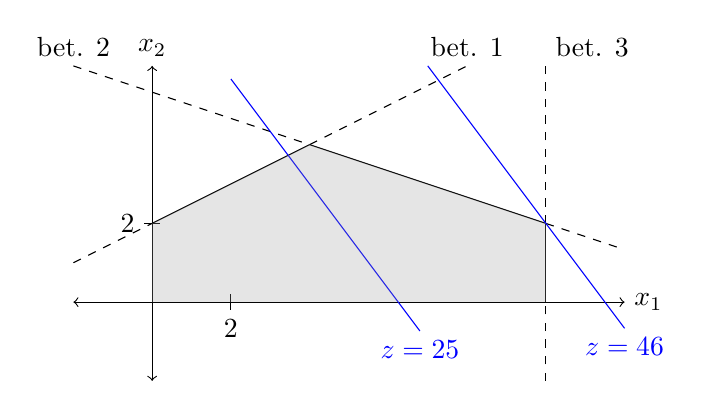
\begin{tikzpicture}
  %laver Grid. godt til når koordinater skal redigeres
  	%\draw[thin,gray!40] (-3,-1) grid (6,3); 
  %x-aksen
  	\draw[<->] (-1,0)--(6,0) node[right]{$x_1$}; 
  %y-aksen
  	\draw[<->] (0,-1)--(0,3) node[above]{$x_2$};
  	
  %akse-markeringer
  	%\node[left] (xakse) at (0,1) {2};
  	\draw[] (-0.1,1) -- (0.1,1) node[pos=0,left] {2};
  	\draw[] (1,-0.1) -- (1,0.1) node[pos=0,below] {2};
  	
  %ligning 1
	\draw[domain=-1:0,variable=\x,dashed] 	plot({\x},{0.5*\x+1});
	\draw[domain=0:2,variable=\x] 			plot({\x},{0.5*\x+1});
	\draw[domain=2:4,variable=\x,dashed] 	plot({\x},{0.5*\x+1}) node[above] {bet. 1};
	
  %ligning 2
  	\draw[domain=-1:2,variable=\x,dashed] 	plot({\x},{-(1/3)*\x+8/3}) node[above] at (-1,3) {bet. 2} ;
	\draw[domain=2:5,variable=\x] 			plot({\x},{-(1/3)*\x+8/3});
	\draw[domain=5:6,variable=\x,dashed] 	plot({\x},{-(1/3)*\x+8/3});
	

  %ligning 3
  	\draw[domain=-1:0,variable=\y,dashed] 	plot({5},{\y});
	\draw[domain=0:1,variable=\y] 			plot({5},{\y});
	\draw[domain=1:3,variable=\y,dashed] 	plot({5},{\y}) node[above right] {bet. 3};
	
  %niveaukurver
  	\draw[domain=3.5:6,variable=\x,blue] plot({\x},{-(4/3)*\x+23/3}) node[below] {$z=46$};
  	\draw[domain=1:3.4,variable=\x,blue] plot({\x},{-(4/3)*\x+25/6}) node[below] {$z=25$};
  	
  %c-vektor
  	%\draw[->,thick,red] (0,0) -- (2,1.5);

  %løsningsmængden skraveret
	\fill[gray!80,nearly transparent] (0,0) -- (0,1) -- (2,2) -- (5,1) --(5,0) --  cycle;
\end{tikzpicture}
		\captionof{figure}{Optimal løsning i den mulige mængde fundet som skæring med ligningen $z=46$.}
		\label{fig:maksprob3}
	\end{center}
	
På figuren ses det, at den største funktionsværdi $z=46$ findes i skæringen mellem bibetingelse 2 og 3.
Ved at løse bibetingelse 2 og 3 som 2 ligninger med 2 ubekendte findes det at den optimale løsning er $\vec{x}=\rvect{10 & 2}^T.$
\label{eks:maksprob3}
\end{eks}

%%%%%%%%%%%%%%%%%%%%%%%%%%%%%%%%%%%%%%%%%%%%%%%%%%%%%%%%%%%%%%%%%%%%%%%%%%%%%%%%%%%%%%
%%%%%%%%%%%%%%%%%%%%%%%%%%%%%%%%%%%%%%%%%%%%%%%%%%%%%%%%%%%%%%%%%%%%%%%%%%%%%%%%%%%%%%

\subsection{Niveaukurver}
Niveaukurver dannes ved fastsættelsen af en funktionsværdi $z=\vec{c}^T \vec{x}$. Niveaukurven er derved mængden af alle vektorer $\vec{x}$, som løser ligningen. Da målet er at maksimere $z$, er målet at finde den største $z$ for hvilken niveaukurven har en ikke-tom skæring med den mulige mængde. 

En løsningsvektor $\vec{x}$ kan omskrives til summen af en vektor parallel med $\vec{c}$, kaldet $\vec{x}_p$, og en vektor orthogonal med $\vec{c}$, kaldet $\vec{x}_o$. Her gælder det derved at, $\vec{x}_p=k\cdot \vec{c}$ for en skalar $k$, og at $\vec{x}_o^T \vec{c}=0$. Dette er muligt, da vektorrummet der er orthogonalt med $\vec{c}$ har dimension $n-1$, mens rummet dannet af $\vec{c}$ har dimension $1$. Da vil vektorrummet dannet af summen af disse rum have dimension $n$, da de to rum er orthononale. Derved kan alle løsningsvektorer $\vec{x}$ udtrykkes som summen af en vektor fra hvert af de to rum.

\begin{align*}
	f(\vec{x}) & \ = \ \vec{c}^T\vec{x}\\
	f(\vec{x_p}+\vec{x_o}) & \ = \ 
	\vec{c}^T\vec{x_p}+\vec{c}^T\vec{x_o} \ = \ 
	\vec{c}^T\vec{x_p} \ = \ 
	k\cdot \vec{c}^T\vec{c} \ = \ 
	k \cdot \Vert \vec{c} \Vert ^2
\end{align*}
Da funktionsværdien derved er lig $k \cdot \Vert \vec{c} \Vert ^2$ gælder det derved om at maksimere $k$ for maksimeringsproblemer og at minimere $k$ for minimeringsproblemer. 


Dette kan ses i Eksempel \ref{eks:maksprob3}.
\begin{comment}
Bør niveaukurve defineres????? Hvordan kan dette bruges, for at finde $z$ er egentlig bare en omskrivning, så der mangler noget argumentation for at $z$ bliver større jo længere væk fra origo man er, hvilket giver ret god mening, men er svært at argumentere for uden at starte på geometri, så måske hele dette afsnit skulle flyttes, måske skal alt om løsninger skal flyttes til geometri?
\end{comment}


\begin{eks}[Optimal løsning fundet grafisk]
Niveaukurverne $46=\vec{c}^T \vec{x}$ og $25=\vec{c}^T \vec{x}$ er på Figur \ref{fig:maksprob3} indtegnet for programmeringsprogblemet fra Eksempel \ref{eks:maksprob2}.

	\begin{center}	
		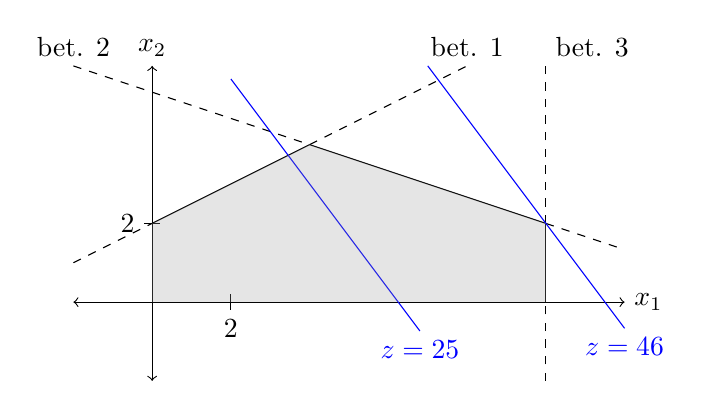
\begin{tikzpicture}
  %laver Grid. godt til når koordinater skal redigeres
  	%\draw[thin,gray!40] (-3,-1) grid (6,3); 
  %x-aksen
  	\draw[<->] (-1,0)--(6,0) node[right]{$x_1$}; 
  %y-aksen
  	\draw[<->] (0,-1)--(0,3) node[above]{$x_2$};
  	
  %akse-markeringer
  	%\node[left] (xakse) at (0,1) {2};
  	\draw[] (-0.1,1) -- (0.1,1) node[pos=0,left] {2};
  	\draw[] (1,-0.1) -- (1,0.1) node[pos=0,below] {2};
  	
  %ligning 1
	\draw[domain=-1:0,variable=\x,dashed] 	plot({\x},{0.5*\x+1});
	\draw[domain=0:2,variable=\x] 			plot({\x},{0.5*\x+1});
	\draw[domain=2:4,variable=\x,dashed] 	plot({\x},{0.5*\x+1}) node[above] {bet. 1};
	
  %ligning 2
  	\draw[domain=-1:2,variable=\x,dashed] 	plot({\x},{-(1/3)*\x+8/3}) node[above] at (-1,3) {bet. 2} ;
	\draw[domain=2:5,variable=\x] 			plot({\x},{-(1/3)*\x+8/3});
	\draw[domain=5:6,variable=\x,dashed] 	plot({\x},{-(1/3)*\x+8/3});
	

  %ligning 3
  	\draw[domain=-1:0,variable=\y,dashed] 	plot({5},{\y});
	\draw[domain=0:1,variable=\y] 			plot({5},{\y});
	\draw[domain=1:3,variable=\y,dashed] 	plot({5},{\y}) node[above right] {bet. 3};
	
  %niveaukurver
  	\draw[domain=3.5:6,variable=\x,blue] plot({\x},{-(4/3)*\x+23/3}) node[below] {$z=46$};
  	\draw[domain=1:3.4,variable=\x,blue] plot({\x},{-(4/3)*\x+25/6}) node[below] {$z=25$};
  	
  %c-vektor
  	%\draw[->,thick,red] (0,0) -- (2,1.5);

  %løsningsmængden skraveret
	\fill[gray!80,nearly transparent] (0,0) -- (0,1) -- (2,2) -- (5,1) --(5,0) --  cycle;
\end{tikzpicture}
		\captionof{figure}{Optimal løsning i den mulige mængde fundet som skæring med ligningen $z=46$.}
		\label{fig:maksprob3}
	\end{center}
	
På figuren ses det, at den største funktionsværdi $z=46$ findes i skæringen mellem bibetingelse 2 og 3.
Ved at løse bibetingelse 2 og 3 som 2 ligninger med 2 ubekendte findes det at den optimale løsning er $\vec{x}=\rvect{10 & 2}^T.$
\label{eks:maksprob3}
\end{eks}

Den anden tager udgangspunkt i resultatet fra Sætning \ref{stn:eksistens}, der siger at en \textbf{optimal løsning ?!?} altid er en basisløsning, og viser hvordan simplexer kan bruges til at vælge en basis, som vil føre til en basisløsning med optimal værdi.
Der vil derfor med udgangspunkt i %indsæt kilde
blive gennemgået definitionen for en simplex og hvordan det kan bruges til at udtrykke en basisløsning.

\section{Simplex og Basisløsninger}
Den anden løsningsmetode tager udgangspunkt i resultatet fra Sætning \ref{stn:eksistens}, der siger at en \textbf{optimal løsning ?!?} altid er en basisløsning, og viser hvordan simplexer kan bruges til at vælge en basis, som vil føre til en basisløsning med optimal værdi.
Derfor vil definitionen for en simplex, og hvordan det kan bruges til at udtrykke en basisløsning blive gennemgået i dette afsnit.
\subsection{Simplex}
For at kunne definere en simplex, er det nødvendigt først at introducere begreberne konvekskombination og konvekshyslser.
\begin{defn}[Konveks kombination]
Lad $\vec{x}^1, ...,\vec{x}^k \in \mathds{R}^n$, og $\lambda_1,..., \lambda_k \geq 0 $ være skalare, som opfylder $\sum_{i=1}^k \lambda_i =1$ da er $\sum_{i=1}^k \lambda_i \vec{x}^1$ en \textbf{konveks kombination}.
\label{def:KonveksKombination}
\end{defn}
En konveks kombination er dermed et særtilfælde af en linear kombination, hvor skalrene summer til $1$.
\begin{defn}[Konveks hylster]
Lad $\vec{x}_1, ...,\vec{x}_k \in \mathds{R}^n$, da er $C_{x} = \{\sum_{i=1}^k \lambda_i \vec{x}_i| \vec{x}_1, ...,\vec{x}_k \in \mathds{R}^n, \sum_{i=1}^k \lambda_i =1\}$ et \textbf{konveks hylster} for vektorene $\vec{x}_1, ...,\vec{x}_k$. 
\label{def:Konvekshuld}
\end{defn}
Mens, at mængden af alle konvekse kombinationer af en given mængde vektorer, kaldes et konvekshylster, og minder derfor om spandet af en mængde vektorer.
Et særtilfælde af konveksehylstre er en simplex.
\begin{defn}[Simplex]
Lad $C_x$ være et konveks huld, af $k+1$ affint lineært uafhængige vektorer, da er $C_x$ en $k$-dimentionel \textbf{Simplex}.
\label{def:simplex}
\end{defn}
%Eftersom det konveksehylster, kun består af konvekse kombinationer, vil det give mening at det udgør en konveks mængde.
%\begin{stn}
%Konveks huldet $C_x = \{\sum_{i=1}^k \lambda_i \vec{x}_1| \vec{x}_1, ...,\vec{x}_k \in \mathds{R}^n, \sum_{i=1}^k \lambda_i =1\}$ over en endelig mængde vektorer, er en konveks mængde
%\end{stn}
%\begin{proof}
%Lad $\vec{z}, \vec{y}\in C_x = \{\sum_{i=1}^k \lambda_i \vec{x}_i| \vec{x}_1, ...,\vec{x}_k \in \mathds{R}^n, \sum_{i=1}^k \lambda_i =1\}$ være vilkårlige vektorer da må $\vec{z}= \sum_{i=1}^k \gamma_i \vec{x}_i, \vec{y}= \sum_{i=1}^k \eta_i \vec{x}_i$ for $\sum_{i=1}^k \gamma_i = 1$ og  $\sum_{i=1}^k \eta_i = 1$. 
%Derfor må
%\begin{align*}
%	\lambda \vec{z} + (1- \lambda) \vec{y} &= \lambda\sum_{i=1}^k \gamma_i \vec{x}_i + (1-\lambda)\sum_{i=1}^k \eta_i \vec{x}_i
%	\\ &=\sum_{i=1}^k (\lambda \gamma_i+(1-\lambda)\eta_i )\vec{x}_i,
%\end{align*}
%For $\lambda \in [0,1]$.
%Betragt nu konstanterne 
%\begin{align*}
%	\sum_{i=1}^k (\lambda \gamma_i+(1-\lambda)\eta_i ) &= \lambda \sum_{i=1}^k \gamma_i + (1 - \lambda) \sum_{i=1}^k \eta_i 
%	\\ &= \lambda \cdot 1 + (1 - \lambda) \cdot 1 = 1
%\end{align*}
%Hvorfor at $\lambda \vec{z} + (1- \lambda) \vec{y} $ er en konveks kombination af vektorene $\vec{x}_1, ...,\vec{x}_k $, ifølge Definition \ref{def:KonveksKombination}. 
%Derfor må $ \lambda \vec{z} + (1- \lambda) \vec{y} \in C_x$, hvorfor at $C_x$ er konveks ifølge Definition \ref{def:Konveks}.
%Og sætningen er bevist.
%\end{proof}
%Dermed er en simplex en konveks mængde udspændt af affint lineære vektorer.
%Dette kan bruges til geometrisk at repræsenterer basisløsninger og deres basis matrix.
Simplexer kan da bruges til at repræcenterer en basisløsning.

\subsection{Simplex og Basisløsninger}
For at en basisløsning kan blive repræsenteret af en simplex, kræver det, at basisløsningen er en løsning til et lineært programmerings problem på konveks form.
\begin{defn}[Konveks form]
Et lineært programmeringsproblem på formen:
\begin{center}
\begin{tabular}{l	>{$}l<{$}}
Minimer			& \vec{c}^T\vec{x} \\
med hensyn til 	& A\vec{x} = \vec{b}\\
og				& \vec{e}^T\vec{x} = 1\\
og 				& \vec{x} \geq \vec{0}, 
\end{tabular}
\end{center}
for $\vec{e} =\rvect{1 & \cdots & 1 }^T$,  siges at være på \textbf{konveks form}, og bibetingelsen $\vec{e}^T\vec{x} = 1$ kaldes \textbf{konveksbibetingelsen}.
\end{defn}
Grunden til at $\vec{e}^T\vec{x}=1$ kaldes konveksbibetingelsen, er fordi den sørger for at $\vec{b}$ er en konvekskombination af søjlerne i matricen $A$.
\begin{stn}[Konveks form]
Et hvert lineært programmeringsproblem med $ \vec{0} \notin P$ kan omskrives til konveks form.
\end{stn}
\begin{proof}
I Kapitel \ref{Afsnit:LinProg}
er det gennemgået hvordan alle lineært programmerings problemer kan skrives på standard form med ligheder, derfor er det kun nødvendigt at vise at et hvert lineært programmerings problem på standard form med ligheder kan omskrives til konveks form.
\\ Lad derfor $\vec{x} \neq \vec{0}$ være en løsning til et lineært programmerings problem på standard form med ligheder, da vil 
\begin{align*}
\vec{e}^T \vec{x} = \lambda,
\end{align*}
hvor $\lambda$ er en positiv skalar.
Da vil 
\begin{align*}
\vec{e}^T\vec{x}' = \vec{e}^T\frac{1}{\lambda}\vec{x} = 1.
\end{align*}
For at sørge for at den konvekse form har samme løsningsmængde som det lineære programmerings problem på standard form med ligheder, multipliceres $A$ med $\lambda$, hvorefter at
\begin{align*}
A' \vec{x}' = \lambda A \frac{1}{\lambda} \vec{x} = A \vec{x} = \vec{b}.
\end{align*}
Derfor må et hvert lineært programmeringsproblem med $\vec{b}\neq \vec{0}$ kan omskrives til konveks form.
\end{proof}
Så længe at nulvektoren ikke er en løsning kan ethvert lineært programmerings problem derfor omskrives til konveks form.
Grunden til, nulvektoren ikke må være en løsning er, at prikproduktet af en vilkårlig vektor og nulvektoren vil altid give nul, hvorfor konveksbibetingelsen ikke kan overholdes.
Dermed vil en basisløsning til stort set hvilket som helst lineært programmerings problem, kunne repræsenteres ved en simplex.
\begin{stn}
Lad $\vec{x}$ være en basisløsning til et lineært problem på konveks form, med basismatrix $B$, da vil
\begin{align*}
S_x = \{\vec{v} \in \mathds{R}^{m+2} \mid \vec{v} = \sum_{i=1}^{m+1} \lambda_i \rvect{\vec{B}_i & c_i}^T, \sum_{i=1}^{m+1} \lambda = 1\}
\end{align*}
være en simplex, og $\vec{b}_x = \rvect{\vec{b}& z_x}^T \in S_x$.
\end{stn}
Bemærk at da problemet er på konveks form vil $|I_B| = m+1$ hvis $A$ er en $n\times m$ matrix, da det i følge Sætning \ref{stn:PQ}
kan antages at alle rækker er lineært uafhængige med $\vec{e}$.
\begin{proof}
For at $\rvect{\vec{A}_i & c_i}^T$ for $i \in I_B$ udspænder en simplex, skal vektorene være affint lineært uafhængige.
Derfor vises først at $\rvect{\vec{A}_i & c_i}^T$ for $i \in I_B$ er affint lineært uafhængige.
Antag for modstrid, at de ikke er, da vil der eksistere skalare forskelligt fra $0$ så
\begin{align*}
\sum_{i = 1}^{m} \lambda_i (\vec{A}_{B(i)} - \vec{A}_{B(m+1)} =  \vec{0} \qquad \wedge \qquad \sum_{i=1}^{m} \lambda_i (c_i - c_{m+1})= 0.
\end{align*}
Betragt nu kun $\sum_{i = 1}^{m} \lambda_i (\vec{A}_{B(i)} - \vec{A}_{B(m+1)} =  \vec{0}$, det medføre, at
\begin{align*}
\sum_{i = 1}^{m} \lambda'_i \vec{A}_{B(i)} = \vec{A}_{B(m+1)},
\end{align*}
hvor $\lambda'_i = \lambda_i/(\sum_{i=1}^m \lambda_i)$.
Derfor følger det, hvis de ikke er affint lineært uafhængige, så er $\vec{A}_{B(m+1)}$ en linear kombination af $\vec{A}_{B(i)}$ for $i  \in i,..., m$.
Det strider mod, at $\vec{x}$ er en basisløsning, og søjlerne $\vec{A}_i$ svare til basis variablene for $i \in I_B$, derfor må vektorerne være affint lineært uafhængige. 
Dermed udgør alle konveksekombinationer af $B_i$ for $i \in I_B$ en simplex, $S_x$.
\\ Så vises det, at $\vec{b} \in S_x$. 
Det følger af Definition \ref{def:simplex},
at $\vec{b}_x\in S_x$, hvis der eksistere skalare, der opfylder $\sum_{i=1}^{m+1} \lambda_i = 1$, så $\sum_{i=1}^{m+1}\lambda_i B_{B(i)}  = \vec{b}_x$.
Da $\vec{x}$ er en basisløsning, følger det, at $B \vec{x}_B = \vec{b}_x$ og da $\vec{x}$ er betinget af konveksbetingelsen og $x_i = 0 $ for $i \notin I_B$, må $\sum_{i=1}^{m+1} x_{B(i)} = 1$, hvorfor det følger, at $\vec{b}_x \in S_x$.
\end{proof}
Bemærk at beviset kun inddirekte beviser at søjlerne i en basismarix udspænder en simplex, det kan konkluderes da $B_i$ kun er affint lineær uafhængige fordi $A_{B(i)}$ er, derfor må de også udspænde en simplex, hvor $\vec{b}$ er et element.
\begin{defn}[Simplex forbundet med basisløsning]
Lad $\vec{x}$ være en basisløsning så $x_i = 0$ hvis $i \notin I_B$, da er $S_x$ \textbf{simplexen forbundet med basisløsning $\vec{x}$}, hvis simplexen er lig konvekshuldet udspændt af søjlerne af $\rvect{\vec{A}_i & c_i}^T$ for $i \in I_B$.
\end{defn}
Grunden til at vektorene udvides, er illustreret på Figur \ref{fig:simplex}. 
\begin{center}
	\begin{tikzpicture}
  %x-aksen
  	\draw[->] (-1,0)--(6,0) node[right]{$x$}; 
  %y-aksen
  	\draw[->] (0,-1)--(0,4.2) node[above]{$z$};
  	
  	
%Punkter
    \node[] (A) at (0.5,0.3) {$A$};
    \node[] (B) at (5, 3.5) {$B$};
    \node[] (C) at (3.5, 4) {$C$};
    \node[] (D) at (1, 2) {$D$};
    \node[] (b) at ( 2.5, 0) {$b$};
    
%Simplexer
    \path[thick, color=blue] (A) edge (B);
    \path[thick, color=blue] (D) edge (B);
    \path[thick, color=blue] (D) edge (C);

% Z
 	\draw[domain=0:4,variable=\y, thick, color = orange] 	plot({2.5},{\y});   
  	
\end{tikzpicture}
	\captionof{figure}{ 
	%Hvis de udvidet vektorer antages at være punkter; $A$, $B$, $C$, $D$, da vil koordinaterne svarende til indgangende i søjlerne i basismatrixen ligger i samme $m+1$ dimentionelle rum, mens at punkterne svarende til koefficienterne i objektfunktionen ligge i den $m+2$ dimension. Derfor vil objektfunktions værdi, anses som $\rvect{ \vec{b} & z }^T$, den orange linje, anses som skæringen mellem simplexerne, de blå linjer. 
	}
	\label{fig:simplex}
\end{center}
Det kan bruges til at finde den optimale basisløsning. 
%Grunden til at vektorene udvides, er fordi de udvidet vektorer, antages at være punkter i stedet, da vil koordinaterne svarende til indgangende i søjlerne i basismatrixen ligger i samme $m+1$ dimentionelle rum, mens at punkterne svarende til koefficienterne i objektfunktionen ligge i den $m+2$ dimension.  
%Derfor vil ændringen i værdien for objektfunktionen for to basisløsninger kunne ses som afstanden mellem de to simplexer forbundet med basisløsningerne i den $m+2$ dimension.
\begin{prop}
Afstanden mellem to simplex $S_x$ og $S_y$ forbundet med basisløsningerne $\vec{x}$ og $\vec{y}$ er $|z_x - z_y|$.
\end{prop}
\begin{proof}
For at vise proportionen findes længden af $\rvect{B_x & \vec{c}_B}^T \vec{x} - \rvect{B_y & \vec{c}_y}^T \vec{y}$
\begin{align*}
 \Vert \rvect{B_x & \vec{c}_B}^T \vec{x} - \rvect{B_y & \vec{c}_y}^T \vec{y} \Vert & =  \Vert \rvect{\vec{b} & z_x}^T  - \rvect{\vec{b} & z_y}^T  \Vert
 \\ & = \Vert \rvect{0 & z_x - z_y}^T \Vert = |z_x - z_y|.
\end{align*}
Dermed kan det konkluderes, at afstanden mellem to simplex $S_x$ og $S_y$ forbundet med basisløsningerne $\vec{x}$ og $\vec{y}$ er $|z_x - z_y|$.
\end{proof}
Det betyder, hvis objektfunktionen skal minimeres, skal simplexen, der ligger tættes på $z = 0$, findes, hvorfor der altid skal vælges en simplex, der ligger lavere end den forrige, dvs. en simpelex, hvor en ny basisvariable har en lavere koefficient $c_i$ end den gamle basisværdi.
Det er det simplexmetoden tager udgangspunkt i.




\chapter{Simplex Metoden}
Af forrige kapitel fremgik det, at den optimale løsning altid vil være en mulig basisløsning, og af Sætning \ref{stn:kravtilbasis}
fremgår det, hvordan en basisløsning findes. 
Problemet er, at hvis alle basisløsninger skal testes for et standard problem med uligheder, skal optil $\binom{n}{m}$ muligheder testes. 
Derfor er det nødvendigt, at finde en metode, hvorpå den optimale løsning kan findes uden at skulle kigge på hvert enkelt tilfælde. 
En af metoderne, som kan anvendes, er Simplex metoden. I dette kapitel vil Simplex metoden, og forskellige implementeringer af metoden, derfor blive gennemgået med udgangspunkt i .

\section{Udledning af Simplex metoden}
Simplex metoden starter med en basisløsning, og går så i en mulig retning, indtil den finder en ny basisløsning.

\begin{defn}[Mulig retning]
Lad $\vec{x} \in P$. En vektor $\vec{d}$ er en \textbf{mulig retning} fra $\vec{x}$, hvis der eksisterer en skalar $\theta > 0$, således at $\vec{x}+\theta\vec{d} \in P$ 
\end{defn}

Derfor skal den mulige retning introducere en ny basisvariabel til løsningen.

\begin{lma}[Den $j$'te retningsvektor]
Lad $\vec{x} \in P$ være en basisløsning med basis matrix $B$, og lad $\vec{d}_j  \in \mathds{R}^n$ være en mulig retningsvektor, så $\vec{x}' = \vec{x}+ \theta\vec{d}_j$ introducerer basisvariablen $x_j'$ og kun $x_j'$ til løsningen, for en skalar $\theta$.
Da vil $\vec{d}_j$ være givet; så $\vec{d}_{j,B} = -B^{-1}\vec{A}_j$, $d_{j,j} = 1$ og $d_{i,j} = 0$ for $i \neq j$ og $ i,j \notin I_B$.
\label{lma:retningsvektor}
\end{lma}

\begin{proof}
Hvis $\vec{x}'$ skal introducere $x_j'$ til løsningen skal $x_j + \theta d_{j,j} > 0$. 
Da $x_j = 0$ ifølge antagelsen om, at $\vec{x}$ er en basisløsning, og $\theta$ er en skalar, kan $d_j$ sættes lig $1$ uden at miste generalitet. 
På samme måde må $d_i = 0$ for $i \neq j$ og $i \notin I_B$, da $x_i' = 0$, for ikke at introducere $x_i'$ til løsningen.
Da $\vec{d}$ er en mulig retningsvektor, vil $\vec{x}' \in P$, hvormed at $A\vec{x}' = A\vec{x}+ \theta A\vec{d}_j = \vec{b}$. 
Fordi $A\vec{x} = \vec{b}$, medfører det, at $A\vec{d}_j = \vec{0}$.
Det følger derfor, at
\begin{align*}
A\vec{d}_j = B \vec{d}_B + \sum_{i \notin I_B} \vec{A}_id_i = B\vec{d}_B + \vec{A}_j = \vec{0} \Rightarrow
\\ \vec{d}_j = -B^{-1}\vec{A_J}.
\end{align*}
Bemærk at $B^{-1}$ eksisterer ifølge Sætning. 
Lemmaet er hermed bevist.
\end{proof}

Den nye vektor $\vec{x}'$ må kun have $m$ basisvariable for at være en basisløsning, og da $\vec{d}_j$ introducerer en ny variabel til løsningen, skal $\theta^*\vec{d}$ også fjerne en variabel fra  løsningen.

\begin{lma}[Den $j$te skalar]
Lad $\vec{x} \in P$ være en basisløsning med basis matrix $B$, og lad $\vec{d}_j$ være den $j$'te retningsvektor, så $I_d = \{i \mid d_i < 0, \, i  \in I_B\}$, og $\theta^* = \min_{i \in I_d}\{\frac{x_i}{|d_i|}\}=\frac{x_l}{|d_l|} > 0$ . 
Så vil $\vec{x}' = \vec{x}+ \theta^* \vec{d}_j \in P$ fjerne $x_l'$ fra løsningen, hvis $P$ ikke indeholder en positiv halvlinje.
\label{lma:skalar}
\end{lma}

\begin{bem}
Da $\vec{d}_j$ er en mulig retningsvektor, er $x_i\neq 0$ for $i \in I_d$, hvorfor $\theta^* > 0$.
\end{bem}

\begin{proof}
Antag først, at $I_d = \emptyset$, da vil $x_i' \geq 0 \ \forall \ \theta \geq 0$. 
Hvormed, at $\vec{x}' \in P \ \forall \ \theta \geq 0$, og $P$ vil derfor indeholde en positiv halvlinje, hvormed det kan konkluderes, at $P$ ikke er tom, og $\theta^*$ eksisterer.
Derfor må $x_l' = x_l + \theta^* d_l = x_l + \frac{x_l}{|d_l|}d_l = x_l - x_l = 0$ dermed fjerne $\vec{x}'$ $x_l$ fra løsningen.
Til sidst vises, at $\vec{x}' \in P$. Betragt derfor $x_i' = x_i + \theta^* d_i$ for $i \neq l$, $i \in I_d$ da vil
\begin{align*}
x_i' = x_i + \theta^* d_i = x_i + \frac{x_l}{|d_l|}d_i \geq x_i + \frac{x_i}{|d_i|}d_i = 0,
\end{align*}
da $d_i < 0$ og $\frac{x_l}{|d_l|} \leq \frac{x_i}{|d_i|}$, hvorfor alle indgange forbliver ikke-negative, og $\vec{x}'$ er dermed en mulig løsning.
\end{proof}

\begin{bem}
Lad $x'_j = \theta^* >  0$, da $d_j = 1$ og $\theta^* > 0$. Da fjerner $\vec{x}'$ ikke $x_j'$ fra løsningen.
\end{bem}

Dermed kan $\vec{x}'$ at have $m$ basisvariable under antagelsen om, at $\vec{x}'$ ikke er degenerativ. Er $\vec{x}'$ degererate, ville der ikke være et entydigt indeks $l$ som opfyldte at $min_{i \in I_d}\{\frac{x_i}{|d_i|}\}=\frac{x_l}{|d_l|}$, hvormed at flere af basisvariablene vil blive $0$. 

\begin{stn}
Lad $\vec{x}\in P$ være en mulig basisløsning, med basismatrix $B$, da vil $\vec{x}' = \vec{x}+ \theta^*\vec{d}_j$ også være en mulig basisløsning, hvis $P$ ikke indeholder en positiv halvlinje.
\end{stn}

\begin{proof}
For at vise, at $\vec{x}'$ er en basisløsning, bemærkes at $x_i = 0$ for $i \notin I_{B'} = I_B\setminus\{l\}\cup\{j\}$ samt, at basismatricen for $\vec{x}'$ er matricen $B'$ med søjlerne $\vec{A}_i$ for $i \in I_{B'}$. 
Det følger derfor af Sætning \ref{stn:kravtilbasis},
at $\vec{x}'$ er en basisløsning, hvis søjlerne i $B'$ er lineært uafhængige.
Antag derfor for modstrid, at søjlerne er lineært afhængige, da følger det af Definition \ref{defn_lin_uafh},
at
\begin{align*}
 \sum_{i \in I_{B'}} \lambda_i \vec{A}_i = \vec{0}.
\end{align*}
Da $B$ og $B'$ kun er forskellige i en søjle, må
\begin{align*}
 \\ \sum_{i \in I_{B'}}  B^{-1} \lambda_i \vec{A}_i  =\sum_{i \in I_{B'}\setminus \{j\}} \vec{e_i} + B^{-1} \lambda_j \vec{A}_j = \vec{0}.
\end{align*}

Det vil sige, at søjlerne i $B'$ er lineært uafhængige, hvis $A_{jl} = 0$.
Bemærk, at $B^{-1} \lambda_j A_j = - \vec{d}_B$, hvis $l$'te indgang pr. definition er skarpt mindre end $0$, og $A_{jl} \neq 0$.
Alle søjler i $B'$ er altså lineært uafhængige, hvorfor alle rækker er lineært uafhængige, og $\vec{x}'$ er en basisløsning.
Bemærk, at da $\vec{x}\in P$ og $P$ ikke indeholder en positiv halvlinje, vil $\vec{x}' \in P$ ifølge Lemma \ref{lma:skalar}, hvormed $\vec{x}'$ er en mulig basisløsning.
\end{proof}

Det er nu vist, hvordan det er muligt at gå fra én basisløsning til en anden.
Bemærk, at de to løsninger er naboløsninger, da det er antaget, at ingen af dem er degenerative, og der derfor kun bliver introduceret én ny variabel og fjernet en gammel, hvorfor løsningerne må dele samme krav pånær ét. 
Det er nu nødvendigt at finde en måde, så den basisløsning, der findes, minimerer objektfunktionen mere end den foregående. Ellers vil alle basisløsninger stadig skulle tjekkes. 

\begin{stn}[Ændring i omkostning]
Lad $\vec{x}$ være en basisløsning, med basismatrix $B$, da er ændringen i objektfunktionen, ved at introducere $x_j$ til løsningen, givet ved
\begin{align*}
 \Delta c_j = c_j-\vec{c}_B B^{-1}\vec{A_j}.
\end{align*}
\label{stn:Deltac}
\end{stn}

\begin{proof}
Antag først, at $x_j$ ikke er en basisvariabel til at starte med, da vil den $j$'te retningsvektor introducere $x_j$ til løsningen, hvorfor,
\begin{align*}
\Delta c_j = \vec{c}^T(\vec{x}+ \vec{d}) - \vec{c}^T\vec{x} = \vec{c}^T\vec{d} = \sum_{i \in I_B} c_i d_i + c_j.
\end{align*}
Lad nu $\vec{c}_B = \rvect{c_{B(1)}& \cdots & c_{B(m)}}$, da vil
\begin{align}
\Delta c_j =\vec{c}_B\vec{d}_B+ c_j = c_j-\vec{c}_B B^{-1}\vec{A_j}.
\end{align}
Antag nu, at $x_j$ er en basisvariabel, da vil 
\begin{align*}
\Delta c_j = \vec{c}^T\vec{x}- \vec{c}^T\vec{x} = 0.
\end{align*}
Det undersøges derfor, om $ c_j-\vec{c}_B B^{-1}\vec{A_j}= 0$, hvis $x_j$ er en basisvariable.
\begin{align*}
 \Delta c_j = c_j-\vec{c}_B^T B^{-1}\vec{A_j} = c_j - \vec{c}_B^T \vec{e_j} = c_j - c_j = 0.
\end{align*}
Det kan derfor konkluderes, at $\Delta c_j = c_j-\vec{c}_B B^{-1}\vec{A_j}$ for ethvert $x$.
\end{proof}

Det må derfor være bedst at gå enten i den retning, hvor $\Delta c_j$ er størst, eller hvor $\theta^*\Delta c_j$ er størst. 
Hvis der ikke sker en ændring, eller ændringen forstørrer objektfunktionen, må den fundne basisløsning nødvendigvis være optimal.

\begin{stn}[Optimal omkostning]
Lad $\vec{x}$ være en basisløsning med basismatrix $B$, så er $\vec{x}$ optimal, hvis og kun hvis $\Delta c_j \geq 0$ for alle $j$.
\label{stn:optimalDeltaC}
\end{stn}.

\begin{proof}
Antag først, at $\vec{x}$ er optimal, da vil $\vec{c}^T\vec{x} \leq \vec{c}^T\vec{y}$ for alle $\vec{y} \in P$. 
Antag for modstrid, at $\Delta c_j < 0$ for en basisvariabel $x_j$, da følger det, at $\vec{c}^T(\vec{x}+\theta^*\vec{d}) = \vec{c}^T\vec{x} + \Delta c_j \leq \vec{c}^T\vec{x}$, hvilket strider mod antagelsen om, at $\vec{x}$ er optimal.
Antag nu, at $\Delta c_j \geq 0$, og lad $\vec{y}$ være en vilkårlig vektor i $P$, samt lad $\vec{d}=\vec{x}'-\vec{x}$.
Bemærk, at $A\vec{d} = A\vec{x}'- A\vec{x} =  \vec{b} - \vec{b} =\vec{0}$.
Lad nu $\vec{d}_B = \rvect{d_{B(1)} & \cdots & d_{B(m)}}^T$, og lad $N= \{i \leq n| i \neq B(1),...,B(m)\}$, da kan matrix-vektorproduktet omskrives til:
\begin{align*}
	B\vec{d}_B + \sum_{i \in N} \vec{A}_i d_i = \vec{0} \qquad \Rightarrow
	\\ \vec{d}_B = - B^{-1}\sum_{i \in N} \vec{A}_i d_i
\end{align*}
Bemærk, at det benyttes, at $B$ er invertibel ifølge Sætning. %Mangler
Da tages objektfunktionen til $\vec{d}$ for at finde omkostningen, af at gå fra $\vec{x}$ til $\vec{x}'$.
\begin{align*}
 \vec{c}^T\vec{d} &= \vec{c}_B^T\vec{d}_B + \sum_{i \in N} c_i d_i 
 \\&= \vec{c}_B^T(- B^{-1}\sum_{i \in N} \vec{A}_i d_i) + \sum_{i \in N} c_i d_i  
 \\&= \sum_{i \in N} (- \vec{c}_B^T B^{-1} \vec{A}_i d_i) +  c_i d_i 
 \\&= \sum_{i \in N} ( c_i - \vec{c}_B^TB^{-1}\vec{A}_i ) d_i
\end{align*}
Det følger af Sætning \ref{stn:Deltac} at $\Delta c_i = c_i - \vec{c}_B^TB^{-1}\vec{A}_i $, hvorfor
\begin{align*}
\vec{c}^T\vec{d} = \sum_{i \in N} \Delta c_i d_i.
\end{align*}
Da $\vec{x}$ er en basisløsning må $x_i = 0$ for $i \in N$, og da $\vec{x}' \in P$ må $\vec{x}' \geq \vec{0}$. Dermed må $d_i = x_i' - x_i \geq 0$. Da $\Delta c_i$ var antaget at være ikke-negativ, medfører det at
\begin{align*}
\vec{c}^T\vec{d} = \vec{c}^T\vec{y}-\vec{c}^T\vec{x} \geq 0 \qquad \Rightarrow
\\ \vec{c}^T\vec{x} \leq \vec{c}^T\vec{x}'
\end{align*}
for ethvert $\vec{x}' \in P$. Da $\vec{x}'$ var vilkårligt valgt, må $\vec{x}$ være optimal.
\end{proof}

Det kan alt sammen opsummeres til Simplex metoden.

\begin{pro}[label=pro:simplex,style=ingental]{Procedure for Simplex metoden}
1. Vælg en basisløsning $\vec{x}$ med basismatrix $B$
2. Beregn $\Delta c_j$ for alle $j \notin I_B$. 
   Hvis $\Delta c_j\geq 0$ for alle $j \notin I_B$ 
   	   stop, $\vec{x}$ er optimal.
   Hvis $\Delta c_j < 0$ for en $j \notin I_B$
       vælg mindste $c_j$.
3. Find $\vec{d}_j$
   Hvis $d_i \geq 0 $ for alle $i \in I_B$ 
       stop, den optimaleværdi er $- \infty$.
   Hvis $d_i < 0 $ for mindst et $i \in I_B$ 
       vælg $B(l)$ så $\frac{x_{B(l)}}{d_{B(l)}}\leq \frac{x_i}{d_i} $ for ethvert $i \in I_B$
4. Find $\theta^*$
5. Find den nye basisvektor og basismatrix.
6. Gå til step 2.
\end{pro}

Til sidst vises, at Simplex metoden altid vil finde frem til den optimale løsning efter et endeligt antal iterationer.

\begin{stn}
Lad $P \neq \emptyset$, da stopper Simplex metoden efter et endeligt antal iterationer, enten ved at finde den optimale løsning eller at den optimale værdi er $- \infty$.
\end{stn}

\begin{proof}
Antag først, at Simplex metoden stopper efter step $2$ i Program \ref{pro:simplex}, da følger det af Sætning \ref{stn:optimalDeltaC}
at basisløsningen er optimal, og Simplex metoden har derfor fundet den optimale løsning.\\ 
Antag nu, at Simplex metoden stopper efter step $3$ i Program \ref{pro:simplex}, da følger det af beviset for Lemma \ref{lma:skalar}, at $P$ indeholder en linje, hvorfor det følger af Afsnit \ref{sec:eksistens},
at den optimale værdi er $-\infty$.\\ 
Da der kun er en endelig mængde basisløsninger ifølge Korollar \ref{kor:endeligbasis} må Simplex metoden altid stoppe, medmindre den cirkulere igennem de samme basisløsninger.
Da den $j$'te retningsvektor altid vælges så $\Delta c_j < 0$, må den samme basisløsning aldrig kunne blive besøgt mere end én gang, hvorfor der ikke kan opstå en ring, og Simplex metoden må derfor stoppe efter et endeligt antal iterationer.
\end{proof} 

\section{Implementering af Simplex Metoden}

Der findes forskellige måder at implementere Simplex metoden, det kan blandt gøres ved brug af Fuld tabel og Store-M metoden. Desuden kan den leksikografiske pivotregel forhindre, at Simplex metoden har et undeligt antal iterationer. 

\subsection{Fuld tabel}
Fuld tabel metoden er en metode til implementering af Simplex. Et standard minimeringsproblem $\vec{c}^T\vec{x}$, med bibetingelserne $A\vec{x} \geq \vec{b}$, kan ved brug af slack-variable omskrives til $A\vec{x}+\vec{s}=\vec{b}$. Givet en aktuel basis, $B$, kan ligheden også udtrykkes som  $B^{-1}\vec{b}=B^{-1}A\vec{x}$. Fuld tabel metoden bruger $m \times (n+1)$ matricen $B^{-1}[\vec{b} \ \mid \ A]$.\\

\begin{defn}[Simplex tabel]
Lad $z=\vec{c}^T\vec{x}$ være en objektfunktion med lineært uafhængige bibetingelser for et minimeringsproblem $A\vec{x} \geq \vec{b}$, så er en \textbf{Simplex tabel},\\
\begin{center}
\begin{tabular}{| c | c |}
  \hline
  $-\vec{c_B}\vec{x}_B$&$\Delta\vec{c}$ \\ \hline			
  $B^{-1}\vec{b}$ & $B^{-1}A$ \\ \hline
\end{tabular}
\end{center}
hvor $-\vec{c_B}\vec{x}_B$ er det negative af den aktuelle omkostning. 
\end{defn}


På mere udvidet form vil Simplex tabellen se således ud,
\begin{center}
\begin{tabular}{| r|r r r|}
  \hline	
  $-\vec{c_B}\vec{x}_B$&$\Delta c_1 $ & $\dots$ &$\Delta c_n$\\ \hline	
  $x_{B(1)}$ &	| & & |\\	
  $\vdots$  & $B^{-1}\vec{A}_1$ & $\hdots$ & $B^{-1}\vec{A}_n$\\
   $x_{B(m)}$ &	| & & |\\
   \hline
\end{tabular}
\end{center}
Søjlen $B^{-1}\vec{b}$ kaldes den nulte søjle, mens den øverste række kaldes den nulte række.

\begin{pro} [label=pro:simplex,numbers=none,xleftmargin=0em] {Fuld tabel metoden}
1. Start med en tabel til basismatricen $B$ og den tilhørende mulige basisløsning $\vec{x}$.
2. Undersøg den reducerede omkostning i den nulte række. Hvis de alle er ikke-negative, er den aktuelle løsning optimal. Elles vælges et $j$, hvor $\Delta c_j <0$.
3. Betragt vektoren $\vec{u}=B^{-1}\vec{A}_j$, som er den $j$'te søjle i tabellen. Hvis alle komponenterne i $\vec{u}$ er $\quad$ negative, er den optimale omkostning $-\infty$.
4. For hvert $i$, hvor $u_i$ er positiv, beregn forholdet $\frac{x_{B(i)}}{u_i}$. Lad $l$ være indeks for rækken, hvor forholdet er mindst. Søjlen $\vec{A}_{B(l)}$ forlader basen, og $\vec{A}_j$ indtræder i basen. 
5. Læg et multiplum af den $l$'te række til alle rækker, således at $u_l$ bliver $1$ og alle andre indgange i pivot søjlen bliver $0$
6. Gentag proceduren fra trin $2$. 
\end{pro}
For at starte Simplex metoden skal der bruges en mulig basisløsning. Hvis problemet er på formen $A\vec{x} \leq \vec{b}$, og $\vec{b} \geq \vec{0}$, vil der altid kunne findes en mulig basisløsning. Denne findes ved at omskrive problemet ved hjælp af slack-variable $A\vec{x} +\vec{s}= \vec{b}$. Vektoren givet ved $[\vec{x},\vec{s}]^T$, hvor $\vec{x}=\vec{0}$ og $\vec{s}=\vec{b}$, er en mulig basisløsning. 
\begin{eks}[Fuld Tabel Metoden]
Betragt det lineære progammeringsproblem
\begin{center}
\begin{tabular}{ l c c  c  r }
Minimer &$-10x_1$&$-12x_2$ & $-12x_3$&\\
I forhold til: &$x_1$&+$2x_2 $&+$2x_3$ & $\leq 20$\\
&$2x_1$& $+x_2$& $+2x_3$ & $\leq 20$\\
&$2x_1$&$+2x_2$&$+x_3$&$\leq 20$\\
$x_1,x_2,x_3\geq 0$.
\end{tabular}
\end{center}

Nu indførers slack-variable, så ulighederne bliver til ligheder. 
\begin{center}
\begin{tabular}{ l c c  c c c c r }
Minimer &$-10x_1$&$-12x_2$ & $-12x_3$&&&\\
I forhold til: &$x_1$&+$2x_2 $&+$2x_3$ &$+x_4$&& &$=20$\\
&$2x_1$& $+x_2$& $+2x_3$ & & $+x_5$ &&$=20$\\
&$2x_1$&$+2x_2$&$+x_3$&&&$+x_6$&$=20$\\
$x_1,x_2,x_3,x_4,x_5,x_6\geq 0$
\end{tabular}
\end{center}

Trin 1\\
Nu er $\vec{x}^T=[0,0,0,20,20,20]$ en mulig basisløsning, hvor $B(1)=4,B(2)=5$ og $B(3)=6$. Den tilhørende basismatrix er identitesmatricen, $I_3$. 
\begin{center}
\begin{tabular}{|r| r|r r r r r r|}
  \hline	
  &$0$&$-10$ &$-10$&$-10$&$0$&$0$&$0$\\ \hline	
  $x_4=$&$20$&$1$&$2$&$2$&$1$&$0$&$0$\\	
  $x_5=$&$20$&$2$&$1$&$2$&$0$&$1$&$0$\\
  $x_6=$&$20$&$2$&$2$&$1$&$0$&$0$&$1$\\
   \hline
\end{tabular}
\end{center}

Trin 2\\
I den nulte række findes $3$ negative værdier. Den reducerede omkostning for $x_1$ er negativ. Den indtræder derfor i basen. \\
\\
Trin 3\\
$\vec{u}^T=[1,2,2]$. Det ses, at alle komponenterne er positive. \\
\\
Trin 4\\
For at bestemme hvilken række, der skal være pivotrække udregnes forholdet $\frac{x_{B(i)}}{u_i}$. 
\begin{align*}
\frac{x_{B(1)}}{u_1}=\frac{20}{1}=20\\
\frac{x_{B(2)}}{u_2}=\frac{20}{2}=10\\
\frac{x_{B(3)}}{u_3}=\frac{20}{2}=10\\
\end{align*}
Det ses, at forholdet for $i=2$ og $i=3$ er det samme. Da vælges $l$ til at være række $2$. \\
\\
Trin 5\\
Den nye tabel er givet ved:
\begin{center}
\begin{tabular}{|r| r|r r r r r r|}
  \hline	
  &$100$&$0$ &$-7$&$-2$&$0$&$5$&$0$\\ \hline	
  $x_4=$&$10$&$0$&$1.5$&$1$&$1$&$-0.5$&$0$\\	
  $x_1=$&$10$&$1$&$0.5$&$1$&$0$&$0.5$&$0$\\
  $x_6=$&$0$&$0$&$1$&$-1$&$0$&$-1$&$1$\\
   \hline
\end{tabular}
\end{center}
I denne tabel er den reducerede omkostning for $x_2$ og $x_3$ negativ. Derfor gennemgås procedureren igen fra Trin 2.\\
$x_3$ vælges til at indtræde i basen. Efter procedureren er gennemgået er tabellen givet ved. 
\begin{center}
\begin{tabular}{|r| r|r r r r r r|}
  \hline	
  &$120$&$0$ &$-4$&$0$&$2$&$4$&$0$\\ \hline	
  $x_3=$&$10$&$0$&$1.5$&$1$&$1$&$-0.5$&$0$\\	
  $x_1=$&$0$&$1$&$-1$&$0$&$-1$&$1$&$0$\\
  $x_6=$&$10$&$0$&$2.5$&$0$&$1$&$-1.5$&$1$\\
   \hline
\end{tabular}
\end{center}
Den reducerede omkostning for $x_2$ er stadig negativ. Derfor gennemgås procedureren igen fra Trin 2. Når $x_2$ indtræder i basen, er tabellen givet ved. 
\begin{center}
\begin{tabular}{|r| r|r r r r r r|}
  \hline	
  &$136$&$0$ &$0$&$0$&$3.6$&$1.6$&$1.6$\\ \hline	
  $x_3=$&$4$&$0$&$0$&$1$&$0.4$&$0.4$&$-0.6$\\	
  $x_1=$&$4$&$1$&$0$&$0$&$-0.6$&$0.4$&$0.4$\\
  $x_2=$&$4$&$0$&$1$&$0$&$0.4$&$-0.6$&$0.4$\\
   \hline
\end{tabular}
\end{center}
Der er nu ingen negative indgange i den nulte række. Derfor er den nuværende basisløsning, $\vec{x}=(4,4,4,0,0,0)$, den optimale løsning. Omkostningen for objektfunktionen er så $-136$.
\end{eks}


\subsection{Leksikografisk pivotregel}
Den leksikografiske pivotregel er udviklet ud fra observationer af Simplex metodens opførsel. Formålet med metoden er at sikre, at Simplex metoden slutter efter et endeligt antal iterationer. 
Den leksikografiske pivotregel er let at implementere i Fuld tabel metoden. 
\begin{defn}[Leksikografisk mindre]
En vektor $\vec{u} \in \mathds{R}^n$ siges at være \textbf{leksikografisk mindre} end en anden vektor $\vec{v} \in \mathds{R}^n$, hvis $\vec{u} \neq \vec{v}$ og den første ikke-nul komponent af $\vec{u}-\vec{v}$ er negativ 
\begin{align*}
\vec{u} \overset{L}{<} \vec{v}.
\end{align*}
\end{defn}
\begin{eks}
Tag udgangspunkt i de to vektorer
\begin{align*}
\vec{u}^T=[0,5,8]\quad 
\text{og}
\quad \vec{v}^T=[1,3,1]. 
\end{align*}
Da gælder det, at $\vec{u} \overset{L}{<} \vec{v}$, da den første ikke-nul komponent af $\vec{u}-\vec{v}$ er $-1$.
\end{eks}

Fremgangsmåden for den leksikografiske pivotregel er som følger.
  
\begin{pro}{Leksikografisk pivotregel}
Vælg en vilkårlig indgangssøjle $\vec{A}_j$. Det skal gælde, at $\Delta c_j$ er negativ. Lad $\vec{u}=B^{-1}\vec{A}_j$ være den $j$'te søjle i Simplex tabellen.
For hvert $i$, $u_i>0$, divider den $i$'te række med $u_i$ og vælg den leksikografisk mindste række. 
Hvis $l$ er leksikografisk mindst, så udgår den $l$'te basisvariabel, $x_{B(l)}$, af basen. 
\end{pro}

\begin{eks}
Betragt den følgende matrix, hvor den nulte række er undladt. Antag, at pivotsøjlen er den tredje søjle. 

\begin{center}
\begin{tabular}{|l|llll|}
\hline
8  & 0 & 1 & 2  &  \\
7  & 7 & 5 & -2 &  \\
12 & 0 & 4 & 3  &  \\
\hline
\end{tabular}
\end{center}
For at bestemme den variabel, der skal forlade basen, bestemmes nu hvilken række, der er leksikografisk mindst, ved at dividere den første og den tredje række med henholdsvis $u_1$ og $u_3$.
\begin{center}
\begin{tabular}{|l|llll|}
\hline
4  & 0 & $\frac{1}{2}$ & 1  &  \\
*  & * & * & * &  \\
4 & 0 & $\frac{4}{3}$ & 1  &  \\
\hline
\end{tabular}
\end{center}
Her er den den første række leksikografisk mindst, da $\frac{1}{2}<\frac{4}{3}$.  Altså er første række pivotrækken. Og $x_{B(1)}$ forlader basen. 
\end{eks}

Bemærk, at den leksikografiske pivotregel altid fører til et entydigt valg af variabel. Hvis dette ikke var tilfældet, måtte det gælde, at to rækker i tabellen er lineært afhængige. Da ville rangen af $B^{-1}A$ være mindre end $m$. Det samme ville være gældende for $A$. Det er i modstrid med antagelsen om, at $A$ indeholder lineært uafhængige rækker. 

\begin{defn}[Leksikografisk positiv]
En vektor $\vec{u} \neq \vec{0}$ kaldes \textbf{leksikografisk positiv} hvis den første ikke-nul komponent er positiv. \citep{lexipositiv} 
\end{defn}

 
\begin{stn}
Antag, at Simplex tabellen fra algoritmens start kun indeholder leksikografisk positive rækker bortset fra den nulte række. Følges den leksikografiske pivotregel, så vil 
\begin{enumerate}[label=(\alph*)]
\item enhver række i Simplex tabellen, foruden den nulte række, forblive leksikografisk positiv gennem algoritmen. 
\item den nulte række vokse skarpt for hver iteration. 
\item Simplex metoden slutte efter et endeligt antal iterationer. 
\end{enumerate}
\label{stn:lexi}
\end{stn}

\begin{proof}
(a) Antag, at alle rækker, foruden den nulte række, er leksikografisk positive, ved starten af en iteration. Antag, at $x_j$ indgår i basen og pivotrækken er den $l$'te række. 
Så følger det af den leksikografiske pivotregel, at $u_l>0$ og
\begin{align}
\frac{(l'te \quad række)}{u_l} \overset{L}{<} \frac{(i'te \quad række)}{u_i}, \quad \quad \text{hvis} \quad  i \neq l \quad \text{og} \quad u_i>0.
\label{5_2}
\end{align}
For at bestemme den nye tabel, bliver den $l$'te række divideret med et positiv tal $u_l$, og forbliver derfor leksikografisk positiv. 

Betragt nu den $i$'te række og antag, at $u_i<0$. For at få den $(i,j)$'te indgang til at være lig $0$, skal en positivt multiplikation af den $l$'te række lægges til. Da både den $i$'te og den $l$'te række var leksikografisk positive før, vil de ved denne addition forblive leksikografisk positive.

Betragt nu tilfældet hvor $u_i>0$ og $i \neq l$. Da er den nye $i$'te række givet ved. 
\begin{align*}
(\text{ny $i$'te række)}=\text{(gammel $i$'te række)}-\frac{u_i}{u_l}\text{(gammel $l$'te række)}
\end{align*}  
Fordi den leksikografiske ulighed i Ligning \ref{5_2} gælder for de gamle rækker, må den nye $i$'te række også være leksikografisk positiv. \\
(b) Ved starten af en iteration er den reducerede omkostning i pivotsøjlen negativ. For at få den reducerede omkostning til at være lig $0$, skal en positiv multiplikation af pivotrækken lægges til. 
Da de resterende rækker er leksikografisk positive, vil den nulte række vokse leksikografisk. 

(c) Da den nulte række vokser leksikografisk ved hver iteration, vil den aldrig komme tilbage til en tidligere værdi. Den nulte række afhænger af den aktuelle basis, derfor vil den samme basis aldrig blive gentaget. Simplex metoden må da slutte efter et endeligt antal iterationer. 
\end{proof}


\section{Store M-metode}

For at kunne bruge simplex metoden, skal der først findes en mulig basis løsning. 
Hvis der er givet et problem på formen $Ax \leq b$, hvor $b \geq 0$ er det relativt simpelt. 
Her kan introduceres ikke-negative slack-variable $s$ og uligheden kan omskrives til $Ax+s=b$. 
Vektoren $(x,s)$ hvor $x=0$ og $s=b$ er en mulig basis løsning, og den korresponderende basismatrix er dens identitet. 
<<<<<<< HEAD
Generelt er det dog ikke let at finde en mulig basis løsning, og det kræver en løsning til et hjælpende lineært programmeringsproblem. \\
=======
Generelt er det dog ikke let at finde en mulig basis løsning, og det kræver at løsning til et hjælpende lineært programmeringsproblem. \\
>>>>>>> master

Store-M metoden bygger på den to-fase simplex metode, som er en komplet algoritme til at løse lineære programmeringsproblemer på standardform. 
Algoritmen er bygget op i to faser, hvor første fase går ud på .... \\
%?? skal det med

Idéen bag store-M metoden er at introducere en kostfunktion på formen
\begin{align*}
\sum\limits_{j=1}^n c_jx_j + M \sum\limits_{i=1}^m y_i,
\end{align*}
hvor $M$ er en stor positiv konstant, og $y_i$ er samme variable som i den første fase af to-fase simplex. 
Hvis det originale problem har en mulig løsning, og dens optimale kost er endelig, vil de artificial (kunstige?) variable gå mod $0$, når $M$ er tilstrækkelig stor. 
Det betyder, at den originale kostfunktion nu skal minimeres. 
Når den reducerede kost er en funktion af $M$, vil $M$ altid blive behandlet som værende af større værdi, når der skal vurderes, om en reduceret kost er negativ. \\

\begin{eks}
Et lineært programmeringsproblem er givet.

	\begin{center}
	\begin{tabular}{l >{$}r<{$}	>{$}r<{$} >{$}l<{$} >{$}l<{$} r}
	Minimer 		& 	x_1	 & + \ \ x_2 & + \ \ x_3 \\
	med hensyn til 	&  	x_1	 & +   2 x_2 & +   3 x_3 &  	 & = 3 \\
					&  -x_1	 & +   2 x_2 & +   6 x_3 & 		 & = 2 \\
					&  \ \ 	 & \ \ 4 x_2 & +   9 x_3 & 		 & = 5 \\
					&  \ \ 	 & \ \   	 & \ \ 3 x_3 & + x_4 & = 1 \\
	og $x_1, \dots, x_4 \geq 0$.
	\end{tabular}
	\end{center}

Der gives nu følgende problem til hjælp, hvor den unødvendige kunstige variabel $x_8$ er undladt.

	\begin{center}
	\begin{tabular}{l >{$}r<{$}	>{$}r<{$} >{$}l<{$} >{$}r<{$} >{$}r<{$} >{$}r<{$} >{$}r<{$} r}
	Minimer 		&  	x_1	 & + \ \ x_2 & + \ \ x_3 &       & + Mx_5    & + Mx_6    & + Mx_7 \\
	med hensyn til 	&  	x_1	 & +   2 x_2 & +   3 x_3 &       & + \ \ x_5 &           &        & = 3 \\
					&  -x_1	 & +   2 x_2 & +   6 x_3 &       &           & + \ \ x_6 &        & = 2 \\
					&        &     4 x_2 & +   9 x_3 &       &           &           & + \ \ x_7 & = 5 \\
					&   	 &           &     3 x_3 & + x_4 &           &           &       & = 1 \\
	og $x_1, \dots, x_7 \geq 0$.
	\end{tabular}
	\end{center}

%eks ikke færdigt. + tabellerne skal fikses
\end{eks}

hello world!

\chapter{Case}
Teorien omkring Store-M metoden vil nu blive anvendt til optimeringen af en specifik case. Problemet, som skal optimeres, er tildelingen af arbejdsopgaver til ansatte i en virksomhed. 
I denne case adskiller de ansatte sig fra hinanden i forhold til både løn, maksimalt antal arbejdstimer, samt deres effektivitet i løsningen af de forskellige opgaver. 
Yderligere skal hver opgave løses et bestemt antal gange.
Optimeringsproblemet går, med udgangspunkt i disse betingelser, ud på at minimere firmaets udgifter til løn. Netop Store-M metoden anvendes, da problemet ikke har en åbenlys basisløsning, og det kan derfor løses med et enkelt optimeringsproblem.\\

Lad en virksomhed have $G$ ansatte, hvor den $i$'te ansatte maksimalt må arbejde $T_i$ timer, hvor $i=1, \dots, G$. Virksomheden har $H$ arbejdsopgaver, som hver skal løses $O_j$ gange, hvor $j=1, \dots, H$.
Her gælder det, at $p_{ij}$ er den mængde tid, den $i$'te ansatte bruger på den $j$'te opgave med en effektivitet på $n_{ij}$. Derudover har hver ansat en individuel løn $L_i$.
Disse oplysninger er samlet i følgende programmeringsproblem, som søger at minimere udgifterne:

\begin{center}
	\begin{tabular}{l	>{$}l<{$}}
Minimer			&\sum_{i=1}^G L_i \left( \sum_{j=1}^H p_{ij} \right)\\
\rule{0pt}{4ex}Med hensyn til 	&T_i \geq \sum_{j=1}^H p_{ij},\\
				&O_{j} = \sum_{i=1}^G n_{ij} p_{ij}\\
og $p_{ij} \geq 0.$
	\end{tabular}
\end{center}

Derved består det nødvendige input af vektorer $\vec{L}$, $\vec{T}$ og $\vec{O}$, for henholdsvis løn, timetal og opgavekrav. Matricen $N$ viser de ansattes effektiviteter til de forskellige opgaver:
\begin{align*}
	N=\kbordermatrix{
	Ansatte \backslash Opgaver & 1 & 2 & \dots & H\\
	1		&	n_{1,1}	&	n_{1,2}	&	\dots	&	n_{1,H}\\
	2		&	n_{2,1}	&	n_{2,2}	&	\dots	&	n_{2,H}\\
	\vdots	&	\vdots	&	\vdots	&		& 	\vdots\\
	G		&   n_{G,1}	&	n_{G,2}	&	\dots	&	n_{G,H}
	}
\end{align*}


Ved anvendelse af Store-M metoden til løsningen af dette problem, skal der anvendes slack-variable og kunstige variable. Enhver ulighed skal omskrives til en lighed, hvilket kræver indførslen af en slack-variabel. Da begrænsningerne for de ansattes timetal er mindreendbetingelser, kan disse omskrives til:
$$T_i = \sum_{j=1}^H p_{ij}+s_i$$
I Store-M metoden kræver denne begrænsning ikke en ekstra variabel med cost $M$, da $s_i$ gerne må være over $0$ i den endelige løsning.

Begrænsninger af typen
$O_{j} = \sum_{i=1}^G n_{ij} p_{ij},$
kræver en ekstra variabel $a_j$ med cost $M$ for at kunne danne en begyndende basisløsning. Derved omskrives disse begrænsninger til
$O_{j} = \sum_{i=1}^G n_{ij} p_{ij}+a_j$.
Variablene $a_j$ må ikke have en værdi over $0$ i den endelige basis, da de originale ligheder derved ikke overholdes. Derfor får disse variable en cost $M$, så de reduceres til $0$, hvis dette er muligt.

Derved kan problemet omskrives til:
\begin{center}
	\begin{tabular}{l	>{$}l<{$}}
Minimer			&\sum_{i=1}^G L_i \left( \sum_{j=1}^H p_{ij} \right)+M\sum_{j=1}^H a_j\\
\rule{0pt}{4ex}Med hensyn til 	&T_i = \sum_{j=1}^H p_{ij} + s_i\\
				&O_{j} = \sum_{i=1}^G n_{ij} p_{ij}+a_j\\
og $p_{ij} \geq 0.$
	\end{tabular}
\end{center}

Der vil derved være $G \cdot H$ variable, $p_{ij}$, $G$ slack-variable, $s_i$, og $H$ kunstige variable, $a_j$. Dette giver i alt $G \cdot H+G+H$ variable i $G+H$ betingelser. 

\section{Konstruktion af simplex tabellen for casen}
Ved konstruktionen af den fulde tabel tilføjes endnu en række og søjle. Derved får tabellen størrelsen $(G+H+1) \times (G\cdot H+G+H+1)$. 
Løsningsvektoren og cost-vektoren bliver derved:

\begin{align*}
\vec{x}^T &= \ \ \rvect{p_{11} ... p_{1H} & ... & p_{G1} ... p_{GH} & s_1 ... s_G & a_1 ... a_H},\\
\vec{c}^T &=\kbordermatrix{
& \times H & & \times H & \times G & \times H \\
&L_1 & ... & L_G & 0 & M
},
\end{align*}
hvor f.eks. $\times H$ betyder, at denne indgang udgør $H$ indgange af vektoren.

Ved introduktionen af slack-variable og kunstige variable, kan disse derved udgøre den første basis for ligningssystemet. Derved bliver basisindekset og basisvektoren til:
\begin{align*}
&\vec{I}_B^T=\rvect{s_1 ... s_G & a_1 ... a_H},\\
&\vec{x}_B^T=\rvect{T_1 ... T_G & O_1 ... O_H},
\end{align*}
da $p_{ij}=0$ for $i=1,2,...,G$ og $j=1,2,...,H$. Leddene $s_i$ og $a_j$ er derved de eneste ikke-nul led i betingelserne.


Betingelserne kan da indskrives i matricen $A$. For et problem med $G=2$ og $H=3$ gælder det derved, at
\begin{align*}
B^{-1}A=\kbordermatrix{
&p_{11} & p_{12} & p_{13} & p_{21} & p_{22} & p_{23} & s_1 & s_2 & a_1 & a_2 & a_3\\
&1       & 1      & 1      & 0      & 0      & 0      & 1 & 0 & 0 & 0 & 0 \\
&0       & 0      & 0      & 1      & 1      & 1      & 0 & 1 & 0 & 0 & 0 \\
&n_{11}  & 0      & 0      & n_{21} & 0      & 0      & 0 & 0 & 1 & 0 & 0 \\
&0       & n_{12} & 0      & 0      & n_{22} & 0      & 0 & 0 & 0 & 1 & 0 \\
&0       & 0      & n_{13} & 0      & 0      & n_{23} & 0 & 0 & 0 & 0 & 1
}_,
\end{align*}
da $B^{-1}=B=I_{G+H}$. Det gælder derfor, at $B^{-1}A=I_{G+H}A=A$.\\

Den reducerede cost for en ændring af $x_j$ er givet som $\Delta c_j=\vec{c}_j-\vec{c}_BB^{-1}\vec{A}_j.$

For denne case og opstilling af $B^{-1}A$ er det muligt at simplificere denne udregning.

Variablen $p_{ij}$ har i $A$ og $\vec{c}$ et indeks $k=(i-1)\cdot H+j$. Den reducerede cost for en sådan variabel kan findes som:
\begin{align*}
	\Delta c_{k} \ &=  \vec{c}_{k}-\vec{c}_B B^{-1}\vec{A}_{k}\\
	&= \ L_i-\vec{c}_B \vec{A}_{k} \\
	&= \ L_i-M \cdot n_{ij},
\end{align*}
da søjlevektoren for en given variabel $p_{ij}$ kun har 2 ikke-nul indgange, hvoraf den korresponderende cost for den ene af dem er lig $0$.

Derved bliver den reducerede cost-vektor til:
\begin{align*}
\bar{c}=	& \kbordermatrix{
& & & & \times (G+H)\\
&L_1-Mn_{11} \ \dots \ L_1-Mn_{1H} & \dots & L_G-Mn_{G1} \ \dots \  L_G-Mn_{GH} & 0}
\end{align*}

Den første simplex-tabel kan hermed, for et problem med $G=2$ og $H=3$, opskrives som:\\

\scalebox{0.8}{
\begin{tabular}{| >{$}l<{$} | >{$}l<{$}>{$}l<{$}>{$}l<{$}>{$}l<{$}>{$}l<{$}>{$}l<{$}>{$}l<{$}>{$}l<{$}>{$}l<{$}>{$}l<{$}>{$}l<{$} |}
\hline
-(O_1+O_2+O_3)M	&L_1-Mn_{11} &L_1-Mn_{12} &L_1-Mn_{13} &L_2-Mn_{21} &L_2-Mn_{22} &L_1-Mn_{23} &0 &0 &0 &0 &0\\
\hline
T_1	&1       & 1      & 1      & 0      & 0      & 0      & 1 & 0 & 0 & 0 & 0 \\
T_2 &0       & 0      & 0      & 1      & 1      & 1      & 0 & 1 & 0 & 0 & 0 \\
O_1	&n_{11}  & 0      & 0      & n_{21} & 0      & 0      & 0 & 0 & 1 & 0 & 0 \\
O_2	&0       & n_{12} & 0      & 0      & n_{22} & 0      & 0 & 0 & 0 & 1 & 0 \\
O_3 &0       & 0      & n_{13} & 0      & 0      & n_{23} & 0 & 0 & 0 & 0 & 1\\
\hline
\end{tabular}
}


\section{Løsning af problemet}
For at løse optimeringsproblemet dannes den fulde tabel ligesom i Fuld tabel metoden, hvorfor den også kan løses på samme måde.
For netop denne case er der nogle faktorer, som betyder, at problemet bliver simplificeret.
Da alle indgange i $B^{-1}$ og $\vec{x}_B$ er positive, vil alle rækker, ifølge Sætning \ref{stn:lexi}, forblive leksikografisk positive, hvorved der ikke er behov for at bytte om på søjlerne for at kunne anvende den leksikografiske pivotregel.
Da der findes en entydig variabel i hver betingelse, garanterer dette, at rækkerne er lineært uafhængige, hvorved de fundne basisløsninger nødvendigvis har dimension $0$. Derved er det ikke nødvendigt at tage højde for eventuelle tilfælde med lineært afhængige rækker. Da alle variable har en cost større end $0$, og da ingen af disse kan være negative, er det heller ikke muligt at opnå et tilfælde med uendeligt lav cost. Derved er det udelukkende nødvendigt at undersøge 2 scenarier: 
\begin{itemize}
\item Problemet har en optimal løsning.
\item Problemet har ingen løsning.
\end{itemize}


Til løsningen af problemer af denne type er der dannet følgende algoritmer med funktioner, som finder en optimal løsning. Algoritme \ref{alg:lexi} finder den leksikografisk mindste række i tabellen, for de rækker, som har en indgang over nul i pivotsøjlen. 

Algoritme \ref{alg:storem2} er den overordnede algoritme, som laver nye iterationer, indtil en optimal løsning er fundet. Yderligere defineres to konstanter $m$ og $n$, som er henholdsvis højde og bredde af den fulde tabel. Her gælder det i algoritmerne, at matricen $A$ er den fulde tabel.

\newpage

\begin{alg}[label={alg:storem2}]{Store-M algoritmen}
def $\textbf{storeM}$(A,I_B):
    mens sandt: #kører iterationer indtil løsning fundet
    	piv_søjle = 0
    	for søjle i range(1,n-1): 
        	hvis A[0][søjle] < 0: # finder søjle med ${\color{commentgreen} \overline{c}_i}$<0
            	piv_søjle = søjle
            	break
		hvis piv_søjle = 0: #hvis ingen reduceret cost er negative så afsluttes
			break
            
    	piv_række=$\textbf{lexi}$(A,piv_søjle) #finder den lexi-mindste række
            
    	piv_punkt = A[piv_række][piv_søjle] 
    	for søjle i range(n): #dividerer piv række med piv punkt
        	A[piv_række][søjle] /= piv_punkt
            
    	for række i range(m): #trækker piv række fra andre rækker
        	hvis række != piv_række:
            	række_trækfra = A[række][piv_søjle]
            	for søjle i range(n):
                	A[række][søjle] -= række_trækfra*A[piv_række][søjle]

    	I_B[piv_række-1]=piv_søjle #ny variabel indsættes i indeks for basis

	for indeks i $I_B$: 
		hvis indeks > G*H+G: #kunstig variabel stadig i basis. 
			hvis A[indeks+1][0] > 0: #kunstig variabel større end 0 giver uendeligt stor cost
				returner cost = $\infty$
	ellers: #løsning fundet
		returner cost = $-A[0][0]$
\end{alg}

\begin{alg}[label={alg:lexi}]{Leksikografisk pivot algoritme}
def $\textbf{lexi}$(A,piv_søjle):
	minrække = [række for række i $I_B$ for hvilke A[række][piv_søjle] > 0]
	
	for søjle i range(n):
		$\theta$ = [A[række][søjle]/A[række][piv_søjle] for række i minrække]
		minrække = [rækker i minrække for hvilke $\theta$[række] = min($\theta$)]
		hvis længde af minrække == 1:
			returner minrække[0] #række fundet og returneres
\end{alg}




\begin{eks}[Case eksempel]
Lad en virksomhed have $3$ medarbejdere, som skal have udført $4$ opgaver og lad parametrene være givet som:
\begin{align*}
\vec{L}=&	\rvect{120 & 200}\\
\vec{T}=&	\rvect{15 & 37}\\
\vec{O}=&	\rvect{200 & 60 & 70}\\
N=&\begin{bmatrix}
10	&2	&7\\
15	&3	&8\\
\end{bmatrix}
\end{align*}
Den fulde tabel, for dette problem, er derved følgende:\\

\scalebox{0.9}{
\begin{tabular}{| >{$}l<{$} | >{$}l<{$}>{$}l<{$}>{$}l<{$}>{$}l<{$}>{$}l<{$}>{$}l<{$}>{$}l<{$}>{$}l<{$}>{$}l<{$}>{$}l<{$}>{$}l<{$} |}
\hline
-330M	&120-10M &120-2M 	&120-7M	&200-15M &200-3M &200-8M & 0 & 0 & 0 & 0 & 0\\
\hline
15		&1		& 1    	& 1    	& 0      & 0     & 0     & 1 & 0 & 0 & 0 & 0\\
37 		&0  	& 0    	& 0     & 1      & 1     & 1     & 0 & 1 & 0 & 0 & 0\\
200		&10  	& 0    	& 0     & 15 	 & 0     & 0     & 0 & 0 & 1 & 0 & 0\\
60		&0  	& 2    	& 0     & 0      & 3 	 & 0     & 0 & 0 & 0 & 1 & 0\\
70 		&0  	& 0		& 7 	& 0      & 0     & 8 	 & 0 & 0 & 0 & 0 & 1\\
\hline
\end{tabular}
}\\

Ved anvendelse af Algoritme \ref{alg:storem2} findes følgende resultat for arbejdstiderne

\begin{align*}
P=\begin{bmatrix}
5 & 0 & 10\\
10 & 20 & 0
\end{bmatrix}
\end{align*}

Det ses, at denne løsning opfylder alle de originale betingelser:

\begin{center}
\begin{tabular}{>{$}l<{$}>{$}l<{$}>{$}l<{$}>{$}l<{$}>{$}l<{$}>{$}l<{$}>{$}l<{$}}
p_{11} 		& p_{12} 	& p_{13} 	& p_{21} 	& p_{22} 	& p_{23} 	&\\
1\cdot 5	& 1 \cdot 0	& 1\cdot 10	&			&			&			& \leq 15	\\
			&			&			&1\cdot 10 	&1\cdot 20	& 1\cdot 0	& \leq 37	\\
10\cdot 5 	&			&			&15\cdot 10 &			&			& =200	\\
			&2 \cdot 0	&			& 			&3\cdot 20	&			& =60	\\
			&			&7 \cdot 10	&			&			&8\cdot 0	& =70	\\
\end{tabular}
\end{center}

Dermed bliver den mindste løn, som skal udbetales, $15 \cdot 120 + 30 \cdot 200 = 7800$ kr.

\end{eks}

Ved at anvende denne algoritme er det nemt at optimere problemer med arbejdsfordeling, da dette giver en del forsimplinger i anvendelsen af Store-M metoden. 
\chapter{Konklusion}
I projektet er der blevet arbejdet med lineære programmerings problemer og deres løsninger.
Gennem kendskabet til geometriske løsninger af lineære programmerings problemer kan casen løses, hvis den indeholder en til 3 variable.
Da de sjældent er tilfældet, introduceres Simplex Metoden, som bygger på den geometrisk metode med at beskrive basisløsninger som simplexer, og 
forskellige implementerings muligheder undersøges. 
Her vurderes, at det ville være favorabelt at benytte Store-M metoden sammen med Lexis pivot regel til at løse optimeringen af lønningsudgifterne i en virksomhed.
De implementeres derfor i et python skript, og resultatet for optimeringen af af lønnings udgifterne af en virksomhed med ...
% Appendicer indsættes inde i en appendices-blok og bliver nummereret med
% bogstaver i stedet for tal
\begin{appendices}
  % \include{incl/app/appendix1}
  % \include{incl/app/appendix2}
  % ..
\end{appendices}

% Dokumentets 'back matter' er til ekstra ting som f.eks. litteraturlisten.
% Overskrifter bliver ikke nummereret her.
\backmatter

% Automatisk litteraturliste baseret på, hvilke kilder, der er blevet refereret
% til i løbet af rapporten.
\bibliographystyle{apalike}
\bibliography{
  incl/bib/books,
  incl/bib/articles,
  incl/bib/software
}


\end{document}